\documentclass[3pt,a5paper,openright,twoside]{book}
% \documentclass[12pt,a5paper,openright,twoside]{book}
% \special{papersize=140mm,203mm}

%%%%%%%%%%%%%%%%%%%%%%%%%%%%%%%%%%%%%%%%%%%%%%%%%%%%%%%%%%%%%%%%%%%%%%%%%%%%%%%%%%
%项目说明:博洛尼亚大学中国学联新生手册,借鉴前辈们多年的经验,让你在意大利博洛尼亚市生活得更舒适,更开心。
%项目地址:https://github.com/youkarin/UnibostudetsC
%本手册使用Latex-Xelatex引擎生成,main.tex为主文档,short.tex为适应打印的版本
%使用Latex编辑时,如果预览区不显示中文,请从https://github.com/TeXworks/texworks获取Texworks 0.6.7
%所有超链接及图片跳转链接均在主文档生成后使用Acrobat添加。
%
%%%%%%%%%%%%%%%%%%%%%%%%%%%%%%%%%%%%%%%%%%%%%%%%%%%%%%%%%%%%%%%%%%%%%%%%%%%%%%%%%%
%%%%%%%%%%%%%%%%%%%%%%%%%%%%%%%%%%%%%%%%%%%%%%%%%%%%%%%%%%%%%%%%%%%%%%%%%%%%%%%%%%
%\hypersetup{hypertex=true, 
%           colorlinks=true,
%            linkcolor=black,
%            anchorcolor=black,
%            citecolor=blue
%            breaklinks=true}
%%%%%%%%%%%%%%%%%%%%%%%%%%%%%%%%%%%%%%%%%%%%%%%%%%%%%%%%%%%%%%%%%%%%%%%%%%%%%%%%%%
%%超链接宏,目前有瑕疵。



\oddsidemargin=10pt \evensidemargin=-10pt

\usepackage{multicol}
\usepackage{layout}
\usepackage[usenames, dvipsnames]{color}

\usepackage{graphicx}
\graphicspath{ {./images/} }

% !Mode:: "TeX:UTF-8"
%  Authors: 张井   Jing Zhang: prayever@gmail.com     天津大学2010级管理与经济学部信息管理与信息系统专业硕士生
%           余蓝涛 Lantao Yu: lantaoyu1991@gmail.com  天津大学2008级精密仪器与光电子工程学院测控技术与仪器专业本科生

%%%%%%%%%% Package %%%%%%%%%%%%
% \usepackage[utf8]{inputenc}
\usepackage{tabularx}
\usepackage{float}

\usepackage{caption}
\usepackage{subcaption}
\usepackage{algpseudocode}
\usepackage{algorithm}
\usepackage{mathtools}
\usepackage{hyperref}
\usepackage{fancyhdr}
\usepackage{indentfirst}
\usepackage{graphicx}
\usepackage{newlfont}
\usepackage{amssymb}
\usepackage{amsmath}
\usepackage{latexsym}
\usepackage{amsthm}
\usepackage[UTF8]{ctex}                     % 支持中文显示
\usepackage{CJKutf8}                        % 用在UTF8编码环境下,它可以自动调用CJK,同时针对UTF8编码作了设置。
\usepackage{pdfpages}


% \usepackage{lipsum}

% without chapter
% \usepackage{titlesec}
% \titleformat{\chapter}[display]
%   {\normalfont\bfseries}{章节}{0pt}{\Large}

% chapter in Chinese
% \usepackage[english]{babel}
% \addto\captionsenglish{\renewcommand{\chaptername}{章节}}



\hyphenation{sil-la-ba-zio-ne pa-ren-te-si}

\pagestyle{fancy}\addtolength{\headwidth}{20pt}
\renewcommand{\chaptermark}[1]{\markboth{\thechapter.\ #1}{}}
\renewcommand{\sectionmark}[1]{\markright{\thesection \ #1}{}}
\rhead[\fancyplain{}{\bfseries\leftmark}]{\fancyplain{}{\bfseries\thepage}}

\renewcommand{\footrulewidth}{0.4pt}
\cfoot{博洛尼亚新生手册2023版}
% \linespread{1.1}         


% \usepackage{graphicx}                       % 支持插图处理
% \usepackage[a4paper,text={150true mm,224true mm},top=35.5true mm,left=30true mm,head=5true mm,headsep=2.5true mm,foot=8.5true mm]{geometry}
                                            % 支持版面尺寸设置
\usepackage{titlesec}                       % 控制标题的宏包
\usepackage{titletoc}                       % 控制目录的宏包
% \usepackage{fancyhdr}                       % fancyhdr宏包 支持页眉和页脚的相关定义
\usepackage[UTF8]{ctex}                     % 支持中文显示
% \usepackage{color}                          % 支持彩色
% \usepackage{amsmath}                        % AMSLaTeX宏包 用来排出更加漂亮的公式
% \usepackage{amssymb}                        % 数学符号生成命令
% \usepackage[below]{placeins}                %允许上一个section的浮动图形出现在下一个section的开始部分,还提供\FloatBarrier命令,使所有未处理的浮动图形立即被处理
% \usepackage{flafter}                        % 使得所有浮动体不能被放置在其浮动环境之前,以免浮动体在引述它的文本之前出现.
% \usepackage{multirow}                       % 使用Multirow宏包,使得表格可以合并多个row格
% \usepackage{booktabs}                       % 表格,横的粗线;\specialrule{1pt}{0pt}{0pt}
% \usepackage{longtable}                      % 支持跨页的表格。
% \usepackage{tabularx}                       % 自动设置表格的列宽
% \usepackage{subfigure}                      % 支持子图 %centerlast 设置最后一行是否居中
% \usepackage[subfigure]{ccaption}            % 支持子图的中文标题
% \usepackage[sort&compress,numbers]{natbib}  % 支持引用缩写的宏包
% \usepackage{enumitem}                       % 使用enumitem宏包,改变列表项的格式
% \usepackage{calc}                           % 长度可以用+ - * / 进行计算
% \usepackage{txfonts}                        % 字体宏包
% \usepackage{bm}                             % 处理数学公式中的黑斜体的宏包
% \usepackage[amsmath,thmmarks,hyperref]{ntheorem}  % 定理类环境宏包,其中 amsmath 选项用来兼容 AMS LaTeX 的宏包
\usepackage{CJKnumb}                        % 提供将阿拉伯数字转换成中文数字的命令

% \usepackage{indentfirst}                    % 首行缩进宏包
% \usepackage{CJKutf8}                        % 用在UTF8编码环境下,它可以自动调用CJK,同时针对UTF8编码作了设置。
%\usepackage{hypbmsec}                      % 用来控制书签中标题显示内容

% 生成有书签的 pdf 及其生成方式。通常可以在 tjumain.tex 文件的第一行选择 pdflatex 或者是 dvipdfmx 编译手段。如果选择前者,则使用 pdflatex + pdflatex 编译; 如果选择后者,在编译的时候选择 latex + bibtex + latex + latex 编译。出现混淆的时候,系统会报错。

% 如果您的pdf制作中文书签有乱码使用如下命令,就可以解决了
% \def\atemp{dvipdfmx}\ifx\atemp\usewhat
% \usepackage[unicode,               % dvipdfmx 编译, 加入了中文复制,粘贴支持引擎。dvipdfmx,
%             pdfstartview=FitH,
%             bookmarksnumbered=true,
%             bookmarksopen=true,
%             colorlinks=false,
%             pdfborder={0 0 1},
%             citecolor=blue,
%             linkcolor=red,
%             anchorcolor=green,
%             urlcolor=blue,
%             breaklinks=true
%             ]{hyperref}
% \fi

% \def\atemp{pdflatex}\ifx\atemp\usewhat
% \usepackage{cmap}                            % pdflatex 编译时,可以生成可复制、粘贴的中文 PDF 文档, 缺点是在Windows上显示时效果不大好,字体发虚
% \usepackage[pdftex,unicode,
%             %CJKbookmarks=true,
%             bookmarksnumbered=true,
%             bookmarksopen=true,
%             colorlinks=false,
%             pdfborder={0 0 1},
%             citecolor=blue,
%             linkcolor=red,
%             anchorcolor=green,
%             urlcolor=blue,
%             breaklinks=true
%             ]{hyperref}
% \fi

   
% !Mode:: "TeX:UTF-8"
%  Authors: 张井   Jing Zhang: prayever@gmail.com     天津大学2010级管理与经济学部信息管理与信息系统专业硕士生
%           余蓝涛 Lantao Yu: lantaoyu1991@gmail.com  天津大学2008级精密仪器与光电子工程学院测控技术与仪器专业本科生


\setCJKmainfont[BoldFont=FandolHei]{FandolKai}
\setCJKmonofont{FandolKai}

%%%%%%%%%% Fonts Definition and Basics %%%%%%%%%%%%%%%%%
\newcommand{\mo}{\CJKfamily{Monaco}}        % 隶书
\newcommand{\song}{\CJKfamily{song}}    % 宋体
\newcommand{\fs}{\CJKfamily{fs}}        % 仿宋体
\newcommand{\kai}{\CJKfamily{kai}}      % 楷体
\newcommand{\hei}{\CJKfamily{hei}}      % 黑体
\newcommand{\li}{\CJKfamily{li}}        % 隶书
\newcommand{\yihao}{\fontsize{26pt}{26pt}\selectfont}       % 一号, 1.倍行距
\newcommand{\xiaoyi}{\fontsize{24pt}{24pt}\selectfont}      % 小一, 1.倍行距
\newcommand{\erhao}{\fontsize{22pt}{1.25\baselineskip}\selectfont}       % 二号, 1.25倍行距
\newcommand{\xiaoer}{\fontsize{18pt}{18pt}\selectfont}      % 小二, 单倍行距
\newcommand{\sanhao}{\fontsize{16pt}{16pt}\selectfont}      % 三号, 1.倍行距
\newcommand{\xiaosan}{\fontsize{15pt}{15pt}\selectfont}     % 小三, 1.倍行距
\newcommand{\sihao}{\fontsize{14pt}{14pt}\selectfont}       % 四号, 1.0倍行距
\newcommand{\xiaosi}{\fontsize{12pt}{12pt}\selectfont}      % 小四, 1.倍行距
\newcommand{\wuhao}{\fontsize{10.5pt}{10.5pt}\selectfont}   % 五号, 单倍行距
\newcommand{\xiaowu}{\fontsize{9pt}{9pt}\selectfont}        % 小五, 单倍行距


% \titleformat{\chapter}[song]{\centering\LARGE\bfseries}{\chaptername}{1em}{}
% \renewcommand{\chaptername}{第\CJKnumber{\thechapter}章}
% \renewcommand{\contentsname}{目\quad 录}


%\CJKcaption{gb_452}
% \CJKtilde  % 重新定义了波浪符~的意义
\newcommand\prechaptername{第}
\newcommand\postchaptername{章}

% 调整罗列环境的布局
% \setitemize{leftmargin=3em,itemsep=0em,partopsep=0em,parsep=0em,topsep=-0em}
% \setenumerate{leftmargin=3em,itemsep=0em,partopsep=0em,parsep=0em,topsep=0em}
%\setlength{\baselineskip}{20pt}
%\renewcommand{\baselinestretch}{1.38} % 设置行距

% %避免宏包 hyperref 和 arydshln 不兼容带来的目录链接失效的问题。
% \def\temp{\relax}
% \let\temp\addcontentsline
% \gdef\addcontentsline{\phantomsection\temp}

% % % 自定义项目列表标签及格式 \begin{publist} 列表项 \end{publist}
% \newcounter{pubctr} %自定义新计数器
% \newenvironment{publist}{%%%%%定义新环境
% \begin{list}{[\arabic{pubctr}]} %%标签格式
%     {
%      \usecounter{pubctr}
%      \setlength{\leftmargin}{2.5em}     % 左边界 \leftmargin =\itemindent + \labelwidth + \labelsep
%      \setlength{\itemindent}{0em}     % 标号缩进量
%      \setlength{\labelsep}{1em}       % 标号和列表项之间的距离,默认0.5em
%      \setlength{\rightmargin}{0em}    % 右边界
%      \setlength{\topsep}{0ex}         % 列表到上下文的垂直距离
%      \setlength{\parsep}{0ex}         % 段落间距
%      \setlength{\itemsep}{0ex}        % 标签间距
%      \setlength{\listparindent}{0pt} % 段落缩进量
%     }}
% {\end{list}}%%%%%

% % \makeatletter
% \renewcommand\normalsize{
%   \@setfontsize\normalsize{12pt}{12pt} % 小四对应12pt
%   \setlength\abovedisplayskip{4pt}
%   \setlength\abovedisplayshortskip{4pt}
%   \setlength\belowdisplayskip{\abovedisplayskip}
%   \setlength\belowdisplayshortskip{\abovedisplayshortskip}
%   \let\@listi\@listI}
% \def\defaultfont{\renewcommand{\baselinestretch}{1.38}\normalsize\selectfont}
% % 设置行距和段落间垂直距离
% \renewcommand{\CJKglue}{\hskip 0.96pt plus 0.08\baselineskip} %加大字间距,使每行33个字

% % \makeatother
% % %%%%%%%%%%%%% Contents %%%%%%%%%%%%%%%%%
\renewcommand{\contentsname}{目\qquad 录}

% \setcounter{tocdepth}{2}
% \titlecontents{chapter}[2em]{\vspace{.5\baselineskip}\xiaosan\song}%
%              {\prechaptername\CJKnumber{\thecontentslabel}\postchaptername\qquad}{} %
%              {\hspace{.5em}\titlerule*[10pt]{$\cdot$}\sihao\contentspage}
% \titlecontents{section}[3em]{\vspace{.25\baselineskip}\sihao\song} %
%             {\thecontentslabel\quad}{} %
%             {\hspace{.5em}\titlerule*[10pt]{$\cdot$}\sihao\contentspage}
% \titlecontents{subsection}[4em]{\vspace{.25\baselineskip}\xiaosi\song} %
%             {\thecontentslabel\quad}{} %
%             {\hspace{.5em}\titlerule*[10pt]{$\cdot$}\sihao\contentspage}
            
% \titleformat{\chapter}{\centering\sanhao\hei}{第\,\thechapter\,章}{1em}{}
% \titleformat{\section}{\sihao\hei}{\thesection}{1em}{}
% \titleformat{\subsection}{\xiaosi\hei}{\thesubsection}{1em}{}

% %%%%%%%%%% Chapter and Section %%%%%%%%%%%%%%%%%
% \setcounter{secnumdepth}{4}
% \setlength{\parindent}{2em}
\renewcommand{\chaptername}{\prechaptername\CJKnumber{\thechapter}\postchaptername}
\titleformat{\chapter}{\centering\erhao\bfseries}{\chaptername}{2em}{}
\titlespacing{\chapter}{0pt}{30pt}{36pt}
% \titleformat{\section}{\sihao\bfseries}{\thesection}{1em}{}
% \titlespacing{\section}{0pt}{22pt}{22pt}
% \titleformat{\subsection}{\sihao\bfseries}{\thesubsection}{1em}{}
% \titlespacing{\subsection}{0pt}{12pt}{15pt}
% \titleformat{\subsubsection}{\xiaosi\bfseries}{\thesubsubsection}{1em}{}
% \titlespacing{\subsubsection}{0pt}{6pt}{6pt}

% %%%%%%%%%% Table, Figure and Equation %%%%%%%%%%%%%%%%%
% \renewcommand{\tablename}{表} % 插表题头
% \renewcommand{\figurename}{图} % 插图题头
% \renewcommand{\thefigure}{\arabic{chapter}-\arabic{figure}} % 使图编号为 7-1 的格式 %\protect{~}
% \renewcommand{\thesubfigure}{\alph{subfigure})}%使子图编号为 a)的格式
% \renewcommand{\thesubtable}{(\alph{subtable})} %使子表编号为 a)的格式
% \renewcommand{\thetable}{\arabic{chapter}-\arabic{table}}%使表编号为 7-1 的格式
% \renewcommand{\theequation}{\arabic{chapter}-\arabic{equation}}%使公式编号为 7-1 的格式

% %% 定制浮动图形和表格标题样式
% \makeatletter
% \long\def\@makecaption#1#2{%
%    \vskip\abovecaptionskip
%    \sbox\@tempboxa{\centering\wuhao\song{#1\qquad #2} }%
%    \ifdim \wd\@tempboxa >\hsize
%      \centering\wuhao\song{#1\qquad #2} \par
%    \else
%      \global \@minipagefalse
%      \hb@xt@\hsize{\hfil\box\@tempboxa\hfil}%
%    \fi
%    \vskip\belowcaptionskip}
% \makeatother
% \captiondelim{~~~~} %用来控制longtable表头分隔符

% %%%%%%%%%% Theorem Environment %%%%%%%%%%%%%%%%%
% \theoremstyle{plain}
% \theorembodyfont{\song\rmfamily}
% \theoremheaderfont{\hei\rmfamily}
% \newtheorem{theorem}{定理~}[chapter]
% \newtheorem{lemma}{引理~}[chapter]
% \newtheorem{axiom}{公理~}[chapter]
% \newtheorem{proposition}{命题~}[chapter]
% \newtheorem{corollary}{推论~}[chapter]
% \newtheorem{definition}{定义~}[chapter]
% \newtheorem{conjecture}{猜想~}[chapter]
% \newtheorem{example}{例~}[chapter]
% \newtheorem{remark}{注~}[chapter]
% \newtheorem{algorithm}{算法~}[chapter]
% \newenvironment{proof}{\noindent{\hei 证明:}}{\hfill $ \square $ \vskip 4mm}
% \theoremsymbol{$\square$}

% %%%%%%%%%% Page: number, header and footer  %%%%%%%%%%%%%%%%%

% %\frontmatter 或 \pagenumbering{roman}
% %\mainmatter 或 \pagenumbering{arabic}
% % \makeatletter
% % \renewcommand\frontmatter{\cleardoublepage
% %   \@mainmatterfalse
% %   \pagenumbering{Roman}} % 正文前罗马字体编号
% % \makeatother


% %%%%%%%%%% References %%%%%%%%%%%%%%%%%
% \renewcommand{\bibname}{参考文献}
% % 重定义参考文献样式,来自thu
% \makeatletter
% \renewenvironment{thebibliography}[1]{%
%    \chapter*{\bibname}%
%    \wuhao
%    \list{\@biblabel{\@arabic\c@enumiv}}%
%         {\renewcommand{\makelabel}[1]{##1\hfill}
%          \setlength{\baselineskip}{17pt}
%          \settowidth\labelwidth{0.5cm}
%          \setlength{\labelsep}{0pt}
%          \setlength{\itemindent}{0pt}
%          \setlength{\leftmargin}{\labelwidth+\labelsep}
%          \addtolength{\itemsep}{-0.7em}
%          \usecounter{enumiv}%
%          \let\p@enumiv\@empty
%          \renewcommand\theenumiv{\@arabic\c@enumiv}}%
%     \sloppy\frenchspacing
%     \clubpenalty4000%
%     \@clubpenalty \clubpenalty
%     \widowpenalty4000%
%     \interlinepenalty4000%
%     \sfcode`\.\@m}
%    {\def\@noitemerr
%      {\@latex@warning{Empty `thebibliography' environment}}%
%     \endlist\frenchspacing}
% \makeatother

% \addtolength{\bibsep}{3pt} % 增加参考文献间的垂直间距
% \setlength{\bibhang}{2em} %每个条目自第二行起缩进的距离

% % 参考文献引用作为上标出现
% %\newcommand{\citeup}[1]{\textsuperscript{\cite{#1}}}
% \makeatletter
%     \def\@cite#1#2{\textsuperscript{[{#1\if@tempswa , #2\fi}]}}
% \makeatother
% %% 引用格式
% \bibpunct{[}{]}{,}{s}{}{,}

% %%%%%%%%%% Cover %%%%%%%%%%%%%%%%%
% % 封面、摘要、版权、致谢格式定义
% \makeatletter
% \def\ctitle#1{\def\@ctitle{#1}}\def\@ctitle{}
% \def\etitle#1{\def\@etitle{#1}}\def\@etitle{}
% \def\caffil#1{\def\@caffil{#1}}\def\@caffil{}
% \def\cmacrosubject#1{\def\@cmacrosubject{#1}}\def\@cmacrosubject{}
% \def\cmacrosubjecttitle#1{\def\@cmacrosubjecttitle{#1}}\def\@cmacrosubjecttitle{}
% \def\csubject#1{\def\@csubject{#1}}\def\@csubject{}
% \def\csubjecttitle#1{\def\@csubjecttitle{#1}}\def\@csubjecttitle{}
% \def\cgrade#1{\def\@cgrade{#1}}\def\@cgrade{}
% \def\cauthor#1{\def\@cauthor{#1}}\def\@cauthor{}
% \def\cauthortitle#1{\def\@cauthortitle{#1}}\def\@cauthortitle{}
% \def\csupervisor#1{\def\@csupervisor{#1}}\def\@csupervisor{}
% \def\csupervisortitle#1{\def\@csupervisortitle{#1}}\def\@csupervisortitle{}
% \def\cdate#1{\def\@cdate{#1}}\def\@cdate{}
% \def\declaretitle#1{\def\@declaretitle{#1}}\def\@declaretitle{}
% \def\declarecontent#1{\def\@declarecontent{#1}}\def\@declarecontent{}
% \def\authorizationtitle#1{\def\@authorizationtitle{#1}}\def\@authorizationtitle{}
% \def\authorizationcontent#1{\def\@authorizationcontent{#1}}\def\@authorizationconent{}
% \def\authorizationadd#1{\def\@authorizationadd{#1}}\def\@authorizationadd{}
% \def\authorsigncap#1{\def\@authorsigncap{#1}}\def\@authorsigncap{}
% \def\supervisorsigncap#1{\def\@supervisorsigncap{#1}}\def\@supervisorsigncap{}
% \def\signdatecap#1{\def\@signdatecap{#1}}\def\@signdatecap{}
% \long\def\cabstract#1{\long\def\@cabstract{#1}}\long\def\@cabstract{}
% \long\def\eabstract#1{\long\def\@eabstract{#1}}\long\def\@eabstract{}
% \def\ckeywords#1{\def\@ckeywords{#1}}\def\@ckeywords{}
% \def\ekeywords#1{\def\@ekeywords{#1}}\def\@ekeywords{}
% \def\cheading#1{\def\@cheading{#1}}\def\@cheading{}

% %在book文件类别下,\leftmark自动存录各章之章名,\rightmark记录节标题
% \pagestyle{fancy}
% %去掉章节标题中的数字 务必放到\pagestyle{fancy}之后才会起作用
% %%不要注销这一行,否则页眉会变成:“第1章1  绪论”样式
% \renewcommand{\chaptermark}[1]{\markboth{\chaptername~\ #1}{}}
%   \fancyhf{}
%  % \fancyhead[C]{\song\wuhao \leftmark} % 页眉显示章节名称
%    \fancyhead[CO]{\song\wuhao \leftmark}
%    \fancyhead[CE]{\song\wuhao \@cheading}
%    \fancyfoot[C]{\song\xiaowu ~\thepage~}

% \fancypagestyle{plain}{% 设置开章页页眉页脚风格
%     \fancyhf{}%
%     \fancyhead[C]{\song\wuhao \leftmark}
%     \fancyfoot[C]{\song\xiaowu ~\thepage~ } %%首页页脚格式
%     \renewcommand{\headrulewidth}{0.4pt}%
%     \renewcommand{\footrulewidth}{0pt}%
% }
% % 重新定义 \cleardoublepage, 自动清除空白页的页眉页脚
%  \def\cleardoublepage{\clearpage\if@twoside \ifodd\c@page\else
%  \hbox{}
%  \vspace*{\fill}
%  \vspace{\fill}
%  \thispagestyle{empty}
%  \newpage
%  \if@twocolumn\hbox{}\newpage\fi\fi\fi}

% \newlength{\@title@width}
% \def\@put@covertitle#1{\makebox[\@title@width][s]{#1}}
% % 定义封面
% \def\makecover{
% %\cleardoublepage%
%    \phantomsection
%     \pdfbookmark[-1]{\@ctitle}{ctitle}

%     \begin{titlepage}
%       \vspace*{0.8cm}
%       \begin{center}

%       \vspace*{1cm}
%       {\hei\erhao\bf{\@ctitle}}
%       \vspace*{1cm}

%       \vspace*{1cm}

%       \begin{center}
%       \renewcommand{\baselinestretch}{1.6} % 设置行距
%       \hei\erhao\bf{\@etitle}
%       \renewcommand{\baselinestretch}{1.38} % 设置行距
%       \end{center}

%       \vspace*{3cm}
%       \setlength{\@title@width}{5em}
%       {\song\sihao
%       \begin{tabular}{p{\@title@width}@{:}l}
%         \@put@covertitle{\@cmacrosubjecttitle} & \@cmacrosubject \\ % 博士论文封面中显示一级学科名称
%         \@put@covertitle{\@csubjecttitle} & \@csubject \\
%         \@put@covertitle{\@cauthortitle} & \@cauthor \\
%         \@put@covertitle{\@csupervisortitle} & \@csupervisor \\
%       \end{tabular}
%       }

%   \vspace*{5cm}
%   \song\sihao\@caffil \\
%   \song\sihao\@cdate

% \end{center}
% %  另起一页: 独创性声明和学位论文版权使用授权书
% \newpage
%     \clearpage
%     \thispagestyle{empty} %去掉页眉页脚
%     \vspace*{1cm}
%     \begin{center}\song\xiaoer{\@declaretitle}\end{center}\par
%     \song\xiaosi{\@declarecontent}\par
%     \vspace*{1cm}
%     {\song\xiaosi
%     \@authorsigncap \makebox[2.5cm][s]{}
%     \@signdatecap \makebox[2cm][s]{} 年 \makebox[1cm][s]{} 月 \makebox[1cm][s]{} 日
%     }

%     \vspace*{3cm}
%     \begin{center}\song\xiaoer{\@authorizationtitle}\end{center}\par
%     {
%     \song\xiaosi{\@authorizationcontent}

%     \@authorizationadd\par
%     }

%     \vspace*{2cm}
%     {\noindent\song\xiaosi
%     \begin{tabularx}{\textwidth}{ll}
%         \@authorsigncap \makebox[3.5cm][s]{}  & \@supervisorsigncap \makebox[3.5cm][s]{}   \\
%          &  \\
%         \@signdatecap \makebox[1.5cm][s]{} 年 \makebox[1cm][s]{} 月 \makebox[1cm][s]{} 日 &
%          \@signdatecap \makebox[1.5cm][s]{} 年 \makebox[1cm][s]{} 月 \makebox[1cm][s]{} 日 \\
%     \end{tabularx}
%     }
% \end{titlepage}

% %%%%%%%%%%%%%%%%%%%   Abstract and Keywords  %%%%%%%%%%%%%%%%%%%%%%%
% \clearpage
% \markboth{摘~要}{摘~要}
% \addcontentsline{toc}{chapter}{摘~要}
% \chapter*{\centering\erhao\bf{摘\qquad 要}}
% \setcounter{page}{1}
% \song\defaultfont
% \@cabstract
% \vspace{\baselineskip}

% %\hangafter=1\hangindent=52.3pt\noindent   %如果取消该行注释,关键词换行时将会自动缩进
% \noindent
% {\hei\sihao 关键词:} \@ckeywords

% %%%%%%%%%%%%%%%%%%%   English Abstract  %%%%%%%%%%%%%%%%%%%%%%%%%%%%%%
% \clearpage
% \markboth{ABSTRACT}{ABSTRACT}
% \addcontentsline{toc}{chapter}{ABSTRACT}
% \chapter*{\centering\erhao\bf{ABSTRACT}}
% %\vspace{\baselineskip}
% \@eabstract
% \vspace{\baselineskip}

% %\hangafter=1\hangindent=60pt\noindent  %如果取消该行注释,KEY WORDS换行时将会自动缩进
% \noindent
% {\sihao\textbf{KEY WORDS:}}  \@ekeywords
% }

% \makeatother
   

       
       \let\olditemize\itemize
\renewcommand\itemize{\olditemize\addtolength{\itemsep}{-10pt}}%
%
\begin{document}


%%%%%%%%%%%%%%%%%%%%%%%%%%%%%%%%%%%%%%%%%%%%%%%%%%%%%%%%%%%%%%%%%%%%%%%%%%%%%%%%%%
% 
%
%  ---     declaration     ---
%
%
%%%%%%%%%%%%%%%%%%%%%%%%%%%%%%%%%%%%%%%%%%%%%%%%%%%%%%%%%%%%%%%%%%%%%%%%%%%%%%%%%%

\includepdf{figures/c1.pdf}
	% \maketitle
	% \vfill
 %    
\includegraphics[width=140mm]{figures/f1.jpg} % also works with logo.pdf
 %    \vfill


\begin{titlepage}                  
% %
% \thispagestyle{empty}                   %elimina il numero della pagina
% your header and footer code
% \topmargin=6.5cm                        %imposta il margina superiore a 6.5cm
% \raggedleft                             %incolonna la scrittura a destra
% \large                                  %aumenta la grandezza del carattere
%                                         %   a 14pt
% \em                                     %emfatizza (corsivo) il carattere
% Dedico questa tesi alla mia famiglia e \\ tutti coloro che hanno creduto in me.                    %\ldots lascia tre puntini
% \newpage                                %va in una pagina nuova
% %
% %%%%%%%%%%%%%%%%%%%%%%%%%%%%%%%%%%%%%%%%
% 


\topmargin=-2cm   
\chapter*{博洛尼亚新生手册}                 %crea l'introduzione (un capitolo
\pagestyle{empty}%non numera l'ultima pagina sinistra
\thispagestyle{empty} 
	\begin{center}
	(2022版)
	\end{center}

% \vspace*{4.5cm}

% \begin{figure}[H]
%   \centering
%   \begin{minipage}[b]{0.4\textwidth}
%     
\includegraphics[width=3.5cm]{figures/asscubo.png}
%     % \caption{Flower one.}
%   \end{minipage}
%   \hfill
%   \begin{minipage}[b]{0.5\textwidth}
%     
\includegraphics[width=3.5cm]{figures/logo.png}
%     % \caption{Flower two.}
%   \end{minipage}
% \end{figure}

\vspace*{12cm}
\begin{center}
博洛尼亚大学中国学联:asscubo.it\\
中华人民共和国驻意大利共和国大使馆科教处:chinaitalyedu.org\\
博洛尼亚大学亚洲学院:site.unibo.it/asiainstitute/it\\

Realizzato parzialmente con il contributo dell'\\
Alma Mater Studiorum - Università di Bologna
\end{center}

\newpage

\topmargin=-2cm                        %imposta il margina superiore a 6.5cm

\chapter*{手册声明}                 %crea l'introduzione (un capitolo
\pagestyle{empty}%non numera l'ultima pagina sinistra
\thispagestyle{empty} 

\vspace{0.5cm}\centerline{\Large 版权声明}
\vspace{0.5cm}博洛尼亚大学中国学生学者联谊会(Associazione di Studenti e Studiosi Cinesi dell'Università di Bologna,简称 ASSCUBO) 拥有对本手册的完全著作权。未经ASSCUBO 的书面授权,不得有对手册进行包括但不限于复制、修改、发行、出租和改编等损害作者著作权的行为,否则将可能承担法律责任。 

\vspace{0.5cm}\centerline{\Large© COPYRIGHT}
\vspace{0.5cm}Questa guida è compilata dall'Associazione di Studenti e Studiosi Cinesi dell’Università di Bologna (ASSCUBO), Copyright 2022. Tutti i diritti sono riservati alla medesima associazione. Qualunque riproduzione dell'intero o parziale contenuto è vietata senza il permesso in forma scritta di ASSCUBO. 

\vspace{0.5cm}\centerline{\Large 免责声明}
\vspace{0.5cm}本手册由博洛尼亚大学中国学联和博洛尼亚美院中国学联组织人员编写和更新,我们尽最大努力保证其中信息的准确。如手册内容有错误、变更及疏漏等,学联及本手册的编写人员对此不承担任何责任,请予以谅解。

\vspace{0.5cm}\centerline{\Large DISCLAIMER}
\vspace{0.5cm}Dedicandosi alla precisione delle informazioni, ASSCUBO e i contributori non assumono nessuna responsabilità per gli eventuali errori, cambi e omissioni. 

\newpage

\topmargin=0cm 
\vspace{1cm}\centerline{\Large 编辑组} 
\vspace{1cm}\centerline{2022版} 
\begin{itemize}

\item[] 主\qquad 编:王\quad 方
\item[] 编\qquad 辑:何钶祯\, 张婷玉\, 侯烁阳\, 刘艺涵\, 伊\quad 迪\, 陈\quad 洋
%%何钶禛,由于本手册所用字库中无“禛”字,故以“祯”字替换。
\item[] \hspace*{2.1cm}王\quad 舜\, 李志广\, 刘益青\, 胡静远\, 殷\quad 悦\, 程馨蕊
\item[] 美院部分:黄鑫雨\, 于泽洋\, 刘禹欣\, 伽玉萌
\item[] 指导老师:吴殷哲
\item[] 校\qquad 对:李若殊\, 张玉琪
\item[] 排\qquad 版:李若殊\, 张玉琪
\end{itemize}
\vspace{2cm}\centerline{2019、18、16、12及初版} 
\begin{itemize}

\item[] 主\qquad 编:王增辉\, 李\quad 涛\, 汤冬雨\hspace{0.3cm}HeartNest
\item[] 编\qquad 辑:何彦良\, 卫栩丞\, 孙\quad 奥\, 王梦华\, 仇\quad 真\, 步高飞
\item[] \hspace*{2.1cm}戴诗贤\, 赵宇璇\, 刘伟龙\, 刘田宇\, 郭光裕


\end{itemize}



\clearpage{\pagestyle{empty}\cleardoublepage}%non numera l'ultima pagina sinistra
\end{titlepage}

\pagenumbering{roman}                   %serve per mettere i numeri romani
                                        %   non numerato)
%%%%%%%%%%%%%%%%%%%%%%%%%%%%%%%%%%%%%%%%%imposta l'intestazione di pagina
% \rhead[\fancyplain{}{\bfseries
% INTRODUCTION}]{\fancyplain{}{\bfseries\thepage}}
% \lhead[\fancyplain{}{\bfseries\thepage}]{\fancyplain{}{\bfseries
% indice}}
%%%%%%%%%%%%%%%%%%%%%%%%%%%%%%%%%%%%%%%%%aggiunge la voce Introduzione
                                        %   nell'indice
% \addcontentsline{toc}{chapter}{Abstract}
% aaa

%%%%%%%%%%%%%%%%%%%%%%%%%%%%%%%%%%%%%%%%%non numera l'ultima pagina sinistra
\clearpage{\pagestyle{empty}\cleardoublepage}

{
\hypersetup{linkcolor=black}
\tableofcontents                        %crea l'indice

}
%%%%%%%%%%%%%%%%%%%%%%%%%%%%%%%%%%%%%%%%%imposta l'intestazione di pagina
% \rhead[\fancyplain{}{\bfseries\leftmark}]{\fancyplain{}{\bfseries\thepage}}
% \lhead[\fancyplain{}{\bfseries\thepage}]{\fancyplain{}{\bfseries
% INDEX}}
\clearpage{\pagestyle{empty}\cleardoublepage}
 

%%%%%%%%%%%%%%%%%%%%%%%%%%%%%%%%%%%%%%%%%%%%%%%%%%imposta l'intestazione di pagina
\lhead[\fancyplain{}{\bfseries\thepage}]{\fancyplain{}{\bfseries\rightmark}}
\pagenumbering{arabic}                  %mette i numeri arabi


% \cfoot{ \colorbox{BurntOrange} 

% \thispagestyle{empty}                   %elimina il numero della pagina
% \topmargin=6.5cm                        %imposta il margina superiore a 6.5cm
% \raggedleft                             %incolonna la scrittura a destra
% \large                                  %aumenta la grandezza del carattere
%                                         %   a 14pt
% \em                                     %emfatizza (corsivo) il carattere
% Dedico questa tesi alla mia famiglia e \\ tutti coloro che hanno creduto in me.                    %\ldots lascia tre puntini
% \newpage                                %va in una pagina nuova
% %
% %%%%%%%%%%%%%%%%%%%%%%%%%%%%%%%%%%%%%%%%
% 


\chapter{博洛尼亚欢迎你}                 %crea l'introduzione (un capitolo

\section{学联致辞}

各位新同学:欢迎来到博洛尼亚!欢迎成为博洛尼亚中国留学生群体的一员!博洛尼亚大学是意大利国际化程度最高的大学之一,也是最早出现中国留学生身影的地方。随着中意两国政府教育合作的不断深化,从2004年开始博洛尼亚大学不断增加在中国的招生规模,至今已有数千名学生走进博洛尼亚大学。2021/22学年,注册在读的本科和硕士中国学生共914名、博士共67名。博洛尼亚大学中国学联(以下简称学联),即Associazione di Studenti e Studiosi Cinesi dell'Università di Bologna(简称ASSCUBO),是第一个由中国学生在意大利注册的地方学联。2009年10月,学联举办了第一次全意大利规模的中国留学生活动:首届全意中国留学生篮球联赛;在汶川、拉奎拉和玉树地震灾害后,学联分别举行了三次赈灾募捐活动,总共募捐 8819.38 欧元;2010年5月,学联代表中国学生第一次参加博洛尼亚大学学生会的选举,产生了意大利大学史上第一名中国留学生议员;学联也多次接受意大利媒体的访问,为增强意大利社会对中国的了解与认识起到了积极的作用。学联以服务留学生为己任,为了更好地做到这一点,学联建立了完善的公众信息平台,通过微信公众号、微博和网站等多个渠道提供信息和服务;和商户合作为学生提供更多便利;作为一个留学生展现自我和锻炼才能的舞台,所有加入学联的干事都是义务为大家服务的,促进了博大中国留学生友爱互助的和谐氛围的形成,并成为优良传统继承至今;为了增强海外的华人的凝聚力,服务更多莘莘学子,学联开展形式多样的文体活动,如意语角、篮球赛以及各式娱乐活动等;每逢中国传统佳节学联也会举办活动,邀请一些当地华人和意大利朋友参加,借此增强与中意的沟通与合作,积极弘扬中国文化,并帮助同学们更好地融入当地社会。目前,学联接受中华人民共和国驻意大利大使馆科教处的指导,并已在意大利内政部注册成为官方组织。学联由主席、副主席、理事会、秘书处、学习部、文体部、外联部和宣传部组成,学联的各个部门每年都招收干事与成员,欢迎大家的踊跃参与申请。

\section{亚洲学院(Asia Institute)}

亚洲学院的宗旨在于推进有关亚洲方面的研究、培训、文化以及协助企业成长。
亚洲学院于2021年3月创立,有5个始创成员:博洛尼亚大学、艾米利亚-罗马涅大区、博洛尼亚市政府、博洛尼亚展览会和Confindustria Emilia Area Centro企业联合会。
亚洲学院的前身为创立于2005年10月的中国学院协会(Collegio di Cina),其拥有9个创始会员:除了博洛尼亚大学之外,还有艾米利亚-罗马涅大区政府、博洛尼亚省政府、博洛尼亚市政府、博洛尼亚商会、地区商会联盟、博洛尼亚展览会、博洛尼亚工业协会、博洛尼亚中小企业协会、博洛尼亚手工业全国联合会、Alma Mater基金会。它们代表了艾米利亚-罗马涅大区最重要的行政、文化、经济、工业及社会机构。在成立的14年间,中国学院协会在中意双方文化交流方面起到了重要作用。

亚洲学院协会将是一个接待和培训来博洛尼亚大学求学的亚洲学生的中心,也将会是所有研究亚洲的学者们交流的中心。亚洲学院协会也将会是艾米利亚-罗马涅大区与亚洲关系的推动者,会举行与当地市民和企业有关的活动。
\\
\noindent 
开放时间:\\
周一至周五  9:30-13:30\\
地点:Palazzo Paleotti (3楼),Via Zamboni, 25, 40126, Bologna\\
官方网站:https://site.unibo.it/asiainstitute/it\\
Facebook:https://www.facebook.com/asiainstituteassociazione/\\
新浪微博:www.weibo.com/collegiodicina\\
秘书处邮箱:asiainstitute@unibo.it\\
电话: 051 2099767 \\
亚洲学院中文导师  吴殷哲\\
邮箱:tutor.asiainstitute@unibo.it\\
\section{博洛尼亚大学孔子学院}

意大利博洛尼亚大学孔子学院,由中国人民大学与博洛尼亚大学于2009年3月2日共建成立。现任外方院长为博洛尼亚大学法学院Marina Timoteo教授,中方院长为中国人民大学哲学院许涤非教授。博洛尼亚大学孔子学院下设一所孔子课堂和若干个汉语教学点,设有汉语初级课程、中级课程、高级课程和中国文化体验课程。博洛尼亚大学孔子学院近年来举办的一系列精品中国文化推广活动在当地社会引起了强烈反响。  \\
\noindent 
\\
秘书处工作时间:周一、周二和周四 9:00-13:00,周三和周五 14:00-18:00\\
地址:Palazzo Paleotti (2楼) ,Via Zamboni 25, 40126 Bologna\\
邮箱:istituitoconfucio@unibo.it\\
电话:051 2088537\\
官方网站:http://www.istitutoconfucio.unibo.it\\
要访问孔子学院秘书处,请先通过邮箱预约。\\
\\
中方院长:许涤非教授\\
邮箱:difei.xu@unibo.it\\
意方院长:Marina Timoteo教授\\
邮箱:marina.timoteo@unibo.it\\


  

% \thispagestyle{empty}                   %elimina il numero della pagina
% \topmargin=6.5cm                        %imposta il margina superiore a 6.5cm
% \raggedleft                             %incolonna la scrittura a destra
% \large                                  %aumenta la grandezza del carattere
%                                         %   a 14pt
% \em                                     %emfatizza (corsivo) il carattere
% Dedico questa tesi alla mia famiglia e \\ tutti coloro che hanno creduto in me.                    %\ldots lascia tre puntini
% \newpage                                %va in una pagina nuova
% %
% %%%%%%%%%%%%%%%%%%%%%%%%%%%%%%%%%%%%%%%%
% 


\chapter{材料办理}                 
%crea l'introduzione (un capitolo

% \section{第一周你要做的N件事}

\section{税号(Codice Fiscale)}
税号相当于身份代码,对于任何在意大利生活的人都非常重要,没有它,很多业务都不能办理,例如:银行开户,办理公交年票,在银行交学费,办理医疗保险等等。
关于办理税号,可以在税务局Agenzia delle entrate进行,还可以申请税卡。普通税号只是一张打印纸,税卡对于普通税号来说更容易保存和携带,在自动售烟机上买烟也需要用医疗卡或者税卡验证身份。


\subsubsection{办理机构:Agenzia delle entrate}

官方网址:https://www.agenziaentrate.gov.it/portale/\\
\\
办理方法分为两种:
\begin{itemize}
\item 方法1:发送邮件至:\\
dp.bologna.utbologna2@agenziaentrate.it\\
或dp.bologna.utbologna1@agenziaentrate.it;
\item 方法2:前往Via Marco Polo,60 或者 Via Larga,35。注意!前往线下办理需要进行预约,可以扫描下方二维码进入预约页面。\\
\\

\includegraphics[scale=0.3]{c.f.qrcode}\\
%%https://prenotazioneweb.agenziaentrate.gov.it/PrenotazioneWeb/prenotazione!execute.action
\end{itemize}
\textbf{所需文件为}\\
1、填写申请表(Modello editabile AA4/8),填写方式请参照附录。如果你在意大利还没有住所,您可以将C框留空。如果你已经在意大利拥有永久居住地或住所,则还需出示租赁合同、临时居住证明或其他证明你的住宿的文件;\\
2、护照。如果你是通过电子邮件提出的申请,请同时附上有效入境签证的扫描件。
\\

税号纸张会在现场获得,税卡目前已和健康卡合并,你的健康卡即可作为税卡使用。如果健康卡过期,仅作为税卡将仍可使用。有关健康卡的办理方式请参见2.15 健康保险。\\
注意!在办理时,建议携带好护照和签证页的复印件、大学录取通知书、1寸免冠照片等材料的原件和复印件以方便工作人员核对材料。\\
如果需要更新住址信息,请通过前文所提的预约页面进行预约,随后带上你的住宿的相关证明文件和税卡或税号前往税务局进行数据更新。\\
有关税号的其他内容,和其他校区办理税号的流程,请扫描下方二维码查看大学官网的介绍。\\
\\

\includegraphics[scale=0.3]{c.f.uniboqrcode}\\
%%(https://www.unibo.it/it/internazionale/staff-docenti-e-ricercatori-internazionali/informazioni-utili-prima-e-dopo-larrivo-in-italia/il-codice-fiscale-italiano)
\section{医疗保险}
目前用于续居留的医疗保险分为:由国家卫生局(Servizio Sanitario Nazionale)提供的国民医疗保险,和由各个私人保险公司提供的保险。国民医疗保险的费用为149.77欧元,购买后可以在卫生局申请家庭医生,如果遇到生病或需要买药的情况,也会方便且省钱。保期为自购买起至当年12月31日止。私人保险公司,例如UNIPOL和ALLIANZ等也可以提供用于续居留的保险,价格可能会便宜很多,但是包含的项目也会有所不同,具体可以查询其官网或前往其门店咨询。\\
国民医疗保险的办理方式为:
\begin{itemize}
\item 携带您的护照和税号前往AUSL一站式窗口(即CUP),告诉工作人员你需要办理国民医疗服务的缴费单,工作人员将为您提供必要的文件并告知你如何付款(在CUP窗口、线上付款或在例如邮局、银行、烟草店等其他地方)。如果你想连续注册两年(例如2022年和2023年),则必须为每年申请单独的缴费单。你可以扫描下方二维码查看Bologna地区的所有CUP服务点。\\
\\

\includegraphics[scale=0.3]{sportellocupqrcode}
%%(https://www.ausl.bologna.it/iap_dati/view_book_acc_mode?&ModPrenotazCupProvinciale=1)
\item 按工作人员的指示前往缴费。
\item 使用缴费收据的复印件申请或续居留。
\item 提交居留许可申请后,尽快返回CUP服务点并随身携带:护照、税号、149.77 欧元的缴费收据、居留许可申请的回执(或已获得的居留许可)、博洛尼亚大学的在读证明。
\item 此时在CUP,你将被要求选择一名全科医生,推荐选择离自己住址近的医生,在排队的时候也可以看一下家庭医生的介绍册,提前选好。随后你的健康保险将被激活,CUP会给你发放一张纸质个人医疗卡,如果你需要健康卡(Tessera Sanitaria),请告知工作人员,你的健康卡会以邮寄的方式送到办理税号时在税务局登记的地址。如果需要更新该地址请参考\textbf{2.1 税号}。
\end{itemize}
\textbf{注意!}\\
仅付款并不意味着激活保险!你必须在AUSL办公室完成注册流程并选择全科医生。\\
如果你在办理时选择连续两年缴费,请记住在当年年末一定要将下一年的缴费收据带到CUP,并要求开通服务。\\
有关保险的其他内容,请扫描右方二维码查看大学官网的介绍。\\
\\

\includegraphics[scale=0.3]{sanitariaqrcode}
%%(https://www.unibo.it/it/servizi-e-opportunita/salute-e-assistenza/assistenza-sanitaria-e-cure-mediche-a-bologna-cesena-forli-ravenna-e-rimini/assistenza-sanitaria-internazionali)

\section{居留(Permesso di Soggiorno)}
\subsubsection{首次申请所需材料:}
\begin{itemize} 
\item 护照原件
\item 护照复印件: 首页,签证页,出入境盖章页
\item 保险单 
\item 相关住宿证明的复印件(例如住房合同,居住证明等)
\item 大学录取通知书和注册证明
\item 税卡或税号复印件
\item 资金证明(5500欧以上存款证明,或本人姓名的银行卡正反面复印件(可涂掉安全码),或保证有月收入或奖学金收入的证明)
\end{itemize}

\subsubsection{续居留所需材料:}
\begin{itemize} 
\item 护照原件,首页、签证页、出入境盖章页的复印件,
\item 原居留及复印件
\item 保险单
\item 带有二维码的注册证明和过科证明  (第一年至少过1门考试,第二年至少2门考试。证明获取途径请看附录)
\item 资金证明(5500欧以上存款证明,或本人姓名的银行正反面复印件(可涂掉安全码),或保证有月收入或奖学金收入的证明)
\item 税卡或税号复印件
\item 相关住宿证明的复印件(例如住房合同,居住证明等)
\end{itemize}
\textbf{注意事项:}
拥有有效期内居留的同学,可以持居留前往申根各国,也可在申根国及非欧盟地区转机回国。\\
持有过期居留和居留小条的同学,只能在非欧盟地区转机回国,如阿联酋、卡塔尔、土耳其和中国香港等。\\
各位提交材料时请尽量提交复印件,保留好原件。如果要求原件也请保留一份复印件以备特殊情况。\\

续居留的申请时间通常为居留过期前一个月至过期后两个月内。 

\subsubsection{其他需要准备的材料:}
\begin{itemize} 
\item 护照,居留卡(如有)原件
\item 价值16欧的印花税票(Marca da bollo)
\item 去邮局领取申请或延期居留专用的信封KIT(黄白皮),填写好Modulo1。
\item 准备70.46+30+1.8=102.26欧,寄信封后要在邮局付款,建议多带一点。
\item 其他注意事项:填写居留申请表时,用大写字母,单词之间有空格。
\end{itemize}


\subsubsection{办理步骤:}
在有“AMICO”标志的邮局领取KIT信封(仅领取KIT信封无需取号排队,直接找工作人员拿即可),在TABACCHI购买16欧的印花税票(Marca da bollo),随后填写好所有表格(填写方法参照第7节附录),拿给工作人员,付款,随后工作人员会给你一个彩色收据,上面有ID和PASSWORD,这个就是居留小条,各位一定要小心保管好。同时,邮局会给你一张纸,上面有预约的按手印的时间和地址。


\subsubsection{按手印}
按手印时需带上护照, 旧居留原件, 和带有 Passwaord 和 ID 号码的彩色邮局收据(小条), 四张白色底 2寸免冠彩色照片。如果身上临时没有照片或者照片用完了,可以在火车站、警察局对面马路等地的自动照片机上照,5欧一次,有三次拍照机会,最后的照片会让你从三次中任选一次自己满意的照片。有护照照片和身份证照片 (Carta d'identità)  两种大小,按手印需要的照片就是身份证照片大小。注意:除了要按预约信上所写准备外,最好还是带去所有材料,以避免意外。另外,首次提交居留需要提供掌纹。


\subsubsection{居留领取}
查询居留进程的网址为https://questure.poliziadistato.it/stranieri/\\
在网址中输入居留小条上的号码,查询即可。
等居留办好后,通过以下网址https://www.questura.bologna.it/node/2 预约领取,
领取当天需携带旧居留原件和居留小条,不过还是建议带好所有材料以备不时之需。


\section{银行账户 (Conto Corrente)}

大额现金最好存入银行。出门现金少带,往往 50 欧足够,尽量用卡或手机支付。
每个银行卡各有优势劣势,请仔细阅读,选择最适合自己的银行卡。\\
\textbf{关键词解释:}\\
\begin{itemize}
\item 月费/年:部分银行卡每月/每年需要缴纳一定的费用,费用的高低取决于银行。
\item ATM存钱(Versamento):在没有身份证的情况下,部分卡无法通过ATM存入现金。部分银行卡存钱时需要支付手续费。
\item 银行转账(Bonifico):银行转账的时间长的可能需要数天,也可能隔天到账,或者数小时后到账。转账服务费取决于银行卡。
\item 瞬时到账:可以瞬间转入对方账户,大部分银行的这项服务会额外收费。
\item 反洗钱:账户突然大量现金存入取出可能会触发,,如不能合理解释钱来源与去处,严重会关闭银行账户。
\item 银行卡卡号与PIN:大部分银行每张银行卡会附带一个PIN,这个PIN可能无法更改。另外,,在ATM机操作的密码和手机端的密码可能不同,请分别记清。
\item IBAN:国际银行账户号码,由两位英文的国家代码、两位校验码、最长30位银行账户号码组成。在向他人转账,或接受转账时需要提供。
\item 有效日期:此银行卡在此日期后会失效,银行会在其失效前一两个月寄新卡。
\item CVV2/CVC2:信用卡安全码;用于核验持卡消费人员。
\item 银行卡盗刷:大部分网站只需输入正确卡号、姓名、有效日期和安全码即可消费,所以要保管好自己的卡,避免被他人盗刷。
\end{itemize}

\subsubsection{INTESA SANPAOLO 圣保罗银行}

在艾米利亚-罗马涅大区被称作CARISBO银行,是意大利最大的银行之一。
推荐办理Carta Superflash预付卡,属于MasterCard万事达卡。
此卡优势在于开卡无需身份证,以及在ATM中存现金无需手续费,拥有普通银行卡几乎所有功能,也支持网上付款。
其月费为2.24欧(年费26.9欧),ATM机转账单次0.5欧,手机银行转账单次1欧,每日取款上限500欧,每日现金存款上限3000欧,每月现金存款上限5000欧。

\subsubsection{Unicredit 裕信银行}
意大利最大的银行之一,营业点非常多,取款非常方便。开银行账户时去个人柜台,不要去Cassa柜台。和工作人员说开通 Conto Corrente(户头))。
开户材料:护照,居留卡,税卡,意大利身份证(Carta d’ identità)
注意:
没有意大利身份证的户头会受到很多限制,比如存款必须去柜台,不能用 ATM 机器。\\
户头在存款 5000 以上时,每季度要向国家交 7 欧左右的国税。\\
Genius Card是一款比较适合年轻人的预付卡,属于MasterCard万事达卡,对于30岁以下的人该卡月费为0。\\
开户时工作人员可能会问你需不需要办理Sicurezza业务,每个月14.8欧左右,主要作用就是在银行卡被盗刷时,银行会根据金额赔偿你一定的费用,请根据个人情况决定开通或不开通,一旦开通,取消至少需要两个工作日。 
\subsubsection{邮局黑卡}

Postepay Evolution预付卡,办理难度较低。开卡时需要支付5欧元卡费以及最低15欧元的充值费用。
优势在于开卡无需身份证,拥有普通银行卡几乎所有功能,也支持网上付款。Postepay之间每天有25欧元的免费服务。
其年费为12欧元,转账费用1欧(手机APP)或3.5欧(邮局进行)。存款时可去烟草店或者邮局存,都需要相应手续费。

\subsubsection{Paypal}

Paypal 类似国内的支付宝。目前国外的很多网站均支持 Paypal 支付。
在意大利的Paypal网站申请账户,首先需要有一张银行卡进行Paypal认证。进入Paypal网站添加银行卡,输入相关信息后,Paypal会扣除少许金额进行账户校验(金额会在通过校验后返回账户),该数字可以通过该银行的网上银行或者ATM机查询,之后登陆原先申请校验的地方输入该数字通过校验即可。认证过程有些繁琐,但是通过校验后,您的Paypal账户操作起来会有更多的权限。在意大利的生活和学习中,Paypal的使用会带来很多便利。

\subsubsection{国内银行卡取现}
国内银行卡也提供境外取现服务,部分银行如华夏银行,恒丰银行等提供免费取现业务,各银行取现手续费详情可扫描下方二维码,并参阅该页面。\\
\\

\includegraphics[scale=0.3]{bancaincinaqrcode}
%%(https://www.kylc.com/bank/upatmcharge.html)

\section{住宿 (Alloggio)}
\subsubsection{住房租赁}

在意大利留学,租赁房子一般有如下几种寻找途径:



\begin{itemize} 
\item 在学校或者学院的公告板查看。比如,在Via del guasto会有租房公告墙。
\item 免费租房网站:bakeca.it, kijiji.it, subito.it, annunci.it 等。
\item 房屋中介(immobiliare和部分cooperativa)。
\item Facebook上的本地租房群,也会有意大利房东发布租房消息。
\item 中国街,华人商店或中国餐馆询问。 
\item 当地学联的官方网站,论坛,QQ群,微信群。
\end{itemize} 
\subsubsection{租大学宿舍}
\begin{itemize}
\item 获取租赁方式:
	\begin{itemize}
		\item 通过奖学金方式,在 ERGO 网站办理奖学金时,同奖 
学金一起办理 (7 月-8 月申请),8 月中旬初步排名下 
来之后需要交预定金 (Preconferma),然后 9,10 月份 
会收到入住通知。奖学金申请到的宿舍是带有价格优惠 
的,宿舍租金会从奖学金中扣除。

		\item 不通过奖学金方式申请,适合各种原因的短租,比如,联合培养,短期交换生,访问学者等等。可以通过以下方式进行:点击ER-GO官方主页 http://www.er-go.it/ 的BORSINO ALLOGGI专区(http://www.er-go.it/index.php?id=6801),下面以Bologna地区为例:选择 “BORSINO ALLOGI”,进入后,继续点击底部的 
“ACCEDI ALLA VETRINA ALLOGGI”
进入页面后在”Vertrina alloggi”下面继续点击
“bologna”即可以看到目前可 以申请的学生宿舍。上面
罗列了目前可以申请的宿舍 (Studentato) 的地址、价格、
可以居住的时间等等信息, 
支付确认即可。

	\end{itemize} 
\end{itemize} 

\subsubsection{旅游找房}
\begin{itemize}
\item booking.com 酒店网
\item hostelworld.com 青年旅舍
\item airbnb.com 民宅住宿
\end{itemize} 


\section{医疗 (Ospedale)}


\subsubsection{购买医疗保险}
参见\textbf{2.2 医疗保险} 

\subsubsection{普通就医}
家庭医生诊治,一般情况医生给病人开具一张处方(ricetta),病人凭此可去药店买药,并且享受折扣,去医院就诊时,需带好健康卡(Tessera Sanitaria)。
\subsubsection{紧急医疗服务}

如果突发紧急或夜间发病,可以直接去急救站(Pronto Soccorso)或者拨打急救电话 118。呼叫方法:直接拨打118,告诉接线员:姓名、患者位置、联系方式、病情描述等等。不要挂断电话,等接线员确认信息无误后再挂断。
\subsubsection{关于宠物医院}
推荐一家博洛尼亚最NICE的宠物医院。\\
位于Via E.Duse 18/D Bologna,是博洛尼亚最好的宠物医院之一,拥有全面的服务项目。它提供的的服务涵盖普通的疫苗、芯片、健康检查到更严格的外科手术,应有尽有,且它的交通非常便利,21、38、60、61路公交车都可以到达。\\
网站:https://www.ambulatorioveterinarioduse.com/\\
电话:+39 051 501360\\
医生私人号码:(可用于紧急情况下联系)\\
Dottor Zanella:\\
+39 328 3030212\\
Dottor Onofri Abdon:\\
+39 347 2939177\\
Ps:推荐有事直接通过WhatsAp上预约\\
\\
\\
\subsubsection{关于牙医}
博大医学院提供牙医诊所,且针对博大学生有折扣,具体的信息和费用标准可以扫描下方二维码访问其网站。\\
\\

\includegraphics[scale=0.3]{dentistaqrcode}\\
%%(https://dibinem.unibo.it/it/terza-missione/servizi-pubblico/servi-al-pubblico-non-convenzionata/clinica-odontoiatrica)
\\
地址:Via S. Vitale, 59\\
电话:+39 051 2088111\\
注意!访问牙医诊所时,请携带学生证并在挂号时出示,随后填写病例存档,由实习生初步检查牙齿。如果需要牙套等设备则预约专业医生时间进一步治疗。

\subsubsection{关于足病}
博大医学院提供足病诊所,且有条件提供折扣,具体的信息和费用标准可以扫描下方二维码访问其网站。\\
\\

\includegraphics[scale=0.3]{podologiaqrcode}\\
\\
%%(https://dibinem.unibo.it/it/terza-missione/servizi-pubblico/servi-al-pubblico-non-convenzionata/ambulatorio-didattico-di-podologia)
地址:Via G. C. Pupilli, 1\\
电话:+39 051 6366322\\
\textbf{注意!}访问前请通过电话预约,取消预约可以电话联系或者发送邮件至ambulatorio.podologia@unibo.it。诊所不接受现金付款,请使用银行卡付款或转账。

\subsubsection{关于心理医生}
\begin{itemize}
\item	博洛尼亚卫生局的心理健康中心Il Centro di Salute Mentale (CSM),可以扫描下方二维码访问其网站。\\
\\

\includegraphics[scale=0.3]{csmqrcode}\\
%%(https://ambo.ausl.bologna.it/territorio/citta-di-bologna/lofferta-dei-servizi-nel-distretto-citta-di-bologna/il-centro-salute-mentale)
\item	大学和博洛尼亚卫生局合作提供的青少年心理援助服务Servizio di Aiuto Psicologico a Giovani Adulti (SAP),该服务针对在博洛尼亚大学的读书的20-28岁年轻人,服务为免费。由于目前的Covid-19疫情,该服务仅提供远程模式,有关信息请咨询:\\
邮箱:dippsic.sap@unibo.it\\
电话:+39 051 2091832\\
+39 051 2091348\\
有关该服务的更多信息,以及其他校区服务点的联系方式,请扫描下方二维码访问其网站。\\
\\

\includegraphics[scale=0.3]{sapqrcode}\\
%%(https://www.unibo.it/it/servizi-e-opportunita/salute-e-assistenza/servizio-di-aiuto-psicologico-a-giovani-adulti-sap)
\item	也可以联系家庭医生预约心理咨询
\end{itemize}
Ps:心理咨询需要一定的意大利语基础。


 

% \thispagestyle{empty}                   %elimina il numero della pagina
% \topmargin=6.5cm                        %imposta il margina superiore a 6.5cm
% \raggedleft                             %incolonna la scrittura a destra
% \large                                  %aumenta la grandezza del carattere
%                                         %   a 14pt
% \em                                     %emfatizza (corsivo) il carattere
% Dedico questa tesi alla mia famiglia e \\ tutti coloro che hanno creduto in me.                    %\ldots lascia tre puntini
% \newpage                                %va in una pagina nuova
% %
% %%%%%%%%%%%%%%%%%%%%%%%%%%%%%%%%%%%%%%%%
% 


\chapter{交通和通信}                 %crea l'introduzione (un capitolo

\section{城市公共交通 (Collegamenti Urbani)}

\subsection{车票的种类}
车票分为次票,十次票(City Pass - 10 viaggi),天票(Biglietto Giornaliero),月票(Mensile)和年票(Abbonamento Annuale)。除此,车票还分乘车区域(Diverse Zone),市中心的次票上印有Area Urbana,市中心除了年票要到公交公司指定销售点办理外,其他票都可以在烟草店(Tabacchi)买到。\\
但需注意,市区内的烟草店大部分出售的票都是仅针对市区(Area Urbana),如果坐到郊区,可能会被检票员罚款,需要提前了解清楚要去的地方属于哪个区域(Zona)。
博洛尼亚的公交车票也可以用于乘坐通勤火车前往宜家,其出发地点为中央车站的西广场(Piazza ovest),具体时间表可以通过Moovit查看。注意:通过公交车票乘坐通勤火车最远可以坐到宜家所在车站(Palasport),如需前往更远的车站请注意购票。

\begin{itemize}
\item  \textbf{次票 Biglietto ordinario}\\
打票后75分钟内有效,期间可以任意换乘。但需注意两点:\\
1、检票员查票时,车票必须在有效期内。例如,换乘后,还没有到达目的地,但是距离第一次打票的时间已经超过75分钟,此时被查票,将会被认为逃票而处以罚款。\\
2、每次换乘时都需要再次打票。\\
\textbf{如何购买次票?}\\
以市区内(Area Urbana)次票公交票价格为例:上车投币2欧元/张,在Tper售票窗口、高速公路上的自助售票机和烟草店购买1.5欧元/张。如果附近没有烟草店,推荐同学们使用官方的软件Roger购买电子公交车票,需要绑定银行卡支付,购买后还要激活车票。具体次票购票渠道参考下图:

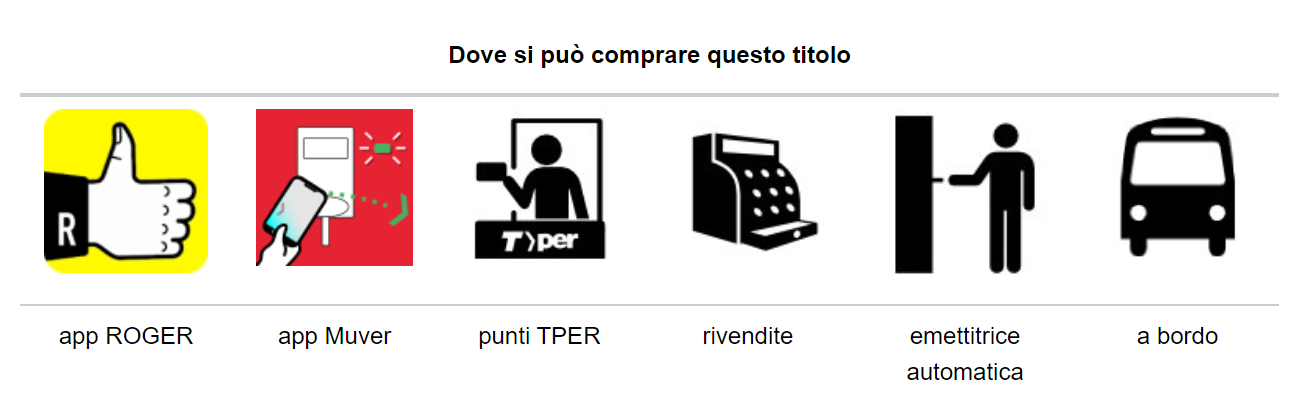
\includegraphics[scale=0.75]{biglietto}

\item  \textbf{十次票 City pass - 10 viaggi}\\
有效期为 10 次,每次 75 分钟。它允许你在任何路线上在博洛尼亚市区循环,甚至使用多条线路。也可以多人同时使用,每个人都需要打票,一次最多可容纳 7 名乘客。在多人同时使用一张多程票的情况下,必须在三分钟内同时打票,3 分钟后无法再添加乘客。例如,三个人同时使用,需要在3分钟内,连续打票三次。(14欧元/张)
\item  \textbf{日票 Giornaliero}\\
自打票之日起24小时内有效,可用于在博洛尼亚市区内任意路线循环使用,甚至使用多条线路。 它必须在第一次乘车时打票开始计算时间。(6欧元/张)
每次换乘时也需要重新打票。

\item  \textbf{年票 Annuale}\\
有效期为一年(从有效期开始算起365天),让你可以每天循环使用,不受行程和时间限制。年票是印有“Mi Muovo”的黄色卡片,其工本费为5欧元,有效期为5年,在Tper销售点出售。如果遗失,补办费用也是5欧元/张。该卡实名制,所以不支持转让使用,每次上车都需要打票。(年票标准价格300欧元/年,另有优惠价格:27岁以下的青年为220欧元/年,70岁以上的老人190欧元/年。博大在读学生通过学生主页Studentionline购买的优惠价格为180欧元/年,来博大的交换生则可以用象征性的10欧元购买一张可以在交换期间使用的公交车卡)。
\item  \textbf{月票 Mensile}\\
36欧元/月。27岁以下的青年,优惠价格为27欧元/月。每次上车都需要打票。可以在网上购买或者去Tper窗口购买。其有效期为首次打票的日期至当月月底。由于是非记名票,所以可以转让使用,但是不支持多人同时使用(例如不可以两人上车刷两次月票)。
\item  \textbf{使用非接触式卡支付}\\
目前在博洛尼亚、费拉拉和伊莫拉地区的公交车已支持使用非接触式卡在上车时购买车票,票价为1.5欧。使用方法为:上车后在如右图所示的绿色机器上刷卡即可。仅支持非接触式卡,即带有 
\includegraphics[scale=0.6]{carta} 标的预付卡、借记卡和信用卡。如果需要换乘,在换乘时请刷同一张卡,系统将会自动判定。\\
\textbf{注意!}\\
1、绑定在例如Apple Pay和Samsung Pay等支付软件中的卡和其对应的实体卡将被视为两张不同的卡!\\
2、在遇到查票员时,提供卡号的末尾四位即可。如果是绑定在支付软件中的卡,请提供其设备卡号而非实体卡号的末尾四位。\\
3、使用该方法乘车时,请在上车前通过车辆侧面的标识确认车辆有该刷卡机。首次刷卡购票后,如果你要换乘的车没有该机器或机器故障,则无需再次刷卡,且在75分钟有效期内没有受到处罚的风险。
\item  \textbf{费拉拉(Ferrara)和伊莫拉(Imola)地区的车票价格}\\
\textbf{费拉拉:}次票1.3欧元/张,日票3.5欧元/张,10次票12欧元/张。月票28欧元/张(不可转让给其他人使用),月票32欧元/张(不记名式,可以转让给其他人使用)。年票卡本费5欧元,标准价256欧元/张,优惠价格27岁以下为210欧元/张,70岁以上180欧元/张。\\
\textbf{伊莫拉:}次票1.5欧元/张,10次票14欧元,月票28欧元/张,年票标准价格为256欧元/张,卡片工本费为5欧元/张,优惠价格为27岁以下220欧元/年,70岁以上190欧元/年。


\item  \textbf{机场交通}\\
1、从机场乘坐出租车前往市区\\
根据时间和到达地点的不同,乘车费用可能在15到 25欧元之间波动。\\
2、机场轻轨“马可尼特快”(Marconi Express)\\
在中央车站和机场之间往返,每天从5:40 到 24:00,一年 365 天。单程用时约七分半,单程票9.2欧元/人,往返票17欧元每人。中央车站的乘坐地点为位于Via de'Carracci的高铁站的中庭内。可以在乘车点购买车票、在官方软件Roger上购买车票,也可以扫描下方二维码在线购买。\\
\\

\includegraphics[scale=0.3]{marconiqrcode}
%%(https://www.marconiexpress.it/biglietti/dove-acquistare-i-biglietti/)


\end{itemize}


\subsubsection{罚款}
\begin{itemize}
\item  75欧,如果5天内交罚款
\item  100欧,标准罚款
\item  300欧,如果因迟迟不交而产生滞纳金后所能累计的最高罚款
\item  6欧,如果乘车没带订阅票(年票、月票),需在5天内持订阅票和身份证件前往Tper服务点缴纳罚款
\end{itemize}
如果你使用的是27欧的青年折扣月票,你还需要在被查票时出示身份证件以证明自己的年龄。\\
如果被罚款,可以向查票员立即支付罚款,或者拿上罚单到Tper窗口支付罚款。如果不当场交罚款,查票人会问你询问护照、居留、税号等个人信息,建议最好当场补交罚款,否则会记录个人诚信档案,对以后在意大利等欧盟国家办理信用卡、找工作造成一些不必要的麻烦。为了不遇到这种情况,大家最好上车打票,不要存在侥幸心理。\\
\\
\textbf{注意!}如果遇到打票机、购票机或非接触式刷卡机故障而造成的无法打票、购票,则可以报告给司机并在遇到查票员时说明情况。建议在遇到此情况时拍摄存留证据。\\
Tper服务点:扫描下方二维码查看\\
\\

\includegraphics[scale=0.3]{tperqrcode}
%%(https://www.tper.it/cliente/i-punti-tper)
\\
\\
\textbf{有关罢工}\\
罢工时,参与罢工的公共交通公司的官网、以及车站站牌上都会公布相关信息,上面能看到本次罢工影响的时间和区域。或者下载诸如“Moovit”等APP,即可收到实时提醒罢工信息和因集会游行而造成的线路改动的通知,也能查询的公交车时间表和实时位置。\\



\section{火车 (Treni)}

\subsection{意大利火车系统介绍}

意大利国铁(Trenitalia)官方网站: trenitalia.it 该网站可以查询火车时刻表、罢工信息、购买火车票等。\\
意大利的火车按速度和行驶范围一般可以分为多个档次:
\begin{itemize}
\item  \textbf{Regionale/Regionale Veloce} 普速列车,相当于国内火车的普快。两种类型的列车速度没有区别,但RV停的站会相对少些。其火车票灵活,类似公交票,乘坐车次和座位可以在上车后灵活选取,纸质票可在票上显示的当天晚上11:59之前使用。每小时的有效期从打票的那一刻开始。上车前必须在站台打票,未来得及打票的,上车后需要及时寻找列车员进行说明,他们会写上时间。\\
车程必须在打票后4小时内结束,特定区域费率规定的例外情况除外。\\
在线购买的车票在所选列车出发后4小时内有效,无需验证。\\
在车票有效期届满时上车的旅客可以继续已经开始的旅程到目的地车站,而无需中途停靠。
\item  \textbf{Intercity(IC) | Intercity Notte} 带有隔间的火车,站点相对少,相当于国内火车的快车。每个车票对应固定车次,固定座位。
\end{itemize}

意大利高铁系统发达,其速度根据线路的不同往往能达到300KM/小时。高铁列车分为:
\begin{itemize}
\item  \textbf{Freccia Bianca(白箭)、Freccia Argento(银箭)和Freccia Rossa(红箭)}三种,隶属意大利国铁。红箭速度最快,银箭次之,白箭相对最慢。车票对应固定车次,固定座位。银箭和红箭周六有2人行的折扣。
\item  \textbf{Italo} 私人高铁公司,性价比更高。车票对应固定车次,固定座位。
\end{itemize}

\subsection{购票方式}
\begin{itemize}
\item  \textbf{在线购买}\\
在Trenitalia,Italo官方网站购买:\\
https://www.trenitalia.com/\\
https://www.italotreno.it/it\\
官方软件:Trenitalia、Italo等;\\
第三方软件:Omio等;\\
高铁车票提前买折扣很大,如果你早就规划好了行程,建议提早买票。\\
\item  \textbf{线下购买}\\
火车站的自助售票机:\\
售票机一般分为两种,售卖Trenitlia车票的和售卖Italo车票的售票机,请注意区分。支持银行卡/现金支付车票。(机器语言可以选择中文/意大利语/法语/英语等);\\
\\
火车站里的人工柜台:\\
告诉工作人员出发和到达的地点,工作人员会让你选择时间。
但线下购买仅适用于城市市中心大车站,有些小镇的火车站经停站点并没有售票机和人工柜台,只能网上购买车票或者上车时立即向乘务员补票。
\end{itemize}
\textbf{注意:}\\
乘车:
博洛尼亚中央车站Stazione Centrale有很多站台(地上站台及地下站台,地上站台分为不同的方向,东、西广场等,地下则有很多层及停车场),如果是第一次乘车,请至少在发车前30分钟到达车站寻找乘车站台。在火车站乘车,请观看大厅的公告板 (Tabella luminosa) 的出发 (Partenza) 一栏,根据列车编号寻找乘车站台,不要被到达(Arrivi) 的时刻迷惑。在公告板上可以得知要坐的火车是哪个站台,是否晚点 (Ritardo) 。\\
\\
关于车票:
如果购买了Regionale和Regionale Veloce的纸质票,一定要在上车前打票。\\
\\
关于退改票:
高铁的火车票,具体是否可以更改或退款,取决于你购票时所享受的优惠,其退改信息(是否可以退改,退改的时间和手续费等)也会在购票页面写明,请注意查看。\\
\\
关于 Italo 特色车厢:
Italo高铁的Cinema车厢可以看意大利电影,但是需要自备耳机。如果想体验,请在购票时选择Cinema车厢。\\
\\
关于普速列车:如果所去地方仅是途经站,须看站台附近的打印版固定时刻表,黄色为出发,白色为到达。因为公告板 (Tabella luminosa) 主要显示的是起始站和终点站,途径车站滚动显示,不太方便查询。 \\
\\
此外,在Trenitalia官网上注册CartafrecciaYOUNG,如果是30岁以下通常可以享受青年优惠价,并且会时常有邮件推送折扣信息。另外还有学生优惠等,具体信息可查看官网。\\


\section{长途大巴 (Pullman)}
在意大利以及欧洲短途旅行或者长途旅行时,除了火车和飞机以外,还可以选择巴士出行。去同一个城市,坐巴士花的费用往往不到火车费用的一半。但是巴士班次较少,不像火车班次很多。如果是出国或者在意大利境内比较长途的旅行,还可以乘坐夜间巴士,通常是10个小时左右到达目的地,晚上出发,早上就到了,不耽误白天的时间。而且如果打折,有可能买到1欧的廉价票。缺点是在巴士上睡觉不是很舒服。
欧洲巴士系统十分正规且发达,有许多巴士公司供消费者选择,比较著名的有Flixbus、Eurolines、MarinoBus和Itabus等。巴士车票可以在其官网或第三方软件上购买,例如可以用支付宝付款的第三方车票预订软件Omio,综合了意大利很多公司的车票车次信息。
\subsection{购票方式}
以Flixbus为例
\begin{itemize}
\item  \textbf{网站购票:}前往Flixbus官网,选择路线和出发时间后,可以通过信用卡、Paypal、Google pay等多种渠道支付,付款成功后邮箱会收到确认邮件包括车次的具体信息。
\item  \textbf{App购票:}从App Store或Google Play下载FlixBus应用程序。预订车票后使用信用卡付款,付款成功后会收到确认邮件。
\item  \textbf{在销售点购票:}如果更喜欢购买实体车票,可以随时联系销售点预订巴士车票。 也可以前往隶属于Flixbus的旅行社,或前往意大利境内的众多售票处之一。\\
\textbf{以下是一些主要的Flixbus售票处:}\\
Ticketbus Central A - Bus Station, Largo Guido Mazzoni - 罗马\\
Milan Lampugnano Bus Terminal, Via Giulio Natta, 20151 米兰\\
Terminalbus 都灵,Corso Vittorio Emanuele Ii - 都灵\\
Vecchione Agency, Corso Arnaldo Lucci, 24 / Metropark - 那不勒斯\\
ATS S.R.L., Via Giuseppe Capruzzi 224 / C-226 - 巴里\\
Ticketbus Bologna Bus station, Piazza Xx Settembre, 6 - 博洛尼亚\\
Autostazione Trieste,Piazza Liberta '9 – 的里雅斯特\\
\end{itemize}
\textbf{有关其他巴士公司的购票请参阅其官网。}\\
\subsection{乘车地点}
博洛尼亚的乘车地点通常为Autostazione(Piazza XX Settembre 6),但是还请仔细检查购票网站/软件或车票上的说明。

\section{出租车 (Taxi)}
博洛尼亚的出租车主要由C.A.T.联盟运营,24/7全时段提供出租车服务。叫车方式有:\\
致电预约:051 4590\\
短信叫车:发送短信给333 333 0749或336 673 0000,写明乘车地址(街道名称,门牌号),随后会受到系统的回复。\\
使用APP:ItTaxi\\
车费:具体费用表请扫描下方二维码查看。\\
\\

\includegraphics[scale=0.3]{taxiqrcode}\\
%%(https://taxibologna.it/wp-content/uploads/2019/03/TARIFFARIO-ITALIANO.pdf)
\\
付款方式:支持现金、刷卡支付,如果使用ItTaxi叫车,也可以在App上支付。部分出租车也支持支付宝支付,付款码通常在副驾驶座位头枕后,详询出租车司机。


\section{私人租车 (Noleggio auto)}
驾龄超过一年之后才有租车的资格。租车可以在网上申请,然后到租车办事处领车。根据车型和淡旺季,租金40-100多欧/天不等。\\
欧洲流行的租车公司网站有(费用由低到高):
\begin{itemize}
\item https://www.europcar.it
\item http://www.avisautonoleggio.it/default.aspx 
\item https://www.hertz.it/rentacar/reservation/
\end{itemize}


\section{航空 (Aerei)}

\subsection{廉价航空}
在欧洲旅行首推乘坐各家廉价航空公司的航班,如果购票及时很有可能买到超级便宜的机票,而且航线广,欧洲各大城市都有涉及。以下为几家常用链接航空网站:
\begin{itemize}
\item www.ryanair.com
\item www.easyjet.com
\item www.vueling.com
\item www.opodo.it
\end{itemize}

\subsection{关于回国}
打算回国时可能遇到的情况:
\begin{itemize}
\item 第一种情况:第一次申请居留,手里只有居留条,不可以回国,除非签证在有效期内。
\item 第二种情况:持有过期居留,同时有居留条。可以乘坐直飞,不能在欧盟内其他国家转机,可以在俄罗斯、迪拜等转机。
\item 第三种情况:持有有效居留卡,怎么飞都是允许的,包括在申根国,俄罗斯、迪拜、土耳其转机。
\end{itemize}

\section{邮政|通信|网络}

\subsection{邮局常用到的几个业务}
\begin{itemize}
\item 邮政储蓄。可以办理银行卡,和其他银行服务相同。
\item 邮寄业务。挂号信(Raccomandata)是法律性质强的邮寄方法。尤其办理奖学金材料时用到。邮寄前先在窗口领取表格填写,避免延误时间。领取时可以不排队。
\item 居留申请。邮寄居留表格之前,不要忘记购买16欧的印花税。
\item 其他杂务: 水电煤气费用、保险、医药费用等,每张缴费单子(Bolletta)需多缴纳1.3欧的手续费(Commissione),如果在烟草店(Tabacchi)缴费,需多缴纳2欧的手续费。

\end{itemize}

\subsection{快递}
意大利境内主要快递公司包括:DHL、TNT、UPS、FedEx、PosteItaliane 等等。
\begin{itemize}
\item DHL:服务好,送货速度快,但价格更贵。从国内邮寄文件,小物品比较合适,一般3-5个工作日。
\item TNT:意大利最常用的快递公司,价格更便宜,国内EMS包裹到意大利一般也由TNT接管。
\item FedEx: 美国联邦快递,是快递中寄往中国海关税收得最低的公司。
\item PosteItaliane: 意大利邮政,优点是便宜,缺点是时间太慢,不论是在意大利境内的投递还是邮寄回中国都很慢,少则一个月,多则三个月不等。并且在寄回国以后还需要缴纳一定程度的海关税。
\item 人肉快递:目前价格约30欧/公斤靠上,国内邮寄费用另算。可在学联QQ群、本地微信群内寻找。
\end{itemize}

\subsection{通信}
意大利的国际电话区号是 0039 (+39)。意大利各地区区号都以 0 开头,如米兰 02、罗马 06、博洛尼亚 051 等。所以从中国拨打意大利博洛尼亚市的固定电话的方式为:0039+051+固定电话号码。意大利手机使用的手机网络模式与中国一致,均为 GSM 模式,所以大部分的中国手机在意大利均可以直接使用。意大利主要的手机运营商有四个,分别是 Wind、Tim以及Vodafone。 \\
办理手机卡的方式为:选择一个运营商,前往其线下店,告诉工作人员要办理新的电话卡,选择你喜欢的套餐,出示护照和税号即可。\\
\\
意大利所有运营商均支持携号转网。选择你想转到的运营商,前往其线下店,告诉工作人员你想转到新的运营商,选择你喜欢的套餐,出示护照和税号即可。工作人员会给你一张新的卡,当你的旧卡无法使用时,新卡就可以使用了,一般在两天左右。\\



手机充值方式一般有三种:
\begin{itemize}
\item 去烟草店(Tabacchi)充值。 
\item 去自己运营商的官方网站充值,可以使用信用卡、Paypal等。 
\item 下载自己运营商的APP,用APP充值,同时也能查看自己的流量剩余,套餐使用情况。
\end{itemize}
打电话回国,中国的国际电话区号为0086,因此从意大利打往中国的电话的拨号方式为:国内固定电话:0086+国内区号(去掉前面的0)+固定电话号码。例如打到天津:0086+22+固定电话号码。国内手机:0086+国内手机号码(不需要在手机号码前加0)。

其他注意事项:意大利全境无漫游费,所以在佩鲁贾或者锡耶纳办理的电话卡在意大利的其他城市也是一样的资费。 
\subsection{网络}

\begin{itemize}
\item 宽带上网:意大利主要网络运营商包括Fastweb、Tim、Infostrada(Wind 公司品牌)及Vodafone等。办理需要带着证件、税号、银行账号、家庭住址等。
\item 户外上网:麦当劳,政府的市政厅或者大学,机场往往都提供免费网络。
\end{itemize}
 
\chapter{生活信息}              

\section{夏令时} 

从每年3月的最后一个星期天到当年10月的最后一个星期天,意大利全国都要实行夏令时,以充分利用日光、节约能源。变更方法:三月最后的一个星期天早上2:00变更为3:00,夏令时开始,和中国时差为6个小时;10月的最后一个星期天早上3:00变更为2:00,夏令时结束,和中国时差为7个小时。

\section{安全问题}

\subsection{常用的紧急电话}

\begin{itemize}
\item 宪兵 (Carabinieri) : 112 
\item 国家警察(Polizia di Stato): 113 
\item 儿童救助(Emergenza Minori): 114
\item 消防警察(Vigili del Fuoco): 115 
\item 交通事故(Pronto Intervento):116 
\item 经济纠纷(Guardia di finanza): 117
\item 急救车(Pronto soccorso): 118
\end{itemize}

\subsection{安全与求助}
上街时要小心,特别是人多的地方及上下车的时候,避免给小偷下手的机会。出行一定要遵守交通规则。晚上单独出门时,如果遇到突发情况,及时请求宪兵或警察,千万不要客气。然后再根据事情严重程度,联系学联或中国驻意大利使领馆等。

\subsection{失物招领}
如果被盗或被抢劫请先去警察局报案(Denunciare),开立报案证明。之后补办证件、卡片、前往失物招领中心领取物品等均需用到报案证明。各地政府均设有失物招领中心,详情请参阅本地市政府官网。
\\
建议:易遗失的个人物品(手机、钱包等)里放上写有个人联系方式(例如手机号、邮箱等)的纸条,如果有人拾得并交给失物招领办公室,会联系你取回。

\subsection{Bologna 市失物招领中心}
\textbf{Comune di Bologna - Ufficio Oggetti Smarriti}\\
地址:Piazza Liber Paradisus, 8,B座0层\\
邮箱:ufficiooggettirinvenuti@comune.bologna.it\\
电话:051 2197070 \\
办公时间:\\
周一、周三和周五:8:00-12:30\\
周二:8:30-12:30 14:30-16:30\\
周四:8:30-16:30\\
访问失物招领办公室需要通过邮件预约。\\



\section{驾照}

中国驾照在双认证之后于欧盟境内有效期一年,所以有条件的同学尽量考取意大利驾照,该驾照10年一续,而且在欧盟范围内都有效。\\
意大利考驾照包括2个考试,一个道路法规理论考试(意大利语),一个是路考。理论考试共40道题,错题不能超过4个,题库约7000道。路考为人工考试,往往在郊区道路上考。博洛尼亚地区考驾照最快2个月能拿到,预算为1000多欧元。其中一多半钱数为练车费用。\\
考驾照需要准备的材料为:
\begin{itemize}
\item 意大利身份证 (Carta d'identità)
\item 税号
\item 3张照片
\item 健康证明(Certificato Medico Amnestico),健康证明由私人医生开具,证明费用30-50欧。
\item 居留
\end{itemize}
材料准备全,或快全了之后可以到离自己最近的驾校注册。注册费用350-650欧,根据是否有促销活动。理论考试过后会得到练车许可(Foglio Rosa),有资格预约练车。练车费用博洛尼亚的地区为38欧/小时,购买练车套餐(pacchetto)会有优惠。路考过后驾照当场发。无论理论还是路考,如果试失败,则须至少等1个月才能再考。理论补考费为150欧,路考补考费200欧。理论最多考3次,路考最多考2次,如果超过指定次数,则须重新注册驾校,重新开具所有证明。

查询附近的驾校,可以在谷歌地图上搜索Autoscuola。





 
\chapter{生活与购物}              



\section{中国超市}



\begin{itemize}
\item 兴隆超市, Market Alimenti Asiatici\\
地址: Via Corticella 26/C, 电话: 3208036711, 3273422087\\
商店经营: 鲜肉,蔬菜,冰冻海鲜,火锅料,生活用品,温州特产

\item 新中国-食品店,Alimenti Orientali e Macelleria\\
地址: Via Pietro Faccini 2-4(Via Ferrarese附近), 051-5874110, 3479111999\\
微信: chinatrade-bo\\
商店经营: 肉类,海鲜,蔬菜,佐料,滋补品,名酒,南北杂货等等\\
特色服务: 可以电话预订,送货上门。
\end{itemize}



\section{中餐厅}
\begin{itemize}
\item 茉莉花, Ristorante Jasmine\\
地址: Via Augusto Righi 3/B, 电话: 051-264908/3319199608 \\
营业时间: 周一关门\\
特色服务: 火锅

\item 如意, Ristorante RUYI\\
地址: Piazza Otto Agosto 30/A, 电话: 051-245615\\
菜类: 中餐,日餐。\\
网址: ristoranteruyi.it \\
营业时间: 11:00-15:00/18:00-23:30\\
特色服务: 包餐
\end{itemize}


\section{意大利超市}
\noindent 博洛尼亚主要超市有:Pam, Coop, Conad, Carrefour\\
巨型超市:IperCoop,Esselunga,Eurospar\\
廉价超市: Lidl, Ins, Penny, Eurospin\\
小型超市:Metà,inCoop,Pam local\\
蔬菜超市: Verdurra\\
超市位置,营业时间和到达方式均可在谷歌地图上查到。

\section{西餐厅}

\subsection{味美价廉}
人均20欧左右,或以内的。

\begin{itemize}
\item Osteria dell'Orsa\\
地址: Via Mentana, 1\\
菜类: 博洛尼亚地区菜,头道菜往往才7欧左右。

\item La Bella Napoli\\
地址: Via S. Felice, 40\\
菜类: 正宗那不勒斯披萨饼,那不勒斯地方菜

\item Nicola's Pizzeria Ristorante\\
地址: Piazza S. Martino, 9\\
菜类: 大号,丰盛的披萨饼

\item To Steki\\
地址: Largo Respighi, 4E\\
菜类: 希腊菜,丰盛的希腊烤肉10欧左右便能吃到,20欧左右吃到撑。

\item Delogo\\
地址: Via Giovanna Zaccherini Alvisi, 19\\
菜类: 希腊菜

\end{itemize}

\subsection{高档餐厅}
人均30-40欧,米其林80-100欧左右。

\begin{itemize}
\item Trattoria Gianni\\
地址: Via Clavature, 18\\
菜类: 博洛尼亚地区菜

\item Ristorante Diana\\
地址: Via dell'Indipendenza, 24\\
菜类: 博洛尼亚地区菜

\item Ristorante Pappagallo\\
地址: Piazza della Mercanzia, 3\\
菜类: 博洛尼亚地区菜, 高档餐厅装潢

\item Cantina Bentivoglio\\
地址: Via Mascarella, 4/b\\
特色: 意大利北部菜,酒窖,jazz音乐会

\item I Portici Hotel\\
地址: Via dell'Indipendenza, 69\\
菜类: 米其林星级餐厅

\item Aroma de Roma\\
地址: Via Alessandrini, 19/D\\
菜类: 罗马菜
\end{itemize}


\section{衣物}
\begin{itemize}
\item PRINCESS Calzature皮鞋店\\
地址: Via dell'indipendenza 44F, 52A, 电话: 051-247937\\
经营品牌: Armani, Armani Jeans, MK, CK, Sendra, Moschino, Pollini, Hugo Boss, Cesare P., John Richmond, Waller\\
皮鞋纯意大利手工制作
\end{itemize}

\section{意大利主要打折村}
\begin{multicols}{2}

\subsubsection{THE MALL(佛罗伦萨附近)}
\noindent 网址:www.themall.it\\
主要品牌:Gucci, Prada, Armani, Bottega Veneta, Coach, Dior, Burberry, Tod’s, Valentino, Ferragamo, Balenciaga, Zegna, Fendi, Roberto Cavalli, Sergio Rossi ...\\
地址:Via Europa 8,50060 Leccio Reggello,Firenze(离佛罗伦萨30km)。\\
营业时间:周一至周日10:00 - 19:00 \\
前往: Autostazione Sita Firenze 乘themall专车, 单程10欧,30分钟到达。

\subsubsection{Barberino Designer Outlet佛罗伦萨附近)}
\noindent 网址: www.mcarthurglen.com/barberino-designer-outlet\\
主要品牌:Ralph Lauren, Prada, DolceGabbana, BOSS, Cavalli, Nike, Adidas 等等\\
地址:Via Meucci snc, 50031 Barberino di Mugello (FI)\\
前往:Piazza della Stazione n.44 乘专车,往返15欧,30分钟到达。
 
\subsubsection{SERRAVALLE DESIGNER OUTLET(米兰附近)}
\noindent 网址:www.mcarthurglen.it/serravalle\\
主要品牌:PRADA,VERSACE,FERRAGAMO 等170多家。\\
地址:Via della moda,1,15069 Serravalle Scrivia(AL)\\
前往:Foro Bonaparte 乘专车, 往返20欧,
 
\subsubsection{Veneto Designer Outlet(威尼斯附近)}
\noindent 网址:www.mcarthurglen.it/noventadipiave \\
主要品牌:Bottega Veneta,Prada,Ferragamo,Fendi,Versace, Armani,Burberry ... \\
地址:Via Marco Polo1,30020 Noventa di Piave(VE) \\
营业时间:周一至周日10:00~20:00\\
前往:Venezia Tronchetto 乘专车,往返15欧。
 
\subsubsection{Fidenza Village(帕尔马附近)}
\noindent 网址:www.fidenzavillage.com\\
主要品牌:Versace,Guess,CK,Levis,Pinko,Samsonite等100家店\\
地址:Via San Michele Campagna,43036 Fidenza PR\\
前往:摆渡车从Stazione Fidenza发车,车票0.50欧,车上购买。

\subsubsection{Castel Guelfo, The style outlets(博洛尼亚附近)}
\noindent 网址:castel-guelfo.thestyleoutlets.it\\
主要品牌:CK Jeans, Levis, Liu.Jo, Nike, Samsonite, Desigual, Adidas, Nike 等等\\
地址:Via del Commercio, 4, 40023 Castel Guelfo di Bologna\\
前往:摆渡车从Stazione ferroviara di Castel S. Pietro Terme免费到达打折村,5min路程

\end{multicols}
\chapter{博洛尼亚景点}              


\section{博洛尼亚景点}

\subsubsection{Due Torri 双塔}
双塔是博洛尼亚的两座斜塔,博洛尼亚诸塔中最著名的两座,也是该市的标志。它们位于通往五个城门的道路的交叉口。较高的一座名为阿西内利塔 Asinelli,高97.2米;较低加里森达塔 Garisenda 更为倾斜,高48米, 它们得名于建塔的家族,建于1109年到1119年。其中Asinelli可攀登游览。\\
开放时间:分为三季度,时间待定。 门票:3欧


\subsubsection{Piazza Maggiore 主广场}
主广场是博洛尼亚的心脏,这里见证了博洛尼亚历史的变化。在很久以前,这里是一片草地,从1200年开始,当地政府开始收购土地,建立房屋,尤其是今天环绕广场的政府办公大楼。而在广场中央,当时的人们搞各类商品的买卖活动。之前这里称作Curia Communis,之后叫Platea Communis, 大约从1500开始,这里改名为Piazza Maggiore,之后改为和意大利国王Vittorio Emanuele II同名,然后在1945由改回了Piazza Maggiore的名字.
 
\subsubsection{Palazzo dell'Archiginnasio 大学旧址}
大楼建于1562和1563之间,由工程师Antonio Morandi主管,建设目的主要为了当时研究法学和艺术学的大学所建立. 一直到1803年,这里一直是大学的主楼,从那以后,这边变成了民族图书馆。在1944年,大楼严重的被二战时期的炸弹损坏,之后有修复。大楼里面依然保存几个重要的房间,比如,如今的Sala di lettura是当时的艺术学教室,如今的Sala dello Stabat Mater是当时的法学教室。大楼内部的墙上的勋章一部分是纪念名师的,一部分是学生家族的徽章。入口对面的建筑里面有着著名的解刨室,又名S.Maria dei Bulgrai礼拜堂。这个屋子由Antonio Levante在1637年专门为解刨学修建。在这个屋子里,有一个著名的剥皮人Ercole Lelli的雕像。值得注意的是,据说人类最早的整形手术正是起源于博洛尼亚,因为当时有割五官的酷刑,医生为了尽全力医治受伤的人,开启了西方整形学的研究。


\subsubsection{Cattedrale Metropolitana di San Pietro 主教堂}
天主教博洛尼亚总教区的主教座堂。位于Via dell'Indipendenza,7 ,教堂始建于1028年,1141年毁于大火,1184年教宗下令重建。根据Gabriele Paleotti枢机主教的命令,1575年再次重建。1582年升格为“Cattedrale Metropolitana”。1743年到1747年最后一次重建。内部完全为巴洛克式,显得宏伟壮观。\\
开放时间:7:00-19:00\\
门票:免费

\subsubsection{Basilica di San Petronio 大教堂}
博洛尼亚的主要教堂,但并非该市的主教座堂。是世界上最大的砖砌哥特式教堂,长132米,宽60米,顶高45米,立面高51米,可以容纳28000人。San Petronio是5世纪的博洛尼亚主教。该教堂始建于1390年6月7日,工程持续了几个世纪,完成于1663年。\\
教堂拥有两座管风琴,其中一座为目前世界上仍然可以演奏的最老管风琴。教堂内还有世界上最长的日晷\\
开放时间:8:30-13:00 15:00-18:00\\
门票:免费

\subsubsection{Palazzo d'Accursio}
在2008年11月11日之前,为该市的市政厅。现为艺术博物馆,展出中世纪到19世纪绘画。宫内还设有莫兰迪博物馆,展出乔治·莫兰迪作品。内包含SALA ROSSA位于一楼,Galleria Vidoniana,建于1665年;Sala Falnese,Aula Piana,Sala Urbana位于二楼,顶楼是Collezioni Comunali d'Arte艺术馆。而Sala Borsa位于海神喷泉和Via Ugo Bassi交界的建筑内。Sala Borsa内含市政图书馆,可前往自习,以及办理借书证并借阅图书。\\
大厅和图书馆开放时间:周一:14:30-20:00;周二至周五:10:00-20:00;周六:10:00-19:00;周日和节假日关闭。\\

\subsubsection{Fontana di Nettuno}
海神喷泉,是博洛尼亚的一个巨大的喷泉,位于同名的海神广场(Piazza Nettuno),毗邻主广场Piazza Maggiore,海神尼普顿Nettuno的青铜雕像,伸出手臂,摆出傲慢的姿态,象征控制水域,是Jean de Boulogne较早的成熟作品,大约完成于1567年。

\subsubsection{Santuario Madonna di San Luca}
博洛尼亚的一座罗马天主教次级圣殿,位于老城西南方300米高的瓜尔迪亚山顶。
虽然现在有一条公路通往这个朝圣地,但是仍可以通过一条长达3.5公里的带屋顶的有666个拱的圣路加拱廊(Portico di San Luca)前往,圣路加拱廊建于1674-1793年,是为了在游行上山时保护圣像。每年的游行要从圣彼得在博洛尼亚市中心的圣伯多禄主教座堂,沿着这条路线前往朝圣地。


这个朝圣地收藏了一幅圣母像。山顶的教堂已经存在了一千年左右。目前这座教堂建于1723年,使用了Carlo Francesco Dotti的设计。堂内收藏有不少艺术品。\\
地址:Via di San Luca, 36,乘坐20路公交车可以直达山脚下。\\
开放时间:7:00-18:00\\
门票:免费

\subsubsection{Portici di Bologna}
博洛尼亚市内处处可见拱廊,它们的落成时间为12世纪至今,总计约62公里。这些拱廊有的以木材建造,有的以砖石砌就,还有的以钢筋混凝土浇筑,俯瞰着街道一侧或双侧的道路、广场、小径或人行道。拱廊常以带顶人行道和黄金商业区的形式出现,因而广受欢迎。这些拱廊代表着不同的类型、城市和社会功能以及时间阶段。拱廊被视为服务公众的私有财产,已成为博洛尼亚城市身份的一种要素和表现形式。2021年,城内最具代表性的12处拱廊及其周围建筑被选入世界遗产名录。

\subsubsection{Marzabotto}
据考古遗址发现,远在旧石器时代,意大利半到已经出现人类活动的遗迹,他们使用石制物品,工具。新石器时代,他们已过着畜牧和渔猎生活。公元前两千多年,印欧语系民族在波河平原定居,公元前8世纪,埃特鲁里亚人取代维拉诺维安人成为破河流域的主人,意大利的历史也因而进入伊特拉士坎时期。埃特鲁里亚人大多身材壮硕,个子不高,浓眉、鼻弯;女性则美艳。善于手工制作器具,发展出灌溉和排水设施,在建筑技术上,善于开采矿石,在住屋周围建巨石,商业贸易繁荣,制陶业兴盛;宗教信仰方面特别重视“神的旨意”;另外他们作战能力较强,军事技术优越。因此,公元前6世纪在国王及贵族引导下迅速扩大势力,达到鼎盛时期。范围囊括整个波河流域,并占据中部拉丁姆平原。随后因内部分裂逐渐衰落,加之在与罗马人战争中战败,城邦被吞并,失去统治地位。公元前3世纪和罗马人融合,也被同化。作为意大利古民族之一,其文化仍影响至今,且现存多处遗址古迹供游人参观。其中最具代表性的一处当属Marzabotto, 位于博洛尼亚以南仅几十公里的山间小镇,人口稀少但却依山傍水,更有多处埃特鲁里亚人古城邦遗址及一座博物馆,对于喜好古代人文的同学来说是一个不错的周末散心首选之地。

到达方式:从博洛尼亚中心火车站乘坐火车到Marzabotto站下车,出了火车站一路向西走到快速路Via Porrettana,再沿路向南走一点即到。遗址区域名为:Museo Nazionale Etrusco e Area Archeologica.
\\
\\
\\
\\

\section{推荐博物馆}

\subsubsection{Pinacoteca Nazionale Bologna 国立博洛尼亚美术馆}
主要展示 13 至 18 世纪艾米利亚地区画家的作品,另外还有少数博洛尼亚世界著名画家莫兰迪的几幅素描。\\
地址:Via delle Belle Arti 56, \\
门票:全票6欧,博洛尼亚大学建筑学、文化遗产、人文学与哲学学生以及美院学生免费,18-25岁可享受折扣2欧票价。\\
开放时间:周二、周三:9:00-14:00;周四至周日:10:00-19:00\\
官方网址:https://www.pinacotecabologna.beniculturali.it/it/

\subsubsection{MAMBO}
Museo d'Arte Moderna di Bologna 博洛尼亚现代艺术博物馆,是意大利最主要的现代和当代艺术博物馆之一,是一个博洛尼亚的艺术组织所在地,主要研究当代艺术。现有展品既有永久保存在博物馆的,,也有暂时展出的藏品。 并且长期展出博洛尼亚世界著名艺术家莫兰迪的展品。\\ 
MAMBO内有一所图书馆、一间书店和一个酒吧餐馆(Bar/Ristorante)。\\
开放时间:周二、三:14:00-19:00;周四:14:00-20:00;周五至周日:10:00-19:00。\\
票价:全票6欧;减免票价4欧;18-25岁年轻人2欧;大学学生持学生证免费参观;对于永久展出藏品,每个月的第一个星期日免费参观。\\
官方网址:http://www.mambo-bologna.org/

\subsubsection{Museo Civico Bargellini  工艺美术馆}
美术馆是一座建于十七世纪的宫殿,由建筑家Bartolomeo Provaglia 设计,这座宫殿是抛弃以往的传统拱门式结构风格,来凸显其独特和庄重;与圣母忠仆圣殿相邻,圣母忠仆大殿(Basilica di Santa Maria dei Servi)是博洛尼亚的一座天主教宗座圣殿。这座教堂长100米,宽20米,创建于1346年,是属于圣母忠仆会的教堂。庇护十二世将其升格为宗座圣殿。从外面看,这座教堂非常简朴,立面分为几段,没有装饰。值得注意的是它的建于16世纪的庭院,模仿了伯鲁乃列斯基在佛罗伦萨所建孤儿院的拱廊。教堂前面的广场很小,在周围兴建了环绕整个广场的拱廊。拱廊的一侧是修女院,另外两面向街道开放。该市有为数不少的拱廊街,其中一些源自古罗马时代。
在圣母忠仆圣殿前还留有拱廊开放式空间,入口处有两个由Francesco Agnesini 和Gabriele Brunelli 雕塑制作的男性雕塑柱。博物馆包括贵族和资产阶级,工具,饰品,陶瓷,绘画等收藏物。\\
地址:Strada Maggiore, 44\\
开放时间:周二至周四10:00-15:00;周五14:00-18:00;周六和周日10:00-18:30。\\
\chapter{UNIBO - 博洛尼亚大学}    

\section{大学简介}
Alma Mater Studiorum - Università di Bologna,博洛尼亚大学,创立于公元1088年神圣罗马帝国时期,是世界上广泛公认的、拥有完整大学体系并发展的第一所大学,被誉为“世界大学之母”。在以拉丁语为主要学术与研究通用语言的中世纪及近代欧洲,博洛尼亚大学始终保持着欧洲文化与学术发展的中心位置,并引领了欧洲大学体系的改革。官方拉丁文校名直译为“大学之母”(Alma Mater Studiorum)。1988年在430所欧洲大学校长共同签署的“欧洲大学宪章”中,博洛尼亚大学被正式宣称为欧洲所有大学的母校。

在大学900多年的历史里,涌现了众多杰出校友,包括文艺复兴时代的开拓人物但丁、提出太阳中心说的天文学家哥白尼,以及彼特拉克、丢勒、伊拉斯谟、哥尔多尼、马可尼、安伯托·艾柯、罗马诺·普罗迪、皮埃尔·保罗·帕索里尼等著名人物都曾在这里学习或执教。
 
博洛尼亚大学是全球大学高研院联盟(UBIAS)、欧洲研究型大学联盟(LERU)、同一个欧洲大学联盟(Una Europa)、国际公立大学论坛(IFPU)、科英布拉集团(Coimbra Group)、欧洲大学联盟(Europaeum)、乌得勒支网络(Utrecht Network)、中国-欧盟IRES-8合作等著名高校组织的核心成员。

博洛尼亚大学位列2023U.S.News世界大学排名第122位,2023泰晤士高等教育世界大学影响力排名第23位,2024QS毕业生就业竞争力排名第97位。

作为经历了近千年历史演变的教育机构,博洛尼亚大学的校园建筑保留了不同时期,特别是文艺复兴时期的众多特点。博洛尼亚大学曾被福布斯杂志评为全球最美的15所校园之一,2014年被世界最大的英文旅游信息出版商福多尔公司评为全球15所最值得访问的大学之一。博洛尼亚大学校园建筑面积117万平方米,总面积674万平方米,除了位于博洛尼亚的主校区之外,大学还有四个分校区,分别位于切塞纳、弗利、拉文纳和里米尼,另外在布宜诺斯艾利斯设有海外校区,在布鲁塞尔、纽约和上海设有办事处。

\section{招生公告}        

大学各学院在年末会公布来年招生公告(Bando di Ammissione),公告会详细说明来年的招生计划、招生名额、注册及考试流程,对入学流程有任何困扰的同学,请仔细查阅该公告。\\
公告的下载途径为:访问您感兴趣的专业官网,点击“Iscriversi”、随后选择“Iscriversi al Corso: requisiti, tempi e modalità”、下载“Bando di Ammissione A.A. 202X/202X”

\subsection{Studenti online网站注册}
新生必须使用自己的税号(尚未拥有税号的可使用自己的个人身份信息)在大学内部系统Studenti online上注册,得到自己的用户名及密码。随后登录,并通过此系统注册入学、报名考试、打印各类证明及查看自己大学生涯等等。请注意各专业申请的截止日期。如果考试顺利,但是错过了申请截止日期,依然会被取消入学资格。\\
网站为https://studenti.unibo.it/sol/welcome.htm,你可以扫描下方二维码访问\\
\\

\includegraphics[scale=0.3]{studentionlineqrcode}\\
%% https://studenti.unibo.it/sol/welcome.htm

\subsection{马可波罗计划}
为中国学生提供的马可波罗计划,旨在欢迎并帮助中国学生入读意大利的大学。得益于本计划,对于想来意大利就读大学的中国学生,即使不懂意大利语也能获得入境签证。该计划要求学生在入读大学课程之前,在参与并遵守该计划的语言学校内学习10-11个月的意大利语课程。


您可以在佩鲁贾外国人大学、锡耶纳外国人大学、罗马第三大学、“Dante Alighieri”协会(即但丁语言学校)、雷焦卡拉布里亚外国人大学参加针对马可波罗计划生的意大利语课程。您还可以参加其他参与并遵守马可波罗计划的意大利大学的意大利语课程,部分私立语言学校也可以提供该课程。


\textbf{值得注意的是,}从2022/23学年起,马可波罗计划生将不再享有以往的专用名额,您需要与居住在其他非欧盟地区的学生平等竞争。\\

\subsubsection{计划生注意事项}
\begin{itemize}
\item 抵意后,必须在您预注册文件中指定的时间参加意大利语课程,不得参加非您预注册语言学校的意大利语课程。博洛尼亚大学不为马可波罗计划生提供语言培训课程 
\item 马可波罗计划生必须通过上述意大利语课程的考试,以至少达到由欧洲委员会承认的B1水平,并且获得以下意大利语证书之一:CELI B1(由佩鲁贾外国人大学颁发)、CILS B1(由锡耶纳外国人大学颁发)、PLIDA B1(由但丁语言学校颁发)和CERT.IT B1(由罗马第三大学颁发)。无论您选择的语言学校的课程进度安排如何,您都必须在2023年12月28日之前通过至少为B1水平的语言考试。
\item 如果语言学校拥有独立语言证书,则只能提供该校的语言证书。例如您在佩鲁贾外国人大学参加语言课程,则您只能提供由其颁发的CELI B1语言证书。如果语言学校没有独立语言证书,您可以提供以上四种中任意一个博洛尼亚大学认可的证书 
\item 您必须通过Studenti Online验证您的语言证书。访问Studenti Online,选择“Bandi”,随后选择“Programma Marco Polo per studenti cinesi a.a. 2023/24 - verifica certificati di lingua italiana”,上传您的语言证书和您的护照的PDF电子版。国际生办公室将对其进行审查,并在Studenti Online上发布结果。审查日期为2023年6月1日至2023年12月28日。如果因必要原因,您无法在此期间提供证书,请联系国际生办公室(internationaldesk@unibo.it)
\item 您需要在入学时,或无论如何都必须在2024年2月29日之前,将证书交付给您所就读专业的秘书处
\item 马可波罗计划生无需、也不得参加为非欧盟学生提供的CISIA意大利语测试
\item 您不能提交非上述所列的意大利语水平证明
\item 请记住,马可波罗计划生只能注册以意大利语授课的学习课程。
\end{itemize}


\subsection{入学要求}
所有专业分为:有名额限制(Numero programmato)和无名额限制(Libero accesso)两类。\\
\\
\textbf{有名额限制:}指该专业有录取名额限制,需要通过考试参与排名,按成绩高低进入录取名单(Graduatorie)后才能注册大学(Immatricolazione)。如过您的入学考试总分数或部分分数低于招生公告规定的分数线,则第一学年需要修OFA课程,在未完成OFA课程及考试前则无法进行第二学年课程的考试。\\
该类型的录取针对国际学生(居住在非欧盟地区)会有专用名额,详细信息请查看各专业的招生公告。\\
\\
\textbf{无名额限制:}指该专业无录取名额限制,无需参与排名,但招生公告中要求的考试必须参加。如果报名人数未超过意大利教育部规定的名额(取决于国际生人数名额和报名情况),则可以直接入学。如果入学考试总分数或部分分数低于招生公告规定的分数线,则第一学年需要修OFA课程,在未完成OFA课程及考试前则无法进行第二学年课程的考试。
\\
注意:部分专业的部分情况或许会有补录机会(Recupero),详情请看各专业的招生公告,补录需要自己申请!

\subsection{入学考试}

\subsubsection{本科和本硕连读(Laurea e LM a Ciclo Unico)}
分为:\\
1、需要参加TOLC考试的专业。\\
本科或本硕连读的专业都有可能要考TOLC考试,具体请通过查看自己专业的入学页面和招生公告来确定自己需要考的TOLC考试的类别。TOLC考试需要通过注册CISIA官网https://www.cisiaonline.it/,随后报名并参加考试。在通过考试后,需要参照专业的招生公告的要求参加排名(Selezione)。注意:中国学生只能参加给非欧盟学生(Studenti non UE residenti all'estero)的排名(一般为最后一次)。\\
\\
2、需要参加意大利教育部颁布的国家统一考试的专业。例如:Medicina Chirurgia、Medicina Veterinaria、Professioni di Architteto、Professioni Sanitarie etc等,阅读专业的招生公告,按步骤注册考试,在规定的日期参加考试。\\
\\
3、部分少量专业,其入学考试既不是TOLC考试也不是国家统一考试,其考试类型和方式请细读该专业的招生公告,按照其流程进行考试和入学。

\subsubsection{硕士(Laurea Magistrale)}
入学申请一般分为两个步骤:\\
1、本科背景审核部分(Requisiti Curriculari)\\ 
根据申请人的海外本科毕业范畴,审核依据本科期间的考试成绩和本科修的课程类别。\\
\\
2、个人准备部分(Valutazione delle Cometenza Personali)\\
每一个专业有不同的步骤。可能是一封动机信,可能是个人档案评估、面试、英语要求或一个测试。有关信息,请咨询您的专业的教授。


\subsection{正式注册入学}
在完成了入学前的步骤(获得语言证书、参加入学考试并被录取)后,需要在招生公告要求的截止时间内,进行网上注册并支付第一部分的注册费(157,04欧)。之后,可以通过Studenti online预约博洛尼亚大学相关学生秘书处(主校区为国际生秘书处,分校区则为各自校区的学生秘书处)提交材料,进行原件审核并完成注册。
注意:只有当你获得打印学生证的二维码后才算完成大学注册。
\\

所需材料:
\begin{itemize}
\item 填写好并签名的入学申请表格 
\item 缴纳第一期注册费的收据
\item 意大利语水平证书(英文授课专业请提交相应语言证书)
\item 经翻译双认证的高中毕业证书或毕业证和学位证(从大学毕业时取回)
\item 个人证件照
\item 居留或申请居留的回执
\item 护照复印件
\end{itemize}


\section{入学之后}
大学网站系统发达,各类信息应有尽有。网址:https://www.unibo.it/it 。关于个人信息,可以登录到Studenti online进行管理,通过考试系统(AlmaEsami)预约考试、交学费、开注册考试证明(Autocertificazione)、选取选修课等
如果想要快速找到自己专业的网站,可以通过谷歌搜索,输入“专业名称 Unibo”即可。在自己专业的网站上能查到详细的课程表(Orari di lezioni),学习计划(Piano di studio),在学习计划里面能找到细致的课程描述,参考书,考试方式介绍等等。

\subsection{ALMAWIFI}
ALMAWIFI 是博洛尼亚大学提供的无线网,覆盖所有校区和学生宿舍,注册生都可以登录。具体登录方法请查看后文 7.5.6 有关章节。

\subsection{次年注册手续}
入学一年以后,直至取得新的学位之前,学生都必须无条件的按年缴付学校规定的注册费。注册费缴付之后,即成功注册了新一学年的学习。除此之外,外国学生还需要注意,旧的居留证过期后,应随时向秘书处递交更新之后的居留证复印件,或者新的居留证申请回执复印件。因为若缺少有效的居留证件,新一年的注册将不会被系统识别,这将会影响到日后考试的注册以及分数登记(Verbalizzazione)。 居留条的递交能保持你的学籍6个月有效。

\subsection{学费}
学费,也即注册费,可以登录Studenti online后查看。通过上面的支付码可在意大利境内任何一家UniCredit银行缴纳学费。同时,也可使用信用卡通过pagoPA系统进行网上缴纳。每期费用均需在截止日期前缴纳完毕,若逾期未缴,将处以30欧(30天内),150欧(多于30天)的罚款。 

大学并不会对应缴金额和缴费截止日期做出任何主动告知行为,您需要自行查询相关金额并主动缴纳。

有关2022/2023学年的学费金额,可以扫描下方二维码查看。该表对应为最高金额,并不适用于有费用减免的情况。\\

\includegraphics[scale=0.5]{2023tasseqrcode}\\
%%https://www.unibo.it/it/allegati/tasse/ImportiMassimiTasseUnibo2023_24.pdf/@@download/file/ImportiMassimiTasseUnibo2023_24.pdf

根据大学的最新政策,2023/2024学年,作为国际学生,您的学费将根据您的原籍国和您的家庭有收入和资产的国家/地区计算。中国作为非经合组织国家,在享受该政策的国家名单中。该学费减免政策可于注册的第一学年至Fuori corso的第一年之间享受。您需要缴纳157.04欧元的首期付款,然后支付如下费用。\\
具体金额为:\\
\begin{tabularx}{\textwidth}{ |X|X|X| }
  \hline
   & 第一学期及单学期 & 第二学期\\
  \hline 
  达到最低学分要求  & 1000€ & 1200€  \\
  \hline 
  未达最低学分要求  & 1200€ & 1400€  \\
  \hline
\end{tabularx}


上表适用于:您的家庭仅在意大利境外拥有收入和资产。


\textbf{最低学分要求:}
从2022年8月11日到2023年8月10日,如果您就读第一学年,则最低学分要求为10,如果您就读第二学年至Fuori corso第一年间,则为25。\\
\\
为享受该减免,您不需要主动申请,经过计算后的学费金额将自动显示在您的Studenti online里,按照上文所述方法缴纳学费即可。\\
\\
如果您属于:您的家庭在意大利也有收入和资产的情况,并且您希望获得ER-GO或博洛尼亚大学的经济支持,或降低学费,请为这些收入/资产和文件申请ISEE,具体信息和说明,请扫描下方二维码并参照该页面。\\
\\

\includegraphics[scale=0.5]{isseintqrcord}\\
%%https://www.unibo.it/it/didattica/iscrizioni-trasferimenti-e-laurea/tasse-e-contributi/documentazione-condizioni-economiche-studenti-internazionali
\\

\subsection{学分制系统介绍}
本科课程学制一般为三年制,总共需要修满180 学分(CFU - Crediti Formativi Universitari),每年60学分的工作量。研究生课程学制一般为两年制,共120学分。研究生入学要求本科课程和研究生的相匹配,如果缺少一些必修学分,往往会收到面试评估,面试过的话才能读研,否则需要选择其他灵活入学的研究生专业或选择不需要课程匹配的本科专业。 

\subsection{选修课程及学习计划(Piani di studio)}
每一个专业均为学生安排了必修课程和选修课程(Attività formative opzionali)),学生可以按各自的兴趣,在给定的范畴内选择自己喜欢的课程、实习或研讨活动等(insegnamenti, tirocini, laboratori, seminari, ecc.)。选课要求所有的注册生在学校规定日期内,向系秘书处递交自己的选课结果。

除此之外,大学网站上也开通了有关学习计划的相关网页,学生们可以直接在网上进行填写。具体操作如下:登录Studenti online后,选择Piano di studio即可开始选课。一般在选课截止之前,学习计划的相关网页都会允许学生自由登录,并对之前的选择进行修改。一旦选课截止,该网页便会关闭。之后所有关于选课的问题,均需到秘书处咨询解决。每一学年都有选课的机会,但每一学年的注册生,只可选择或修改本年度或往年的学习计划。即:刚注册的新生只可递交第一学年的学习计划,无需也不得选择第二学年的学习计划。但第二年的注册生,除了可为本年度课程制定学习计划外,还可对第一年已选择的课程进行修改。

需要注意的是,学习计划的生效,只针对大学的正式注册生,即已按时缴付学费的学生。否则,即便递交了学习计划,也会被认为无效。此外,若某年度课程中有待选项目,则学生必须递交过学习计划后,该年度的所有课程对应的考试才会生效。也就是说:若考试通过,可被系统识别,否则系统检测不到这些课程,便会显示错误(包括该年度内所有的必修课,若不递交学习计划,系统也同样不能识别)。学习计划的填写和递交日期,每年都不尽相同,具体详情请查询学院相关网页以便获得准确信息。 

\subsection{考试制度}
考试采用30分制,即30分为满分,18分为及格。有时教授为表扬考试出色的学生,除了给他们打30分,后面还要加上“Lode”,以示不同。


考试之前,学生须提前5天在网上预约 (Prenotazione) 。考试结束后,预约的界面分数登上了,才算彻底的结束。一般情况下,教授都会为学生统一安排时间进行登分(Verbalizzazione)。


所有的专业都会按照学校的要求,在一个学年内,为每门课程安排大约5次考试机会(5 appelli) 。因此,在课程结束之后的一年时间里,若对某次考试成绩不满意,可以注册下一次的考试,直至考取满意的分数,再请教授把成绩登入系统和记分册。需要注意的是,许多教授在给学生登记成绩时,有特殊的规定:对那些参加过若干次考试的学生,只允许这些学生登记最近一次通过考试的成绩,并不择优登记。也就是说,即使前几次考试的成绩都高于最近的这一次考试成绩,也只能登记最近的这次成绩(当然,前提是成绩在18 分以上,包括18分)。 因此,在决定参加下一次考试之前,最好权衡之后再行动。 只有已经注册的学生(即已缴纳学费并在秘书处留下有效居留证复印件)及已将待考科目纳入学习计划的学生,方可参加该门考试。否则,即使考试通过也无法对成绩进行登记。 


有时,教授会特别针对跟班上课和在家自学的同学,准备不同的试卷,因此在注册考试时,需特别留意。对于分阶段上课的同一门课程,最后只登记一个综合成绩。

\subsection{毕业论文/设计}

毕业时间:每学年都有3次毕业机会,每个学院毕业时间,毕业机会次数都可能不一样,需要单独查询。以下为大体研究生毕业时间。
\begin{itemize}
\item 第一阶段:7月12日-20日
\item 第二阶段:10月17日-22日,11月15日-30日,12月 10日-17日
\item 第三阶段:3月15日-31日
提交毕业申请时还需交付毕业证书的定制费 (Pergamena) 
\end{itemize}

\noindent 提交毕业申请的截止日期(对应上述3个阶段): 
\begin{itemize}
\item 第一阶段:5月15日
\item 第二阶段:9月15日
\item 第三阶段:1月15日 
\end{itemize}
迟到提交会收到罚金。

\subsection{实习 (Tirocinio)}
学校会不定期在网站上张贴布告,向学生提供各种有关实习机会的消息,学生可根据自身兴趣选择参加,一般需递交个人简历或进行面试。 实习与毕业论文,在与相关导师协调后,也常能结合在一起完成。实习的选择范围很宽泛。除了学校推荐的公司和企业外,学生还可自行寻找实习对象,但该实习对象须与校方签订相应合同 (Convenzione),实习方可生效。此外,在校生与毕业后不满18个月的毕业生均可参加这些实习项目。对于在校生,实习往往是必须的,因此学校方面对实习的时间也有相应规定,每工作25小时即可 
赚取一学分。例如,若要获得 10 学分,则一共需要工作至少250 小时。而对于毕业生,学校方面则没有任何时间限制。 
\subsection{留学回国人员证明}
根据教育部的通知,自2020年11月1日起,取消《留学回国人员证明》,相关部门和单位根据实际需要,可通过留学人员提供的意大利院校或科研机构录取材料、意大利院校颁发的学位证书或毕业证书、意大利院校或科研机构出具的学习进修证明材料或留学人员自愿在教育部留学服务中心开具的国外学历学位认证书等认定留学人员身份和经历,可通过留学人员护照及签证、出入境信息、回国行程票据等确定留学人员在外留学期限,请在意留学人员务必留存好有关材料。


鉴于意大利部分高等教育机构学位和学历证书于学生毕业后2至5年发放,根据教育部办公厅《关于意大利学位和学历证明书与学位和学历证书具有同等法律效力的通知》(教外厅函[2018]24号)精神,由意大利法律承认的且有资格颁发学位证书的公立和非公立的大学、大学级别的学院、理工大学以及高等音乐、艺术、舞蹈学院颁发的学位和学历证明书与正式的学位和学历证书具有同等法律效力。



\section{学费减免及奖学金}

大区学习权利机构ER-GO为学生提供各项便利.包括学费减免、奖学金、住宿、食堂及国际交换协助等。ER-GO每年七月公布各项目的公告及申请截止日期, 请关注其官网www.er-go.it 。 

\subsection{申请基本流程}
\begin{itemize}
 \item 通过ER-GO官网填写申请表格
 \item 点击 Login, 输入大学Username和Password
 \item 进入主页面, 点击选项: "per compilare/visualizzare il modulo per I benefici a concorso a.a.
20XX/20XX"
 \item 在截止日期前确认表格中所填写内容并提交。
 \item 打印申请表格签字 
 \item 将申请表附上各项证明材料在截止日期前寄出 
 \item 等候ER-GO公布结果:往往11月初左右,如果材料有问题,可以补充。12月底开始发第一批奖学金。
 \item 8月10号之前达到要求学分,会收到第二批奖学金。
\end{itemize}

\subsection{申请奖学金的基本学分要求}

\subsubsection{学分要求}

\subsubsection{本科}
\begin{tabularx}{\textwidth}{ |X|X| }
  \hline
  年份 & 要求学分\\
  \hline 
  第一年  & 25  \\
  第二年  & 80  \\
  第三年  & 135  \\
  \hline
\end{tabularx}



\subsubsection{研究生}
\begin{tabularx}{\textwidth}{ |X|X| }
  \hline
  年份 & 要求学分\\
  \hline 
  第一年  & 30  \\
  第二年  & 80  \\
  \hline
\end{tabularx}


\subsubsection{借学分(Bonus)}
因为特殊情况,没有达到指定要求学分的同学也可通过借学分的方式获得奖学金。可借学分如下表。一共只能借一次,借剩下的学分可以来年接着用。\\


\begin{tabularx}{\textwidth}{ |X|X| }
  \hline
  年份 & 可借学分\\
  \hline 
  第一年  & 5  \\
  第二年  & 12  \\
  第二年  & 15  \\
  \hline
\end{tabularx}

\subsection{家庭经济状况证明需准备之材料}
\begin{itemize}
 \item 家庭成员亲属关系证明(成员、关系、人口,父母离异亦须证明)
 \item 各家庭成员上一年的年度收入(无业务收入等都须开出相应证明) 
 \item 家庭拥有的房产证明(如无房产则提供租房合同,分期付款未清证明等)
\end{itemize} 

\subsection{办理奖学金的注意事项}
以上各项材料均需公证翻译成意大利语并经过中华人民共和国外事处和各意大利驻华使领馆的双认证。
\\
\\

\section{大学的福利}
入读博洛尼亚大学后,你将不仅可以享受到一流的教育,同样可以享受大学提供的福利,以便你体验这边的生活、优惠并探访名胜古迹。

\subsection{影院、博物馆和剧院等}

博洛尼亚的大部分影院、博物馆和剧院均有学生票,购买时会要求你出示大学徽章(badge),也有可能要求你提供本学年的入学证明,在访问前请仔细查看其官网的要求。入学证明可以在Studenti online网站登录下载。

\subsection{体育比赛折扣}
一般为博洛尼亚1909足球俱乐部在意甲联赛中的比赛门票折扣,具体比赛信息请参照下方二维码网页。购买折扣门票的方式为:出示大学徽章(badge)在Vivaticket购票网的实体销售点购买门票。\\

\includegraphics[scale=0.5]{calcioqrcord}\\
%%https://www.unibo.it/it/servizi-e-opportunita/studio-e-non-solo/Agevolazioni-per-partite-e-campionati-sportivi

\subsubsection{大学博物馆系统 - SMA}
博洛尼亚大学拥有非常发达的博物馆系统,几乎每个学院都有自己的博物馆。包括解剖学博物馆、矿物学博物馆、物理学博物馆以及大学植物园都是非常值得一看的。大部分博物馆对于本校学生均为免费开放。具体信息及预约访问的方式可以查看各博物馆的页面。\\
官网地址:https://sma.unibo.it/it

\subsection{交通福利}

\subsubsection{Almabike}
Almabike是一款男女通用的城市自行车,专为满足大学生的需求而设计。该项目由环境部资助,为研究大都市区域的空气质量,经过博洛尼亚大学学生的初步招标,一位专门从事该主题的知名设计师开发了这样一款个性化的自行车。AlmaBike是在特定招标后生产的,其配备了GPS防盗传感器。\\
Almabike可用于科学研究,其配备能够检测空气质量、噪音和环境参数的传感器。其隶属于DICAM-Strade研究部门、AUTC以及Technion-Israel Institute of Technology合作开展的一项研究项目的一部分。\\
该项目的目标是:
\begin{itemize}
 \item 试验用于测量与博洛尼亚市道路系统相关的环境质量数据的准时和动态系统;
 \item 测量空气质量意识在选择工作方针或服务转移所采用的路线方面的相关性; 
 \item 对骑自行车者的路线选择进行基础设施和道德选择类型的多因素分析。
\end{itemize} 

委托使用Almabike的学生必须:
\begin{itemize}
 \item 停车期间将其固定在自行车架上,确保自行车安全;
 \item 保证自行车整体质量和部件效率的维护,自费提供普通和特殊维护; 
 \item 确保GPS跟踪器的正确操作,提供相应的充电,充电周期约为48小时。
\end{itemize}
如果你想参与申请Almabike,或者想了解更多信息,请扫描下方二维码,并参阅该页面。\\
\\

\includegraphics[scale=0.3]{almabikeqrcode}\\
%%https://site.unibo.it/multicampus-sostenibile/it/mobilita/almabike

\subsubsection{Tper公交年票}
博洛尼亚大学学生在已注册的学年,可以以折扣价格购买到Zone3(包括奥扎诺市)的城市公共交通年票。具体价格为:
\begin{itemize}
\item 154欧元,适用于学士、硕士和单周期硕士的在读学生以及交换生;
\item 154欧元,适用于27岁以下的博士生、硕士生以及研究生院学生;
\item 180欧元,适用于27岁及以上的博士生、硕士生以及研究生院学生。\\
\end{itemize}
对于超过Zone3区域的城外季票,总折扣为30\%。\\

要购买该年票,您需要使用您的账户登录Studenti Online,选择Richiesta abbonamento autobus,随后跟随流程填写信息并预约前往Tper服务点领取。如果您拥有卡片,请在购买时填写卡号,在首次使用前也请前往Tper服务点激活。\\
\\
大学也为分校区的学生提供了相应公交年票折扣,具体如下:
\begin{itemize}
\item 切塞纳、弗立:城市通票140欧元;包含郊区的通票比普通票价有20\%的折扣;
\item 拉文纳、里米尼:城市通票180欧元;包含郊区的通票比普通票价有20\%的折扣

\end{itemize}

\subsection{大学语言中心 - CLA}
大学语言中心对就读博洛尼亚大学的国际学生和交换生有条件提供免费的意大利语课程。一般为首轮课程免费,且不包括就读高等教育课程和研究项目的学生。同样,大学语言中心也提供了其它语言的相关课程,报名方式等更多信息均可前往其官网查看。参阅https://centri.unibo.it/cla/it\\
\\


\subsection{YoungERcard}
YoungERcard卡由艾米利亚-罗马涅大区政府提供,针对14-29岁之间的年轻人。使用该卡可以在约2000个合作机构及商店获取折扣和优惠。申请该卡为免费,且流程简单。有关信息请参阅其官网。\\
官网地址:https://www.youngercard.it/

\subsection{大学音乐学院}
大学音乐学院、合唱团和管弦乐团,Il Collegium Musicum, Coro e Orchestra dell’Università di Bologna,为大学生提供了在年轻、充满活力和国际化的环境中分享他们对音乐的热情和好奇心的机会。音乐是一种通用语言,可以让不同现实之间相遇和交流,是文化深化和丰富阅历的机会,可以丰富你的大学体验。\\
如果想要加入合唱团或管弦乐团,或是前往欣赏音乐会,请参阅其官网。\\
官网地址:https://collegiummusicumbologna.com/

\subsection{Wi-Fi}
\subsubsection{ALMAWIFI}
ALMAWIFI是博洛尼亚大学无线网络的名称,它允许在大学社区使用WiFi系统,直接从移动设备访问互联网和大学的在线服务。\\
所有博洛尼亚大学的教授、学生、技术管理人员、研究员、博士生和认可的合作者均可使用DSA凭据(等同于登录Studenti online的账户)来访问ALMAWIFI。\\
具体信息、使用方法等,请扫面下方二维码,并参阅该页面,在页面的右方附件中,有各系统访问ALMAWIFI的详细指南。\\
\\

\includegraphics[scale=0.3]{almawifiqrcode}
%%https://www.unibo.it/it/servizi-e-opportunita/studio-e-non-solo/wi-fi/almawifi
\subsubsection{Iperbole}
Iperbole Wireless由博洛尼亚市政府提供。在博洛尼亚的部分室外及室内地区均已覆盖该网络,如果您想要使用,只需连接到名为iperbole的无线网络即可,无需身份验证。\\
在对提供服务的技术设备进行预防性、普通和特殊维护所必需的暂停期间,将不保证服务。\\
有关其提供服务的区域,请访问官网。\\
官网地址:https://www.comune.bologna.it/notizie/wireless

\subsubsection{Eduroam}
Eduroam - 教育漫游,是一项为国际科学界用户提供安全无线网络访问的服务。它是一个带有“eduroam”标识(SSID)的无线网络,受 WPA2/AES 协议和PEAP身份验证保护。Eduroam成员机构(如博洛尼亚大学)的用户访问另一家成员机构时,可以通过其凭据(用户名和密码)使用其本地无线网络,而无需在主办机构进一步办理手续。\\
该服务提供给博洛尼亚大学的教学和研究人员、研究员、博士生、技术管理人员和前往该服务所涵盖机构的学生,以及属于Eduroam机构的博洛尼亚大学的客人。\\
有关其具体信息和使用方法,请扫描下方二维码并参阅该页面。\\
\\

\includegraphics[scale=0.3]{eduroamqrcode}
%%https://www.unibo.it/it/servizi-e-opportunita/studio-e-non-solo/wi-fi/eduroam-education-roaming

\subsection{大学周边}
大学周边商店,即UniboStore,销售各式各样含有大学元素的商品。其出售的Alma Mater Studiorum服装和配饰系列是与从事体育运动的国内和国际领先公司Macron合作创建。
如果想要购买,可以选择网上浏览或者前往线下商店。\\
官网地址:https://www.unibostore.it/\\
商店地址:Piazza Verdi, 2/A - 40126 - Bologna\\
营业时间:周一至周五 9:00-19:00

\subsection{图书馆系统}
\subsubsection{SBA}
大学图书馆系统 - SBA,是负责协调图书馆、图书收藏以及书目和文献服务的大学机构,博洛尼亚大学几乎每个学院都有图书馆。如果你想要借阅图书,可以通过图书馆官网首页的检索系统查找是否有这本书、在哪个图书馆、并且可以在线预约领取时间。大学同样拥有数量即为可观的电子版资源和文献。\\
官方网站:https://sba.unibo.it/it\\
\subsubsection{SBN/UBO}
同时大学还和大区及市立图书馆合作,成立了SBA/UBO系统方便博洛尼亚大学的学生使用,其官网主页同样拥有检索系统。\\
官方网站:https://sol.unibo.it/SebinaOpac/.do

\subsubsection{AlmaRE}
AlmaRE拥有意大利境内最大的数据库、电子期刊和电子书集合,也涵盖了利基学科领域。其拥有:\\
超过5万种电子期刊;超过370个书目、全文、事实和引文的数据库;超过64万本电子书,包括手册、百科全书、词典、参考书等。\\
同时大学还和包括剑桥大学出版社、美国化学学会、《自然》杂志,中国知网等几十家权威学术机构合作并订购了资源。\\
要查看更多信息,请访问AlmaRE官网:\\
https://sba.unibo.it/it/almare\\
要查阅资源,请访问其检索系统:\\
https://almastart.unibo.it/primo-explore/search?vid=39UBO\_VU\\
\textbf{注意!}有关中国知网的资源,请检索“CNKI”。

\subsection{软件折扣}
\subsubsection{Prezi}
Prezi是一个允许您以简单直观的方式创建演示文稿的系统。每个带有.pez扩展名的演示文稿都可以从具有Internet连接的任何计算机投影,或者,如果脱机或保存在USB设备上,则可以通过程序为Windows和Mac环境自动生成的播放器投影。\\
对于博洛尼亚大学的学生,通过机构电子邮件name.surname@studio.unibo.it注册,可以免费获得EDU Enjoy版本,并以折扣价获得EDU Pro版本。\\
注册网址:https://prezi.com/pricing/edu/

\subsubsection{MATLAB}
MATLAB - 校园许可证:根据与MathWorks的协议,大学已激活MATLAB Campus许可证,所有教授、研究人员、技术管理人员、合同教授、博士生、研究员和学生都可以在自己的计算机上安装MATLAB和Simulink应用程序,并参加免费的在线培训课程。\\
MATLAB是一个用于数值计算、统计分析和仿真的开发环境,全球有数百万人使用,其主要用于经济学、工程、数学、物理、医学、生物学等领域。Simulink是用于多域仿真和基于模型的设计的图形环境,与MATLAB集成。\\
该软许可证可供博洛尼亚大学社区的所有成员使用,包括:教授、研究人员、技术管理人员和学生,简而言之拥有大学凭证(@unibo.it 或@studio.unibo.it)的成员。\\
该许可证包括MATLAB和Simulink应用程序以及工具箱。完整列表可在其官网的博洛尼亚大学页面上找到。该许可证包括来自 MathWorks 的技术支持(使用电子邮件地址support@mathworks.it)。也包括了提供免费的在线培训课程。\\
\textbf{注意!}仅允许用于教育或公共研究活动(结果必须是公开的,而不是公司专有的)。因此它不能用于商业活动。安装软件的机器必须归博洛尼亚大学或个人所有。不允许安装在其他机构或研究中心的计算机上,即使大学与他们有持续的合作。\\
注册网址:https://it.mathworks.com/academia/tah-portal/alma-mater-studiorum-universita-di-bologna-1122528.html

\subsubsection{Microsoft Office 365}
根据与微软的协议,博洛尼亚大学的所有学生都可以免费使用Office365套件。\\
Office 365是一套个人生产力工具,包括电子邮件管理、专业编辑、电子表格和演示文稿管理、文档共享等。\\
Office 365可供所有在博洛尼亚大学定期注册的学生使用,并可通过他们的大学凭证 (@studio.unibo.it) 在portal.office365.com上访问。当学生与大学的关系终止后,将保留仅使用电子邮件的可能性。\\
随着研究的结束,通过博洛尼亚大学与Microsoft的协议安装在个人计算机上的Office产品许可证的有效性也将终止。要继续使用产品,您必须根据微软的商业条件购买许可证。\\
大学提供的许可证包括:
\begin{itemize}
 \item 能够使用Office 的在线版本,其中包括例如Word、Excel、PowerPoint、Outlook(邮件、联系人、日历、任务);
 \item 能够下载和安装最新版本的Office; 
 \item 访问Onedrive:用于在所有设备上编辑和共享的文档、照片和视频的云存储空间;
 \item Skype for Business:即时通讯软件、音频和视频通话、在线会议和演示、可用性信息和共享,供您在组织内使用。
\end{itemize}
要下载并使用Office365套件,请访问微软官网,并使用你的大学凭证(即登录Studenti online的账户)登录。\\
微软官网:https://www.microsoft.com/

\subsubsection{STATA SE}
STATA SE - 校园许可证:根据与TStat的协议,大学已激活STATA SE Campus许可证,所有教授、研究人员、技术管理人员、合同教授、博士生、研究员和学生都可以在自己的计算机上安装STATA SE应用程序,并参加免费的在线培训课程。\\
Stata 是一款综合统计软件,其功能能够满足经济学、社会学、心理学、生物统计学、流行病学等学科的广泛学术和专业用户的需求。Stata包括广泛的统计功能和完整的数据管理功能。它对于新手用户来说很容易使用,但为更有经验的用户提供了复杂的编程选项。新开发的功能和官方更新只需通过互联网即可安装。\\
该软件可供博洛尼亚大学社区使用:教授、研究人员、助教人员、兼职教授、博士生、研究员和具有机构资格的定期注册学生,简而言之拥有大学凭证(@unibo.it 或@studio.unibo.it)的成员。\\

要在您的计算机上安装该软件,请参阅https://www.unibo.it/secure/software-stata/页面。该软件适用于各种操作系统。\\

\textbf{注意!}校园许可证包括STATA SE应用程序。该许可证是个人许可证,不得转让给第三方,并且允许最多三次安装,前提是这些安装是在供个人专用的机器上进行的(最常见的示例:办公室、家庭、笔记本电脑)并且不同时使用。该许可证包括TStat的技术支持(有关技术支持,联络tstat@tstat.it)。\\

此外,大学教授和员工可以选择通过Prof+Plan学术计划购买/升级永久或年度单用户SE或MP2许可证,与学术许可证的标准价格相比,成本降低约48\%。\\

安装该软件的计算机必须属于博洛尼亚大学或个人所有。即使大学与其他机构或研究中心正在进行合作,也不允许在其他机构或研究中心的计算机上安装。


\subsubsection{其他}
很多软件对学生都有折扣和优惠,例如ADOBE旗下的软件、Cinema 4D、AutoCAD等,有关信息请访问各软件官方网站查看。

\subsection{如果您是一位母亲}
博洛尼亚大学拥有向母亲开放的母乳喂养区,对女学生、教师、技术管理人员、博士生、研究员和任何需要安静空间来母乳喂养的新妈妈们、以及她们的探亲家庭成员(例如在毕业典礼期间)开放。\\
空间内有:更衣台、水槽、奶瓶加热器、一个供年长兄弟姐妹使用的小型游乐区和一个供陪伴他们的人使用的等候区。\\
地址和时间:\\
Via B. Andretta, 4 (ex-Belmeloro 10-12) Bologna\\
开放时间:周一至周五 9:00 至 19:00\\
Via Zamboni 33 Bologna, 即il Museo di Palazzo Poggi\\
开放时间:周二至周五 10:00 至 16:00 - 周六和周日 10:00 至 18:00\\
Via Zamboni, 63 Bologna, 即la Collezione di Geologia “Museo Giovanni Capellini”\\
开放时间:周二至周五 10:00 至 16:00 - 周六和周日 10:00 至 18:00\\








 
\chapter{博洛尼亚美院入学指南}              


\section{博洛尼亚美术学院简介}
博洛尼亚美术学院(Accademia di Belle Arti di Bologna也称Accademia Clementina)。\\
在1711年10月由十一世教皇Clemente XI 签署文件成立,至今已有300余载。美院座落于博洛尼亚古城内,地址:Via Belle Arti, 54.

\subsection{院系}
美院分为四大院系,分别为:

\begin{itemize}
\item 视觉艺术系(Dipartimento Di Arti Visive)
\item 应用艺术与设计系(Dipartimento Di Progettazione Ed Arti Applicate)
\item 文物修复系(Dipartimento Di Restauro)
\item 艺术教育与传播系(Dipartimento Di Comunicazione E Didattica Dell’Arte)
\end{itemize}

\subsection{学位专业}

\subsubsection{本科}
三年制本科共开设11个专业,分别为:舞台美术(Scenografia),电视电影摄影(Fotografia cinema e televisione),绘画(Pittura),雕塑(Scultura),产品设计(Design di prodotto),服装设计(Fashion design),装饰环境与艺术(Decorazione indirizzo arte e ambiente),版画(Grafica d’arte),平面设计(Design grafico),漫画与插画(Fumetto e illustrazione),艺术教育与传播(Didattica e comunicazione dell’arte)。
      
\subsubsection{硕士}
两年制硕士共开设12个专业,分别为:雕塑(Scultura),绘画(Pittura),服装设计(Fashion design),摄影(Fotografia),建筑装饰(Decorazione per l’architettura),版画(Grafica d’arte),插画(Illustrazione per l’editoria),漫画语言(Linguaggi del fumetto),电视电影(Cinema e Televisione),舞台美术(歌剧方向,Cesena校区)(Scenografia del melodramma e del teatro musicale),舞台美术(展览方向)(Scenografia e allestimenti),文化艺术遗产与教学(Didattica dell’arte e mediazione culturale del patrimonio artistico)。


\section{博洛尼亚美术学院入学考试注册说明}
\textbf{第一步:邮局缴费}\\
在邮局Poste拿叫做1016的小条,缴费16.13欧。(记得打印)\\

\textbf{第二步:考试缴费}\\
学校账号:IT14 T062 7013 199T 2099 0000 640  (La Cassa di Ravenna S.p.A, CODICE BIC/SWIFT: CRRAIT2RXXX)\\
缴费给intestato a: Accademia di Belle Arti di Bologna \\
缴费原因causale: Contributo prova di ammissione\\
(考试费为一门50欧,最多可报三门,第三门缴费30欧。)\\

\textbf{第三步:进入网站}\\
https://www.servizi2.isidata.net/SSdidatticheac/MainGenerale.aspx?lng=it-IT\\
此网页为各大美院注册个人信息网站,也可以扫描下方二维码访问\\
\\

\includegraphics[scale=0.3]{ababoqrcode}\\

\textbf{第四步:申请账户}\\
点击申请账户:Inserimento domanda di AMMISSIONE\\
找到更改信息和打印申请表:ModificaStampa domanda di AMMISSIONE,点击。\\
选择Seleziona l’Accademia,选择 BOLOGNA。\\

\textbf{第五步:填表并上交}\\
跳出表格后进行填写。(带*的是必填的)\\
CORSO 下拉栏显示的是要注册的专业,本科专业是以(TRIENNIO)结尾的,研究生专业以(BIENNIO)结尾。\\
填写完后点击提交。(上传后有账号和密码,建议截图保存)\\

\textbf{第六步:上传缴费单}\\
找到tasse按钮,选择inserisci una nuova tassa。\\
点击“选择文件”上传缴费单。(文件小于2M)\\
(注意拍照清晰,文件为秘书处人工审查)\\
最后点击(inserisci)上传。\\

\textbf{第七步:上传所有材料}\\
包括所有在大使馆认证的材料以及护照和居留的电子版。\\
点击左上角的 allega documentazione,来上传自己的所有文件(文件小于2M)\\
(一旦正式确定提交,就不能再更改了!!!)\\
点击提交按钮INVIA DOMANDA\\

\textbf{附材料列表:}\\
\begin{itemize}
\item dati anagrafici  个人资料
\item recapito telefonico/e-mail  电话号码/电子邮件地址
\item permesso/carta di soggiorno valido o copia della ricevuta attestante la richiesta  居留/有效的居留或收据证明副本;
\item dichiarazione di valore in loco attestante il conseguimento del titolo finale degli studi secondari e il del Diploma Accademico di 1° livello o di Laurea prevista per l’accesso all’Università 价值证明
\item titolo con relativa traduzione ufficiale 翻译文件
\item domanda di preiscrizione presso l’ambasciata大使馆预注册文件;
\item permesso/carta di soggiorno valido o copia della ricevuta attestante la richiesta  居留/有效的居留或收据证明副本;
\item autenticazione di fotografia rilasciata dalla rappresentanza diplomatica italiana all’atto della preiscrizione.在预注册时由意大利使馆代表签发的照片鉴定。

\end{itemize}


\textbf{第八步:检查}\\
https://www.servizi2.isidata.net/SSdidatticheac/MainGenerale.aspx?lng=it-IT\\
进入该网站,点击第二个更改信息ModificaStampa domanda di AMMISSIONE。(anche per iscrizione diretta - senza esame di ammissione)\\
选择学校,填写邮箱收到的账号密码,点击提交信息INVIA DOMANDA。\\
进入页面后可以看到一张图,绿色的表示上传成功,红色的表示缺少材料。\\
最后点击下方的按钮—conferma i dati ed invia la domanda完成提交。\\
\\
注意:提交之后不能更改,如果之后发现邮箱等信息错误,只能去秘书处现场更改。\\
\\
\section{参加入学考试}

\subsection{考试内容}
1、意大利语考试。博洛尼亚美术学院每年会单独组织 B2 等级的意大利语考试,所有考生必须通过该考试才能够参加专业考试。考试内容大致为语法以及艺术历史相关知识\\
2、专业考试。美院各专业会分别单独举行专业考试,考试时间及考试地点请登陆美院官网查询:www.ababo.it/ABA/ammissioni-on-line,考试内容及更多详细信息请联系美院学联:segreteria.usscababo@gmail.com

\subsection{考试结果查询}
语言考试结果会在一周之内在美院官网首页公布:www.ababo.it\\
专业考试结果会在专业考试结束之后一周内分别在美院官网首页公布。(所有专业考试结束之后,未报满的专业有可能会有补考机会,请持续关注美院官网)\\

\section{正式注册入学}

通过专业考试的新生必须在学校规定时间内进行正式注册。正式注册所需材料为:重要提醒:材料尽量只提交复印件,保留原件,如遇必要情况也请同学们做好备份\\
\begin{itemize}
\item 新生注册申请表一份(http://www.ababo.it/ABA/iscrizioni/)
\item 护照复印件
\item 两张两寸白底证件照
\item 税费1,€102.94,邮局索取 1016 号汇款单,填写格式参考报名税
\item 税费2,€140,邮局索取普通三联汇款单并填写:c/cp.n:68882703,intestato a :Regione Emilia Romagna,causale: Tassa diritto allo studio universitario a.a. XX/XX(学年)
\item 分级缴费,需要提交 ISEE 证明。\\
需上传缴费单到 (https://www.servizi.isidata.it)等秘书处确认。到任意银行汇款至美院账户:c/c bancario IT76 K070 7202 4040 9000 0178 822 (Emil Banca)intestato all’Accademia di Belle Arti di Bologna, causale“prima rata a.a.XX/XX(学年)
\item permesso/carta di soggiorno valido o copia della ricevuta attestante la richiesta  居留/有效的居留或收据证明副本;
\item autenticazione di fotografia rilasciata dalla rappresentanza diplomatica italiana all’atto della preiscrizione.在预注册时由意大利使馆代表签发的照片鉴定。
\\
\end{itemize}
将缴费收据同其他材料在截止日期前一并在线上传,不需要邮寄。\\
https://www.servizi.isidata.it

\section{美院地图}
请查看附录
\subsection{上课时间及安排}
各专业的课表(piano di studio)在此查询:www.ababo.it/ABA/piani-di-studio-anno-corrente/ 
各专业具体上课时间,地点及授课教授安排(orari corsi),在此查询:www.ababo.it/ABA/orari-corsi/
开学第一周每门课程的教授都会开设课程介绍,如有多名教授同时开设同一门课程,可任选一个教授直接去上课即可。
\subsubsection{选课,课表提交及workshop}
查看课表(piano di studio),不同专业会安排不同选择范围的选修课(Attività formative a scelta dello student), 不同专业可选范围不同,请在各专业可选范围内选择,选择好之后需填写课表提交申请并由各专业负责教授(coordinator)签字,并在截止日期之前进行复印投至系办公室门口信箱,信箱位于I2教室走廊中间,截止日期,可选范围及课表提交申请详情及下载链接参考美院官网:http://www.ababo.it/ABA/modulistica-studenti/
workshop的不同课程所安排及所给学分不同,workshop课程预告会在美院官网首页公告栏和校内张贴公告,请大家详细阅读课程安排以及学分安排,如有报名要求需提前报名确认。上完workshop课程结束之后需向教授要结课证明,填写对应学分并由教授签字,进行复印并投至系办公室门口信箱。
\subsubsection{workshop学分获取说明}
本科三年制共180学分,研究生两年制共120学分。其中一项为「额外的培训活动」Attivita formative ulteriori,其中包括Workshop,Seminari,tirocini等形式。
Workshop一般是指有固定主题的实践课程。学生们在教授的带领下,通过教授的指导和示范,最终会做出一些作品,比如:装置,绘画,模型等等。根据美院专业的不同,需要获取的学分也不同,学生需要修满此项学分才可以顺利毕业。通过参加不同主题的workshop,在获取学分的同时,也可以学到很多实用有趣的技能。
Workshop的时间、地点、主题可以通过美院的官网进行了解。参与学校或是教授组织的活动需要留意美院官网信息与对应教授进行沟通参加。
\subsubsection{学生卡、学生手册及居留证明}
学生卡为学生的身份证明,学生手册(libretto d’iscrizione),大约会在开学之后一个月时间左右在官网发出通知,学生需携带有效证件前往美院秘书处领取。
学生手册非常重要,缴纳学费之后需本人拿到美院秘书处盖章(timbrare),每次考试必须携带,考试之后教授会在上面登记成绩并签字,此次考试方可生效。
续居留所需的学校证明现在都是学生自己打印 (https://www.servizi.isidata.it) 无需学校盖章。如特殊情况,需正式在读证明,需要2张marca da pollo交于秘书处。
\subsubsection{考试流程}
每年学校将会安排三次考试季,分别为: 夏季 (6-7 月),秋季 (9-10月), 补考季 (2-3月)。
考试季为网上预约 (https://www.servizi.isidata.it),错过预约不能参加考试。
\subsubsection{老生新学期注册}
美院老生注册,按照教程进行注册并打印,随同缴费单一起 交至美院秘书处。\\
教程地址:http://www.ababo.it/ABA/wpcontent/uploads/2011/07/ESEMPIO-ISCRIZIONI-ON-LINE2012-131.pdf tassa di frequenza
可申请减免,减免要求:上 一学年考试通过五门考试,并且每门考试分数在 24/30 分以 上 (包括 24 分),填写减免申请表并提交至美院秘书处,申请表下载地址:http://www.ababo.it/ABA/iscrizioni/
\subsubsection{ER-GO奖学金学分要求}
ER-GO奖学金对博洛尼亚美院的学分要求为:本科,研究生五年制本硕连读:第一学年结束需修满40学分,第二学年结束需修满90学分,本科及五年制本硕连读第三学年结束需修满135学分。
学分需在每年夏季考试结束之前(八月份)修满方可达到奖学金发放要求并满足申请下学年奖学金申请条件。如未修满,可申请借分(BONUS),第一年可借:5学分,第二年可借:12学分,第三年可借:15学分,借分要求及使用方法请咨询ER-GO官方,详情请查寻ER-GO官网:http://www.er-go.it/

\section{毕业相关}
博洛尼亚美院每年会有三次毕业季,分别在三次考试季之后,毕业流程分为三步:

\subsubsection{第一步:提交毕业申请表}
学生可在剩余两门课程学分未修满并确保毕业答辩之前可修满的情况下提交毕业申请表,各系需填写相对应申请表,申请表需指导教授及本人签字并投至系办公室门口信箱,申请表下载地址:http://www.ababo.it/ABA/tesi/,截止日期(2015年)分别为:

\begin{itemize}
  \item 夏季毕业:2015年3月16日之前
  \item 秋季毕业:2015年7月13日之前
  \item 期外毕业:2015年12月4日之前
\end{itemize}

\subsubsection{第二步:提交毕业所需材料}
需提交材料为:
\begin{itemize}
  \item 学生手册
  \item 毕业论文电子版CD(封面需按照要求打印并有论文指导教授签字)(Allegato 6)
  \item Allegato 4
  \item Marca da bollo€16
  \item 邮局汇款€90.84至1016号账户,并提交收据
  \item A4纸大小信封,附上€2.4邮票,并在信封上填写有效家庭住址,将用于接收毕业证明
\end{itemize}
论文封面请按照正规格式排版,参考Allegato 5。所有表格及当年毕业详细信息在美院官网毕业专区内名为NORME PRESENTAZIONE TESI的PDF文件中。


\subsubsection{第三步:毕业答辩}
答辩需准备装订成册的正式毕业论文,前往规定时间和地点参加答辩。美院官网会发布毕业答辩时间安排,最新信息请关注美院官网毕业专区:http://www.ababo.it/ABA/tesi/\\

\section{博美中国学联简介}
博洛尼亚美术学院中国学联 (Unione degli Studenti e Studiosi Cinesi al Accademia di Belle Arti Bologna) 是一个在罗马教育处注册过的合法的,非营利性,非政治性的学生团体,作为公益性社团组织,博美中国学联致力于:
\begin{itemize}
  \item 在美院范围内促进各专业之间的联系、交流与合作
  \item 立足于服务中国留意学者学生的学习、生活和工作,促进专业学术研讨
  \item 维护中国留意学者学生在意的合法权益
  \item 通过开展和参与形式多样的文体活动、推动留意学者学生与意大利社会各界、中国国内以及华人国际社会的联系和交流,促进中意两国互动与交流
\end{itemize}

博美中国学联由以下部门组成:秘书处,外联部,宣传部,组织部。欢迎广大同学积极参与。\\
加入学联方式:seg.asscabo@gmail.com\\
微信公众号平台“博洛尼亚美院学联ASSCABO”\\


 
\chapter{博洛尼亚大学中国学联}              

\section{学联简介}

\subsection{学联性质}
作为旅意学子,可能很多人都会问意大利是否有像国内一样的学生会,那么学联就是这样的一个组织。\\
中文名:博洛尼亚大学中国学生学者联谊会\\
意大利文名:Associazione di Studenti e Studiosi Cinesi dell'Università di Bologna\\
简称:博大学联(ASSCUBO)\\
性质:博大学联是在博洛尼亚学习的中国留学生和学者的联谊团体,既是全意学联下属的学生组织,接受中华人民共和国驻意大利大使馆科教处的指导,也是在意大利内政部注册的合法协会,是一个独立的、非政治性、非盈利性的群众团体。 

\subsection{学联宗旨}
立足于服务广大留学生和学者,帮助解决实际困难。
加强艾米利亚-罗马涅大区中国学生、学者间的联系和互动。 
通过举办与参与各种形式的活动,达到丰富留学生的课余生活的目的,为中国学生接触和融入意大利社会起到促进作用。 
传播中国文化,促进中意文化交流。 领导准则:贡献越大,能力越强的人,在学联里越受尊重,越有话语权。

\subsection{学联成员}
博大学联的成员是在博洛尼亚大学就读的中国留学生,近年来随着中意两国之间的教育合作不断深化,来博洛尼亚大学读书的中国留学生也越来越多,目前已有数千名学生就读过博洛尼亚大学,而且近两年规模也在逐渐扩大,每年会有接近200名新生注册艾米利亚-罗马涅大区的各所大学,其中选择加入学联的同学成为学联会员。除博洛尼亚本部之外,我们在Rimini(里米尼)、Cesena(切塞纳)、Forlì(弗利)、Ravenna(拉文纳)分校区也有兄弟学联。 

\subsection{学联构成}
博大学联所有成员皆为在读学生。学联工作的执委会由主席、副主席、理事会、秘书处、宣传部和活动部组成。学联每年各个部门都将招收新的干事与成员。

\subsection{部门和职位}
\begin{itemize}
\item 主席:拥有学联重大事务的最终决策权,从宏观上统领学联事务。
\item 副主席:协助主席工作。 
\item 理事会:人员管理决定,财务决定和监督,活动执行,决议落实,学联规定把关。理事由学联工作时间久或贡献重大的同学担任。
\item 秘书处:配合各部门的工作;负责学生资料的统计与管理;第一时间发放活动通知。
\item 宣传部:负责在学联各个网络公共平台发布信息,包括学联官网,微信公众平台,微博等;负责用相机记录学联的活动,留下珍贵的影像资料,用于网络宣传及编入年鉴,薪火相传;设计与制作学联活动的宣传材料,包括创意海报、手册、Logo等各类宣传制品。。
\item 活动部:主负责策划及组织一些有意义的活动。如交流会、竞赛类、体育类等。丰富学生的校园生活,策划组织校内以及校外活动;做好各项活动的备案工作,并积极配合其他部门,协助其他部门做好后期活动的协调工作;与各个大学和机构组织部建立良好协作关系,定期开展工作经验交流会。
\end{itemize}


\subsection{学联办公室}
Via Giuseppe Brini, 31, 40128 Bologna BO


\subsection{合作伙伴}
学联在发展的过程中离不开外界的支持与帮助,经过多年工作的开展,我们已和博洛尼亚大学亚洲学院、博洛尼亚大学孔子学院、旅意中区华侨华人联谊会以及博洛尼亚众多商家等建立了合作关系。

\section{学联联系方式}
\begin{itemize}
\item 网站:asscubo.it 
\item 邮箱:unibo@cssui.org
\item 微信公众号:博洛尼亚学联ASSCUBO
\item 微博:weibo.com/asscubo
\item QQ群:794757994
\end{itemize}

%%以上记得po超链接

\section{加入学联}
请发送申请意向及个人简历至我们的邮箱 unibo@cssui.org\\
收到邮件后,我们将第一时间与你联系!博洛尼亚大学中国学联期待你的加入!


\section{加入学联的好处}
\begin{itemize}
\item 参加义务活动,结识有正能量,阳光向上的小伙伴。
\item 接触意大利社会,学有所用,增加自己的社会阅历。
\item 大型活动福利,优良的工作机会,学联内部人员优先。
\item 学联工作1年以上,学联开具就职证明。
\item 优秀部长和突出优秀干事会授予荣誉奖状。
\end{itemize}

\chapter{常见问题 FAQ}              

\begin{itemize}


\item 居留自己没信心办,怎么办?\\
可以准备好一切材料,然后去ACLI办公室办理,ACLI是专门为外国人服务的办公室。地址 Via delle Lame, 116。电话 051 522105,周一到周五 8点到13点开门,周一和周四下午2点30到17点30也开门。

\item 居留错过了第一次按手印的时间怎么办?\\
第二次按手印的时间警察局会通过纸张信件邮寄到你登记的住所。


\item 我预注册的专业不喜欢,想转怎么办?\\
需要去国际生办公室办理,International Desk,在那边他们会给你一个转专业声明。拿着这个声明,需要去前后专业的秘书处报到
国际生办公室地址 Via Filippo Re 4, 周一,二,三,五,9:00-11:15,周三,周四 14:30 - 15:30

\item 注册费我要不要一次性交完比较好,因为比分期交便宜一些。\\
如果同学没有申请奖学金,那就推荐一次性交完,的确省几十欧。如果申请了奖学金,一定要分期交,因为第一批钱(1 rata),即使奖学金申请成功,学校也不给退,一次性交完就意味着损失很多钱。


\item 图书借书怎么操作?\\
登录 https://sol.unibo.it/ 或者谷歌搜索 opac unibo
在ricerca libera一项输入书名(关键词),作者,然后寻找该书,确认点击之后,能查到书在哪个图书馆,而且图书馆里面具体哪个位置。记好,书编号(inventario)去相应图书馆,出示学生卡借即可。一般情况下能借1个月。

\item 上课听不懂怎么办?\\
推荐上课前先好好预习,课上或课间可以和教授互动,促进自己的学习兴趣。听不懂课是正常的,往往适应半年或一年之后才能听课无障碍。但是,如果和班里同学组学习小组,有问题找老师答疑,过考试一般都不是问题。

\item 博洛尼亚有哪些自习室\\
可以在博学网查到位置和开门时间
boxue.it/studio 
\end{itemize} 
 
% 
% \thispagestyle{empty}                   %elimina il numero della pagina
% \topmargin=6.5cm                        %imposta il margina superiore a 6.5cm
% \raggedleft                             %incolonna la scrittura a destra
% \large                                  %aumenta la grandezza del carattere
%                                         %   a 14pt
% \em                                     %emfatizza (corsivo) il carattere
% Dedico questa tesi alla mia famiglia e \\ tutti coloro che hanno creduto in me.                    %\ldots lascia tre puntini
% \newpage                                %va in una pagina nuova
% %
% %%%%%%%%%%%%%%%%%%%%%%%%%%%%%%%%%%%%%%%%
% 


\chapter{材料办理}                 
%crea l'introduzione (un capitolo

% \section{第一周你要做的N件事}

\section{税号(Codice Fiscale)}
税号相当于身份代码,对于任何在意大利生活的人都非常重要,没有它,很多业务都不能办理,例如:银行开户,办理公交年票,在银行交学费,办理医疗保险等等。
关于办理税号,可以在税务局Agenzia delle entrate进行,还可以申请税卡。普通税号只是一张打印纸,税卡对于普通税号来说更容易保存和携带,在自动售烟机上买烟也需要用医疗卡或者税卡验证身份。


\subsubsection{办理机构:Agenzia delle entrate}

官方网址:https://www.agenziaentrate.gov.it/portale/\\
\\
办理方法分为两种:
\begin{itemize}
\item 方法1:发送邮件至:\\
dp.bologna.utbologna2@agenziaentrate.it\\
或dp.bologna.utbologna1@agenziaentrate.it;
\item 方法2:前往Via Marco Polo,60 或者 Via Larga,35。注意!前往线下办理需要进行预约,可以扫描下方二维码进入预约页面。\\
\\

\includegraphics[scale=0.3]{c.f.qrcode}\\
%%https://prenotazioneweb.agenziaentrate.gov.it/PrenotazioneWeb/prenotazione!execute.action
\end{itemize}
\textbf{所需文件为}\\
1、填写申请表(Modello editabile AA4/8),填写方式请参照附录。如果你在意大利还没有住所,您可以将C框留空。如果你已经在意大利拥有永久居住地或住所,则还需出示租赁合同、临时居住证明或其他证明你的住宿的文件;\\
2、护照。如果你是通过电子邮件提出的申请,请同时附上有效入境签证的扫描件。
\\

税号纸张会在现场获得,税卡目前已和健康卡合并,你的健康卡即可作为税卡使用。如果健康卡过期,仅作为税卡将仍可使用。有关健康卡的办理方式请参见2.15 健康保险。\\
注意!在办理时,建议携带好护照和签证页的复印件、大学录取通知书、1寸免冠照片等材料的原件和复印件以方便工作人员核对材料。\\
如果需要更新住址信息,请通过前文所提的预约页面进行预约,随后带上你的住宿的相关证明文件和税卡或税号前往税务局进行数据更新。\\
有关税号的其他内容,和其他校区办理税号的流程,请扫描下方二维码查看大学官网的介绍。\\
\\

\includegraphics[scale=0.3]{c.f.uniboqrcode}\\
%%(https://www.unibo.it/it/internazionale/staff-docenti-e-ricercatori-internazionali/informazioni-utili-prima-e-dopo-larrivo-in-italia/il-codice-fiscale-italiano)
\section{医疗保险}
目前用于续居留的医疗保险分为:由国家卫生局(Servizio Sanitario Nazionale)提供的国民医疗保险,和由各个私人保险公司提供的保险。国民医疗保险的费用为149.77欧元,购买后可以在卫生局申请家庭医生,如果遇到生病或需要买药的情况,也会方便且省钱。保期为自购买起至当年12月31日止。私人保险公司,例如UNIPOL和ALLIANZ等也可以提供用于续居留的保险,价格可能会便宜很多,但是包含的项目也会有所不同,具体可以查询其官网或前往其门店咨询。\\
国民医疗保险的办理方式为:
\begin{itemize}
\item 携带您的护照和税号前往AUSL一站式窗口(即CUP),告诉工作人员你需要办理国民医疗服务的缴费单,工作人员将为您提供必要的文件并告知你如何付款(在CUP窗口、线上付款或在例如邮局、银行、烟草店等其他地方)。如果你想连续注册两年(例如2022年和2023年),则必须为每年申请单独的缴费单。你可以扫描下方二维码查看Bologna地区的所有CUP服务点。\\
\\

\includegraphics[scale=0.3]{sportellocupqrcode}
%%(https://www.ausl.bologna.it/iap_dati/view_book_acc_mode?&ModPrenotazCupProvinciale=1)
\item 按工作人员的指示前往缴费。
\item 使用缴费收据的复印件申请或续居留。
\item 提交居留许可申请后,尽快返回CUP服务点并随身携带:护照、税号、149.77 欧元的缴费收据、居留许可申请的回执(或已获得的居留许可)、博洛尼亚大学的在读证明。
\item 此时在CUP,你将被要求选择一名全科医生,推荐选择离自己住址近的医生,在排队的时候也可以看一下家庭医生的介绍册,提前选好。随后你的健康保险将被激活,CUP会给你发放一张纸质个人医疗卡,如果你需要健康卡(Tessera Sanitaria),请告知工作人员,你的健康卡会以邮寄的方式送到办理税号时在税务局登记的地址。如果需要更新该地址请参考\textbf{2.1 税号}。
\end{itemize}
\textbf{注意!}\\
仅付款并不意味着激活保险!你必须在AUSL办公室完成注册流程并选择全科医生。\\
如果你在办理时选择连续两年缴费,请记住在当年年末一定要将下一年的缴费收据带到CUP,并要求开通服务。\\
有关保险的其他内容,请扫描右方二维码查看大学官网的介绍。\\
\\

\includegraphics[scale=0.3]{sanitariaqrcode}
%%(https://www.unibo.it/it/servizi-e-opportunita/salute-e-assistenza/assistenza-sanitaria-e-cure-mediche-a-bologna-cesena-forli-ravenna-e-rimini/assistenza-sanitaria-internazionali)

\section{居留(Permesso di Soggiorno)}
\subsubsection{首次申请所需材料:}
\begin{itemize} 
\item 护照原件
\item 护照复印件: 首页,签证页,出入境盖章页
\item 保险单 
\item 相关住宿证明的复印件(例如住房合同,居住证明等)
\item 大学录取通知书和注册证明
\item 税卡或税号复印件
\item 资金证明(5500欧以上存款证明,或本人姓名的银行卡正反面复印件(可涂掉安全码),或保证有月收入或奖学金收入的证明)
\end{itemize}

\subsubsection{续居留所需材料:}
\begin{itemize} 
\item 护照原件,首页、签证页、出入境盖章页的复印件,
\item 原居留及复印件
\item 保险单
\item 带有二维码的注册证明和过科证明  (第一年至少过1门考试,第二年至少2门考试。证明获取途径请看附录)
\item 资金证明(5500欧以上存款证明,或本人姓名的银行正反面复印件(可涂掉安全码),或保证有月收入或奖学金收入的证明)
\item 税卡或税号复印件
\item 相关住宿证明的复印件(例如住房合同,居住证明等)
\end{itemize}
\textbf{注意事项:}
拥有有效期内居留的同学,可以持居留前往申根各国,也可在申根国及非欧盟地区转机回国。\\
持有过期居留和居留小条的同学,只能在非欧盟地区转机回国,如阿联酋、卡塔尔、土耳其和中国香港等。\\
各位提交材料时请尽量提交复印件,保留好原件。如果要求原件也请保留一份复印件以备特殊情况。\\

续居留的申请时间通常为居留过期前一个月至过期后两个月内。 

\subsubsection{其他需要准备的材料:}
\begin{itemize} 
\item 护照,居留卡(如有)原件
\item 价值16欧的印花税票(Marca da bollo)
\item 去邮局领取申请或延期居留专用的信封KIT(黄白皮),填写好Modulo1。
\item 准备70.46+30+1.8=102.26欧,寄信封后要在邮局付款,建议多带一点。
\item 其他注意事项:填写居留申请表时,用大写字母,单词之间有空格。
\end{itemize}


\subsubsection{办理步骤:}
在有“AMICO”标志的邮局领取KIT信封(仅领取KIT信封无需取号排队,直接找工作人员拿即可),在TABACCHI购买16欧的印花税票(Marca da bollo),随后填写好所有表格(填写方法参照第7节附录),拿给工作人员,付款,随后工作人员会给你一个彩色收据,上面有ID和PASSWORD,这个就是居留小条,各位一定要小心保管好。同时,邮局会给你一张纸,上面有预约的按手印的时间和地址。


\subsubsection{按手印}
按手印时需带上护照, 旧居留原件, 和带有 Passwaord 和 ID 号码的彩色邮局收据(小条), 四张白色底 2寸免冠彩色照片。如果身上临时没有照片或者照片用完了,可以在火车站、警察局对面马路等地的自动照片机上照,5欧一次,有三次拍照机会,最后的照片会让你从三次中任选一次自己满意的照片。有护照照片和身份证照片 (Carta d'identità)  两种大小,按手印需要的照片就是身份证照片大小。注意:除了要按预约信上所写准备外,最好还是带去所有材料,以避免意外。另外,首次提交居留需要提供掌纹。


\subsubsection{居留领取}
查询居留进程的网址为https://questure.poliziadistato.it/stranieri/\\
在网址中输入居留小条上的号码,查询即可。
等居留办好后,通过以下网址https://www.questura.bologna.it/node/2 预约领取,
领取当天需携带旧居留原件和居留小条,不过还是建议带好所有材料以备不时之需。


\section{银行账户 (Conto Corrente)}

大额现金最好存入银行。出门现金少带,往往 50 欧足够,尽量用卡或手机支付。
每个银行卡各有优势劣势,请仔细阅读,选择最适合自己的银行卡。\\
\textbf{关键词解释:}\\
\begin{itemize}
\item 月费/年:部分银行卡每月/每年需要缴纳一定的费用,费用的高低取决于银行。
\item ATM存钱(Versamento):在没有身份证的情况下,部分卡无法通过ATM存入现金。部分银行卡存钱时需要支付手续费。
\item 银行转账(Bonifico):银行转账的时间长的可能需要数天,也可能隔天到账,或者数小时后到账。转账服务费取决于银行卡。
\item 瞬时到账:可以瞬间转入对方账户,大部分银行的这项服务会额外收费。
\item 反洗钱:账户突然大量现金存入取出可能会触发,,如不能合理解释钱来源与去处,严重会关闭银行账户。
\item 银行卡卡号与PIN:大部分银行每张银行卡会附带一个PIN,这个PIN可能无法更改。另外,,在ATM机操作的密码和手机端的密码可能不同,请分别记清。
\item IBAN:国际银行账户号码,由两位英文的国家代码、两位校验码、最长30位银行账户号码组成。在向他人转账,或接受转账时需要提供。
\item 有效日期:此银行卡在此日期后会失效,银行会在其失效前一两个月寄新卡。
\item CVV2/CVC2:信用卡安全码;用于核验持卡消费人员。
\item 银行卡盗刷:大部分网站只需输入正确卡号、姓名、有效日期和安全码即可消费,所以要保管好自己的卡,避免被他人盗刷。
\end{itemize}

\subsubsection{INTESA SANPAOLO 圣保罗银行}

在艾米利亚-罗马涅大区被称作CARISBO银行,是意大利最大的银行之一。
推荐办理Carta Superflash预付卡,属于MasterCard万事达卡。
此卡优势在于开卡无需身份证,以及在ATM中存现金无需手续费,拥有普通银行卡几乎所有功能,也支持网上付款。
其月费为2.24欧(年费26.9欧),ATM机转账单次0.5欧,手机银行转账单次1欧,每日取款上限500欧,每日现金存款上限3000欧,每月现金存款上限5000欧。

\subsubsection{Unicredit 裕信银行}
意大利最大的银行之一,营业点非常多,取款非常方便。开银行账户时去个人柜台,不要去Cassa柜台。和工作人员说开通 Conto Corrente(户头))。
开户材料:护照,居留卡,税卡,意大利身份证(Carta d’ identità)
注意:
没有意大利身份证的户头会受到很多限制,比如存款必须去柜台,不能用 ATM 机器。\\
户头在存款 5000 以上时,每季度要向国家交 7 欧左右的国税。\\
Genius Card是一款比较适合年轻人的预付卡,属于MasterCard万事达卡,对于30岁以下的人该卡月费为0。\\
开户时工作人员可能会问你需不需要办理Sicurezza业务,每个月14.8欧左右,主要作用就是在银行卡被盗刷时,银行会根据金额赔偿你一定的费用,请根据个人情况决定开通或不开通,一旦开通,取消至少需要两个工作日。 
\subsubsection{邮局黑卡}

Postepay Evolution预付卡,办理难度较低。开卡时需要支付5欧元卡费以及最低15欧元的充值费用。
优势在于开卡无需身份证,拥有普通银行卡几乎所有功能,也支持网上付款。Postepay之间每天有25欧元的免费服务。
其年费为12欧元,转账费用1欧(手机APP)或3.5欧(邮局进行)。存款时可去烟草店或者邮局存,都需要相应手续费。

\subsubsection{Paypal}

Paypal 类似国内的支付宝。目前国外的很多网站均支持 Paypal 支付。
在意大利的Paypal网站申请账户,首先需要有一张银行卡进行Paypal认证。进入Paypal网站添加银行卡,输入相关信息后,Paypal会扣除少许金额进行账户校验(金额会在通过校验后返回账户),该数字可以通过该银行的网上银行或者ATM机查询,之后登陆原先申请校验的地方输入该数字通过校验即可。认证过程有些繁琐,但是通过校验后,您的Paypal账户操作起来会有更多的权限。在意大利的生活和学习中,Paypal的使用会带来很多便利。

\subsubsection{国内银行卡取现}
国内银行卡也提供境外取现服务,部分银行如华夏银行,恒丰银行等提供免费取现业务,各银行取现手续费详情可扫描下方二维码,并参阅该页面。\\
\\

\includegraphics[scale=0.3]{bancaincinaqrcode}
%%(https://www.kylc.com/bank/upatmcharge.html)

\section{住宿 (Alloggio)}
\subsubsection{住房租赁}

在意大利留学,租赁房子一般有如下几种寻找途径:



\begin{itemize} 
\item 在学校或者学院的公告板查看。比如,在Via del guasto会有租房公告墙。
\item 免费租房网站:bakeca.it, kijiji.it, subito.it, annunci.it 等。
\item 房屋中介(immobiliare和部分cooperativa)。
\item Facebook上的本地租房群,也会有意大利房东发布租房消息。
\item 中国街,华人商店或中国餐馆询问。 
\item 当地学联的官方网站,论坛,QQ群,微信群。
\end{itemize} 
\subsubsection{租大学宿舍}
\begin{itemize}
\item 获取租赁方式:
	\begin{itemize}
		\item 通过奖学金方式,在 ERGO 网站办理奖学金时,同奖 
学金一起办理 (7 月-8 月申请),8 月中旬初步排名下 
来之后需要交预定金 (Preconferma),然后 9,10 月份 
会收到入住通知。奖学金申请到的宿舍是带有价格优惠 
的,宿舍租金会从奖学金中扣除。

		\item 不通过奖学金方式申请,适合各种原因的短租,比如,联合培养,短期交换生,访问学者等等。可以通过以下方式进行:点击ER-GO官方主页 http://www.er-go.it/ 的BORSINO ALLOGGI专区(http://www.er-go.it/index.php?id=6801),下面以Bologna地区为例:选择 “BORSINO ALLOGI”,进入后,继续点击底部的 
“ACCEDI ALLA VETRINA ALLOGGI”
进入页面后在”Vertrina alloggi”下面继续点击
“bologna”即可以看到目前可 以申请的学生宿舍。上面
罗列了目前可以申请的宿舍 (Studentato) 的地址、价格、
可以居住的时间等等信息, 
支付确认即可。

	\end{itemize} 
\end{itemize} 

\subsubsection{旅游找房}
\begin{itemize}
\item booking.com 酒店网
\item hostelworld.com 青年旅舍
\item airbnb.com 民宅住宿
\end{itemize} 


\section{医疗 (Ospedale)}


\subsubsection{购买医疗保险}
参见\textbf{2.2 医疗保险} 

\subsubsection{普通就医}
家庭医生诊治,一般情况医生给病人开具一张处方(ricetta),病人凭此可去药店买药,并且享受折扣,去医院就诊时,需带好健康卡(Tessera Sanitaria)。
\subsubsection{紧急医疗服务}

如果突发紧急或夜间发病,可以直接去急救站(Pronto Soccorso)或者拨打急救电话 118。呼叫方法:直接拨打118,告诉接线员:姓名、患者位置、联系方式、病情描述等等。不要挂断电话,等接线员确认信息无误后再挂断。
\subsubsection{关于宠物医院}
推荐一家博洛尼亚最NICE的宠物医院。\\
位于Via E.Duse 18/D Bologna,是博洛尼亚最好的宠物医院之一,拥有全面的服务项目。它提供的的服务涵盖普通的疫苗、芯片、健康检查到更严格的外科手术,应有尽有,且它的交通非常便利,21、38、60、61路公交车都可以到达。\\
网站:https://www.ambulatorioveterinarioduse.com/\\
电话:+39 051 501360\\
医生私人号码:(可用于紧急情况下联系)\\
Dottor Zanella:\\
+39 328 3030212\\
Dottor Onofri Abdon:\\
+39 347 2939177\\
Ps:推荐有事直接通过WhatsAp上预约\\
\\
\\
\subsubsection{关于牙医}
博大医学院提供牙医诊所,且针对博大学生有折扣,具体的信息和费用标准可以扫描下方二维码访问其网站。\\
\\

\includegraphics[scale=0.3]{dentistaqrcode}\\
%%(https://dibinem.unibo.it/it/terza-missione/servizi-pubblico/servi-al-pubblico-non-convenzionata/clinica-odontoiatrica)
\\
地址:Via S. Vitale, 59\\
电话:+39 051 2088111\\
注意!访问牙医诊所时,请携带学生证并在挂号时出示,随后填写病例存档,由实习生初步检查牙齿。如果需要牙套等设备则预约专业医生时间进一步治疗。

\subsubsection{关于足病}
博大医学院提供足病诊所,且有条件提供折扣,具体的信息和费用标准可以扫描下方二维码访问其网站。\\
\\

\includegraphics[scale=0.3]{podologiaqrcode}\\
\\
%%(https://dibinem.unibo.it/it/terza-missione/servizi-pubblico/servi-al-pubblico-non-convenzionata/ambulatorio-didattico-di-podologia)
地址:Via G. C. Pupilli, 1\\
电话:+39 051 6366322\\
\textbf{注意!}访问前请通过电话预约,取消预约可以电话联系或者发送邮件至ambulatorio.podologia@unibo.it。诊所不接受现金付款,请使用银行卡付款或转账。

\subsubsection{关于心理医生}
\begin{itemize}
\item	博洛尼亚卫生局的心理健康中心Il Centro di Salute Mentale (CSM),可以扫描下方二维码访问其网站。\\
\\

\includegraphics[scale=0.3]{csmqrcode}\\
%%(https://ambo.ausl.bologna.it/territorio/citta-di-bologna/lofferta-dei-servizi-nel-distretto-citta-di-bologna/il-centro-salute-mentale)
\item	大学和博洛尼亚卫生局合作提供的青少年心理援助服务Servizio di Aiuto Psicologico a Giovani Adulti (SAP),该服务针对在博洛尼亚大学的读书的20-28岁年轻人,服务为免费。由于目前的Covid-19疫情,该服务仅提供远程模式,有关信息请咨询:\\
邮箱:dippsic.sap@unibo.it\\
电话:+39 051 2091832\\
+39 051 2091348\\
有关该服务的更多信息,以及其他校区服务点的联系方式,请扫描下方二维码访问其网站。\\
\\

\includegraphics[scale=0.3]{sapqrcode}\\
%%(https://www.unibo.it/it/servizi-e-opportunita/salute-e-assistenza/servizio-di-aiuto-psicologico-a-giovani-adulti-sap)
\item	也可以联系家庭医生预约心理咨询
\end{itemize}
Ps:心理咨询需要一定的意大利语基础。


 



%%%%%%%%%%%%%%%%%%%%%%%%%%%%%%%%%%%%%%%%%%%%%%%%%%%%%%%%%%%%%%%%%%%%%%%%%%%%%%%%%%
% 
%
%  ---     Intro     ---
%
%
%%%%%%%%%%%%%%%%%%%%%%%%%%%%%%%%%%%%%%%%%%%%%%%%%%%%%%%%%%%%%%%%%%%%%%%%%%%%%%%%%%


% % \chapter{Introduction}  
% %%%%%%%%%%%%%%%%%%%%%%%%%%%%%%%%%%%%%%%%%imposta l'intestazione di pagina
% % \lhead[\fancyplain{}{\bfseries\thepage}]{\fancyplain{}{\bfseries\rightmark}}
% % \pagenumbering{arabic}                  %mette i numeri arabi

% \input{body/conclusions} 


%%%%%%%%%%%%%%%%%%%%%%%%%%%%%%%%%%%%%%%%%imposta l'intestazione di pagina
\renewcommand{\chaptermark}[1]{\markright{\thechapter \ #1}{}}
\lhead[\fancyplain{}{\bfseries\thepage}]{\fancyplain{}{\bfseries\rightmark}}
% \appendix            



%%%%%%%%%%%%%%%%%%%%%%%%%%%%%%%%%%%%%%%%%%%%%%%%%%%%%%%%%%%%%%%%%%%%%%%%%%%%%%%%%%
% 
%
%  ---     First Appendix     ---
%
%
%%%%%%%%%%%%%%%%%%%%%%%%%%%%%%%%%%%%%%%%%%%%%%%%%%%%%%%%%%%%%%%%%%%%%%%%%%%%%%%%%%



\chapter{附录A, 税卡,居留} 


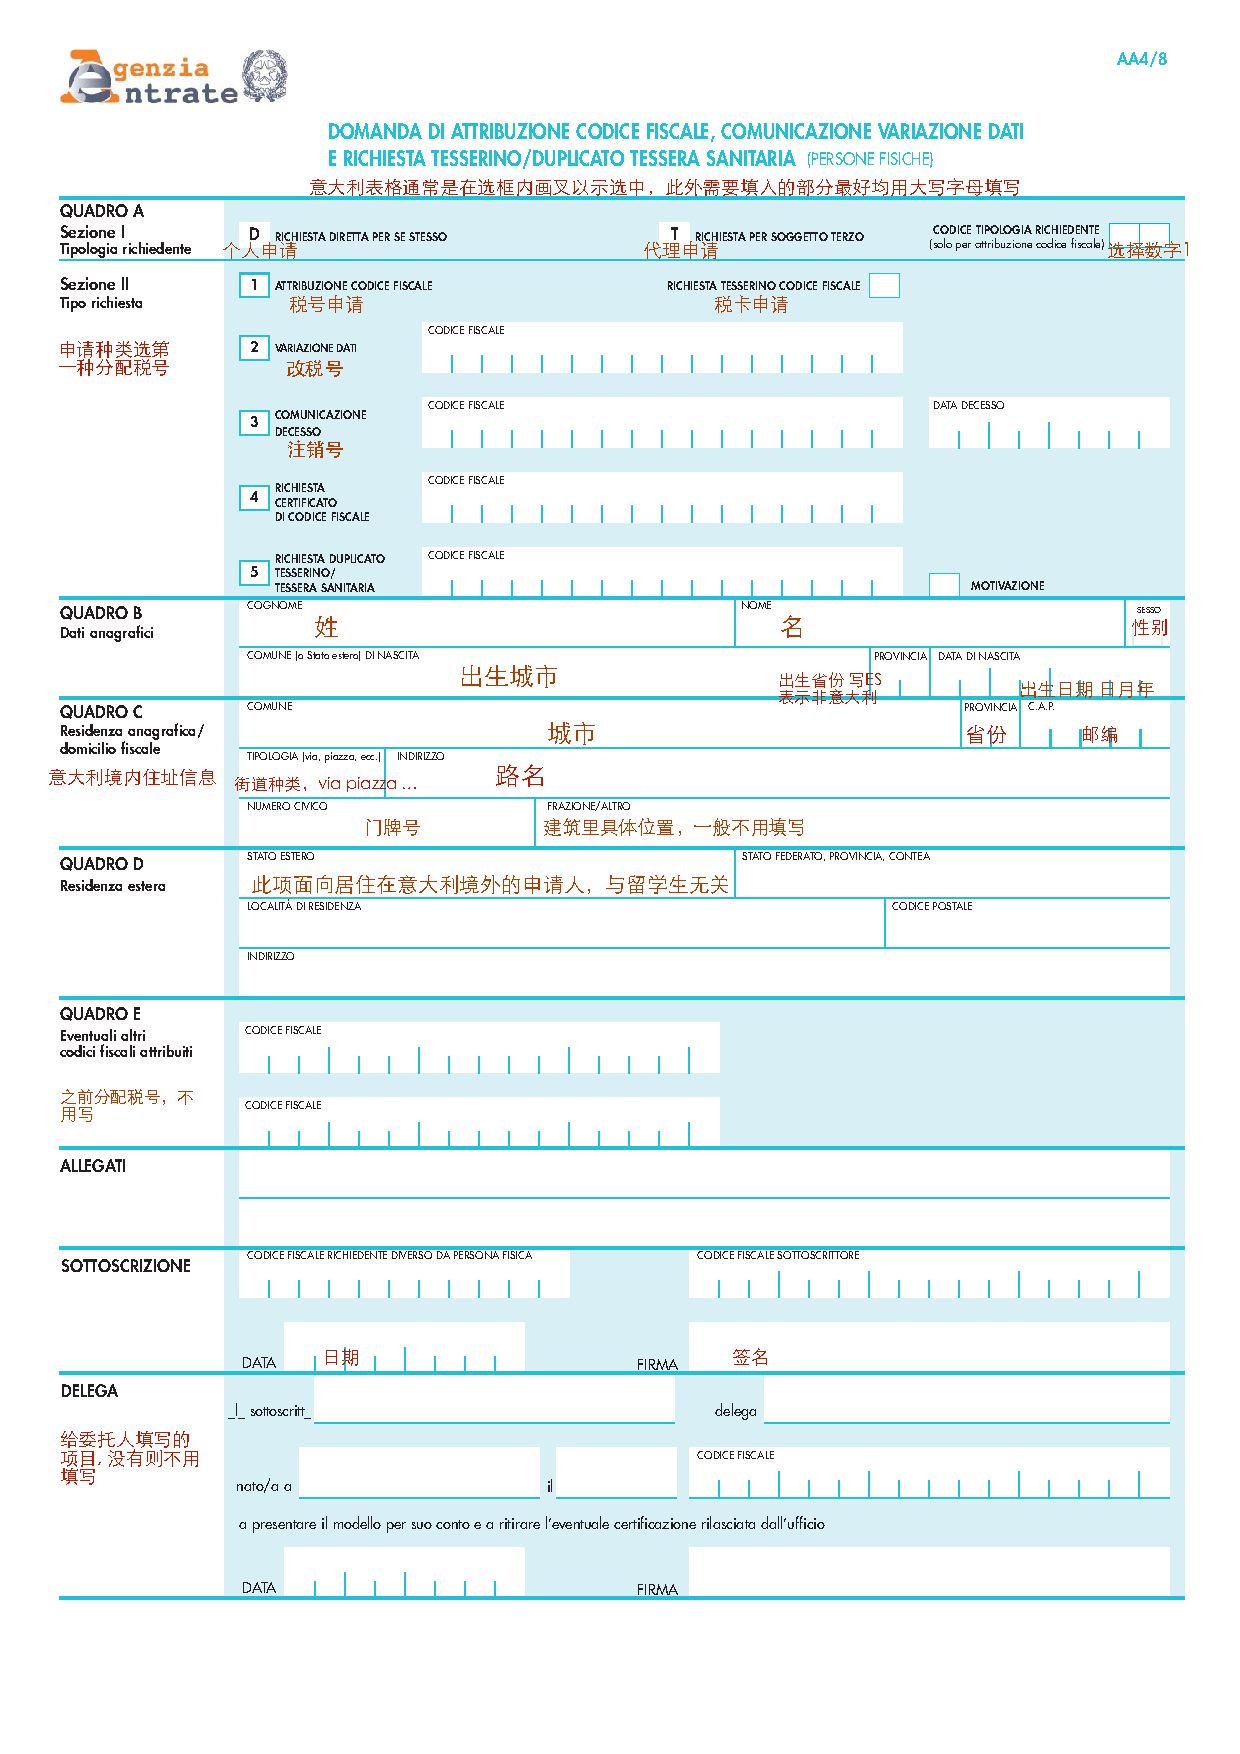
\includepdf{figures/cf.pdf}
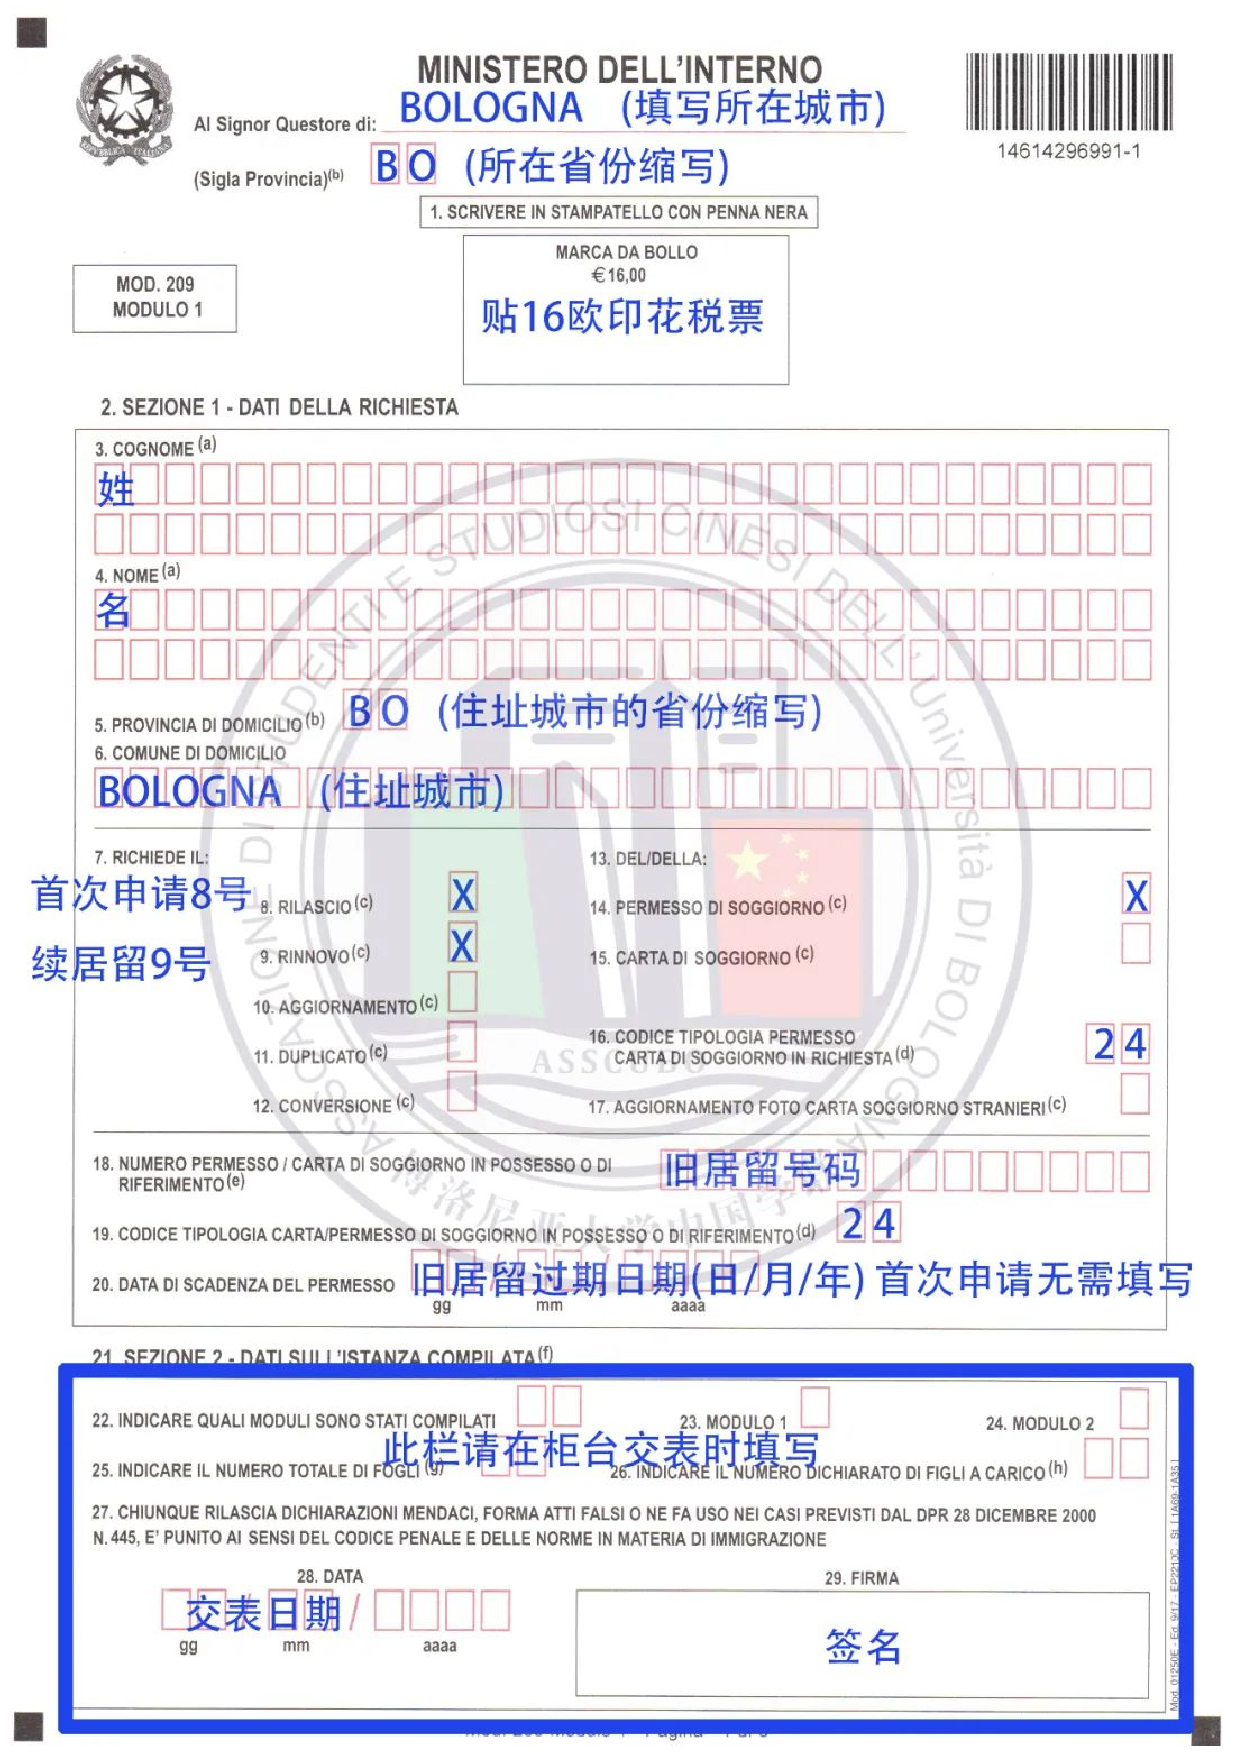
\includepdf{figures/jl1.pdf}
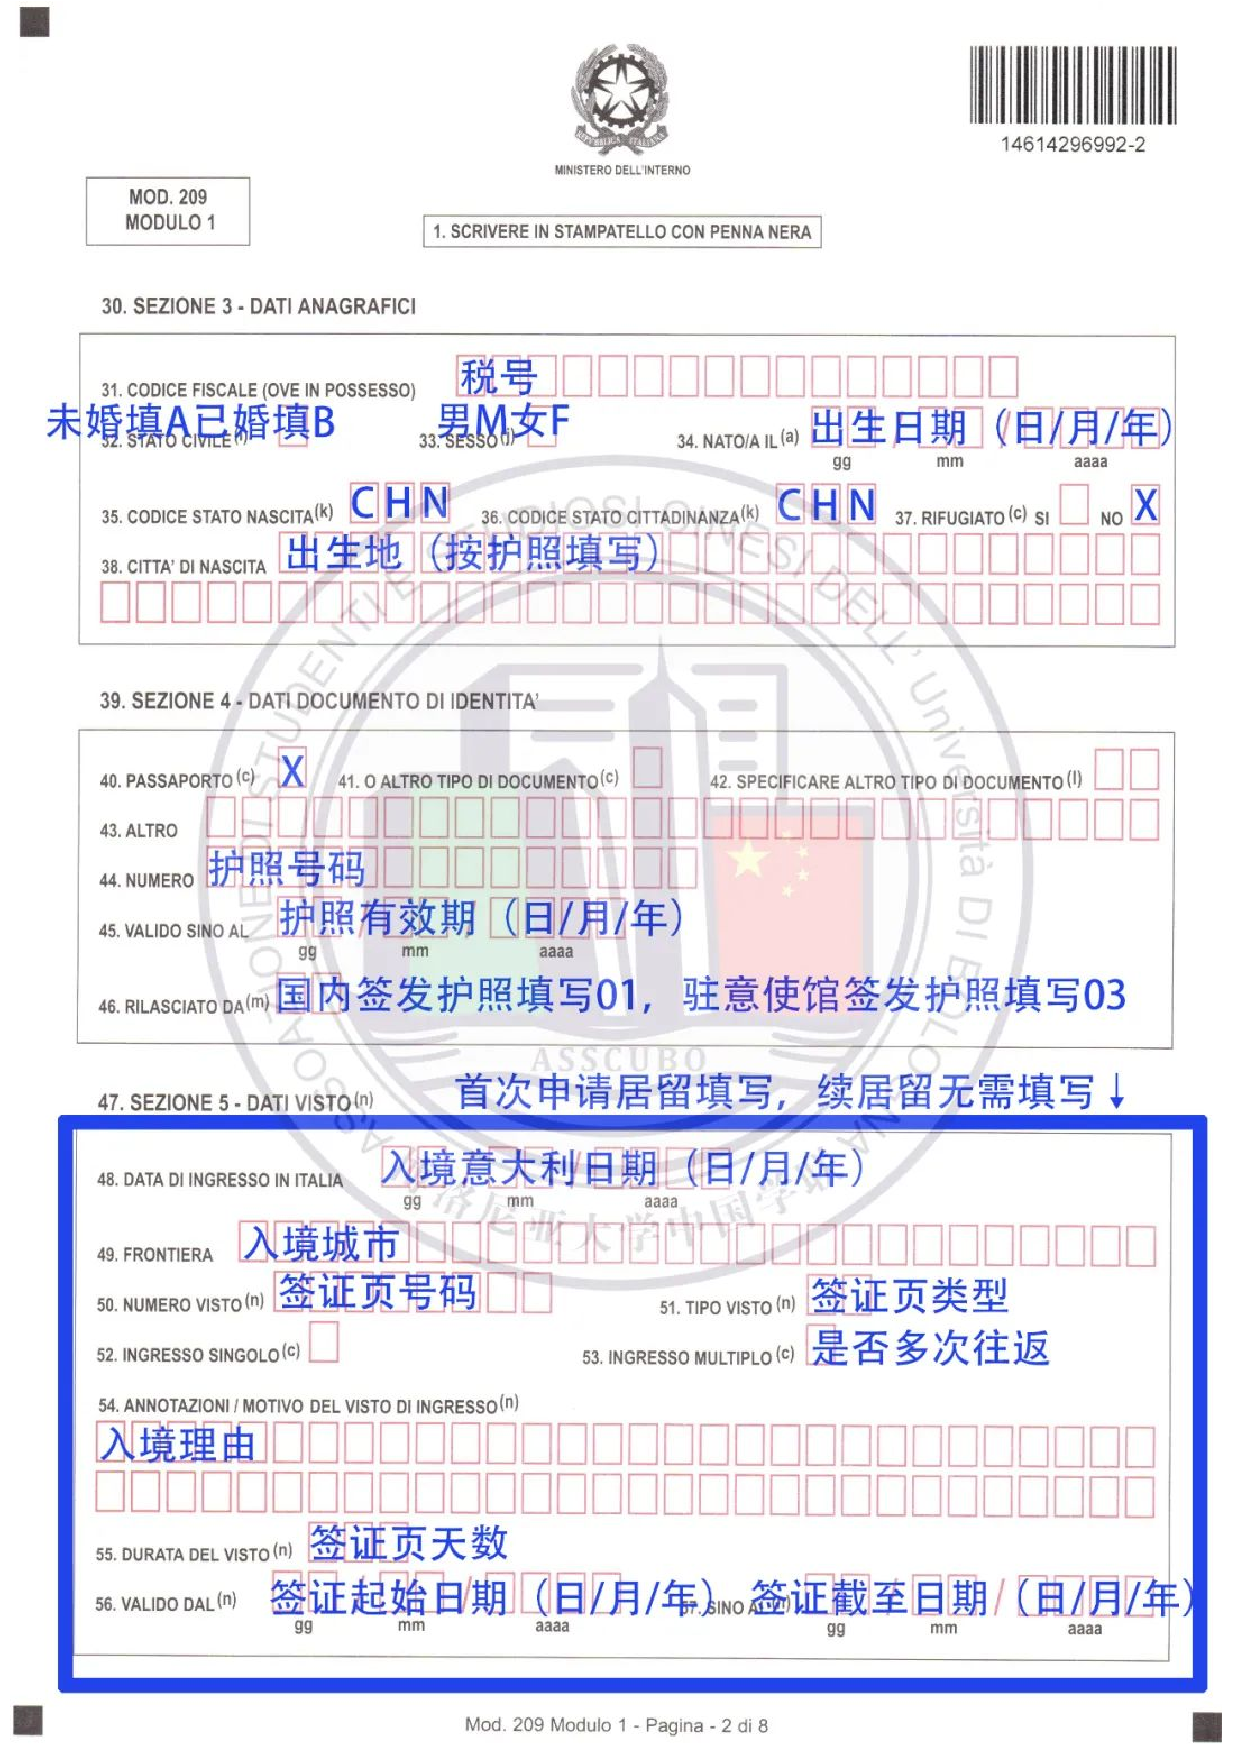
\includepdf{figures/jl2.pdf}
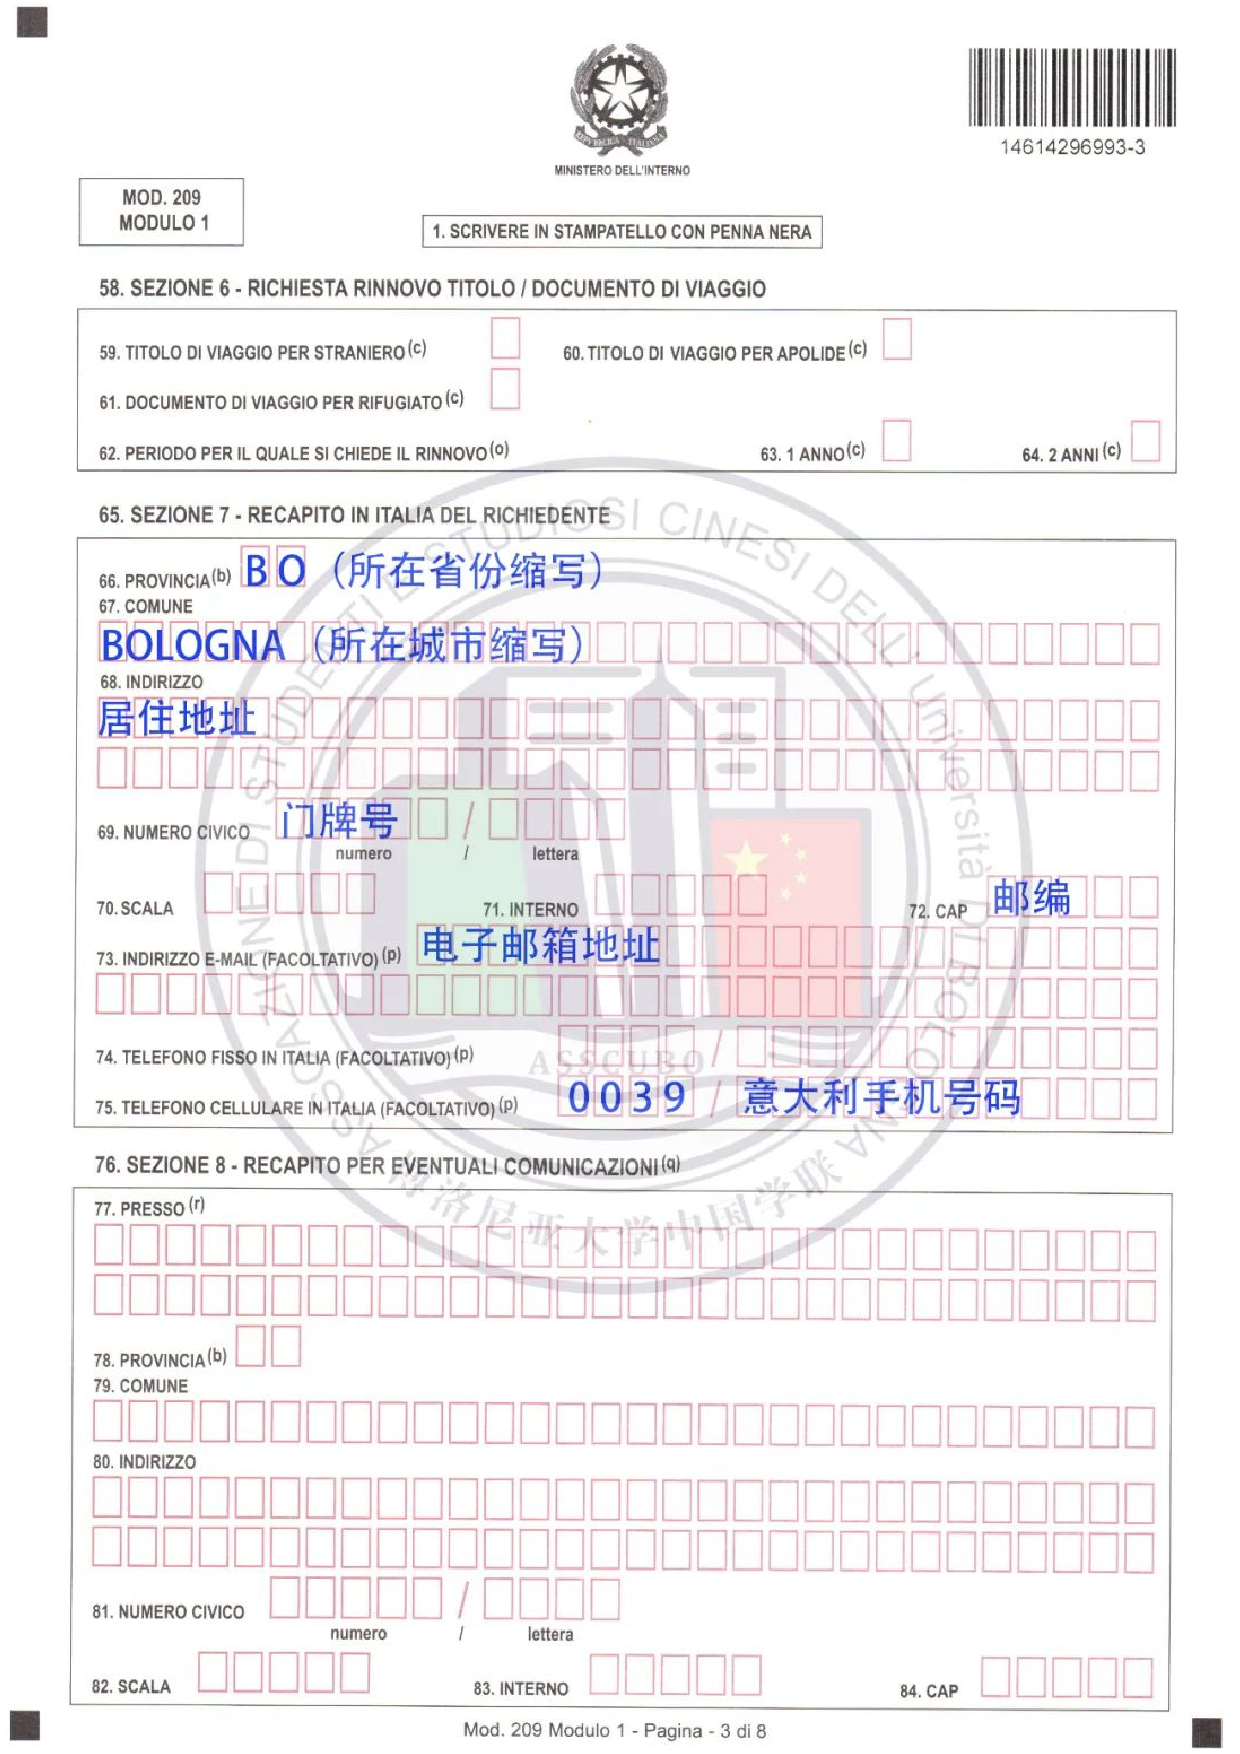
\includepdf{figures/jl3.pdf}
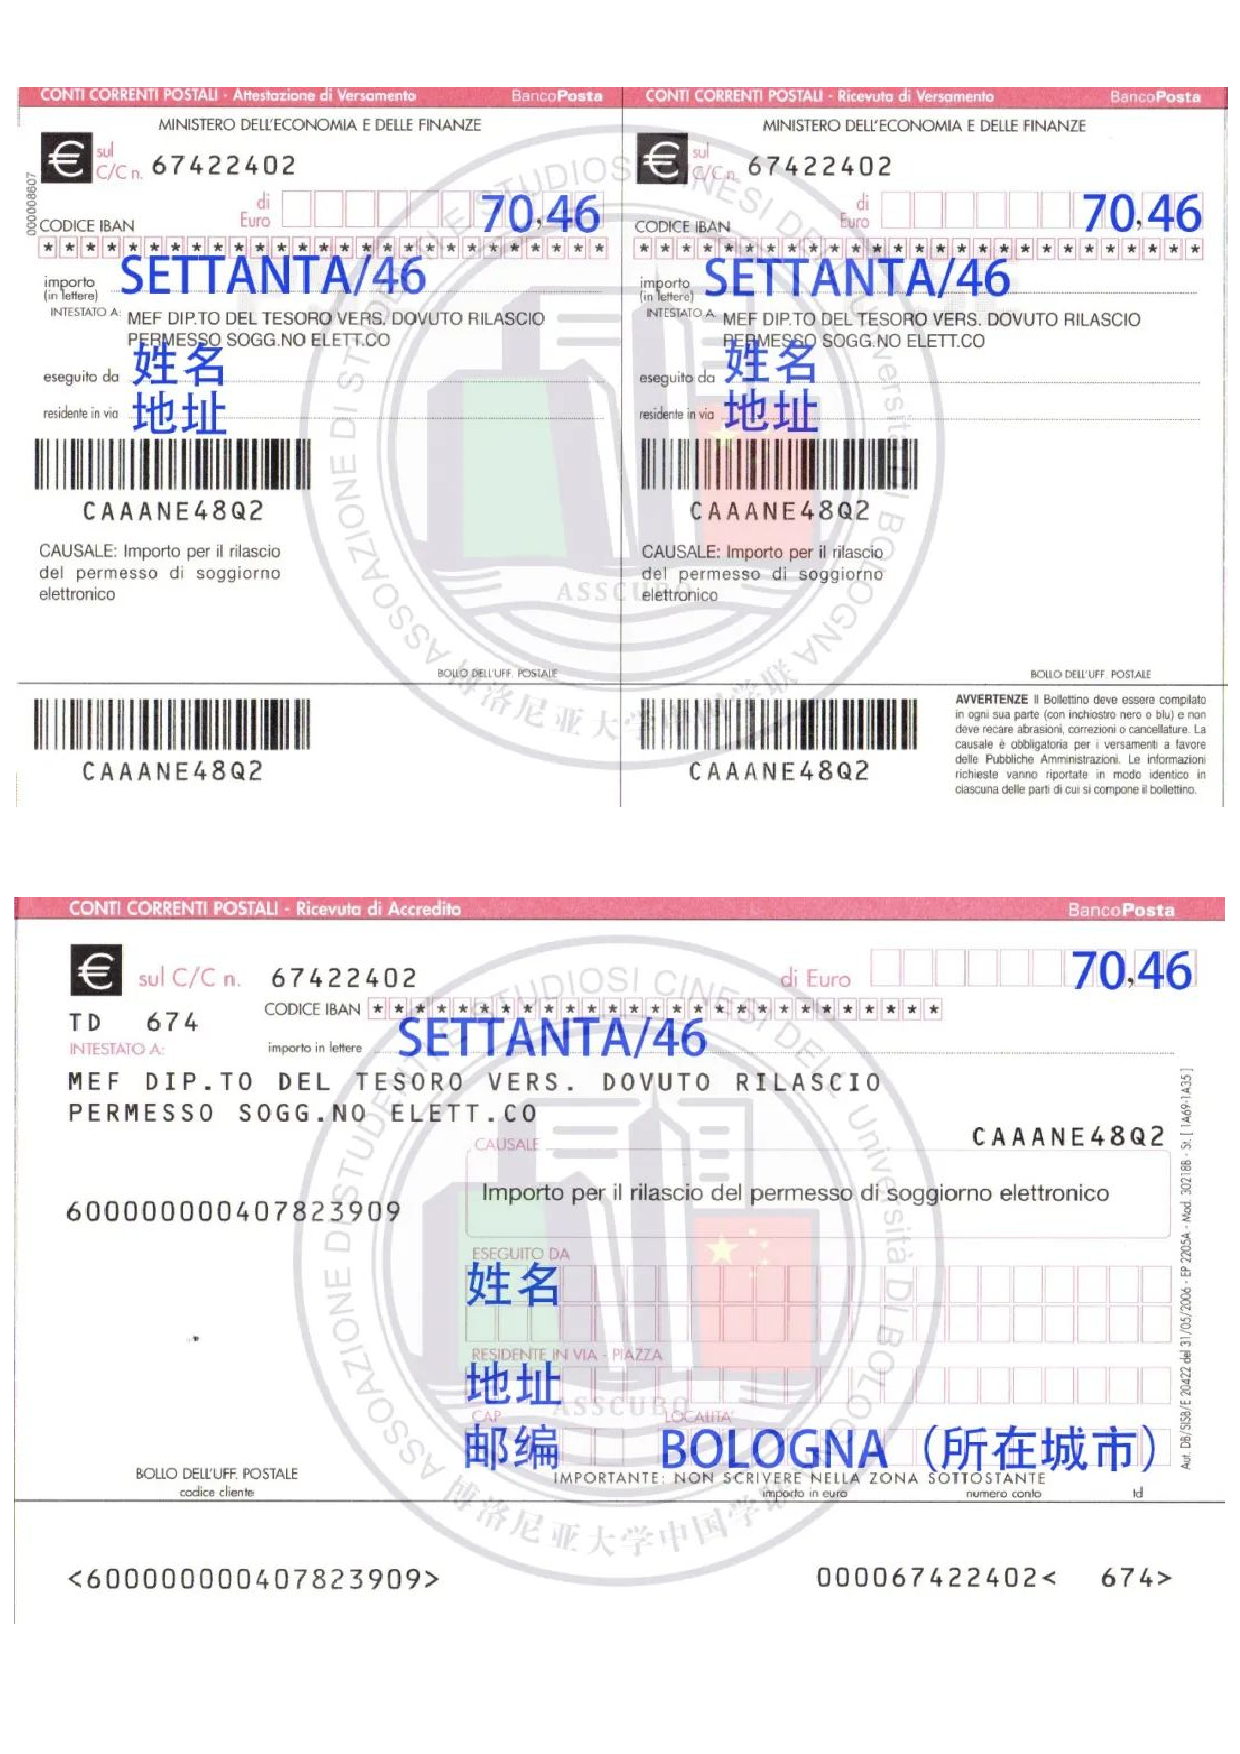
\includepdf{figures/jl4.pdf}
%%%%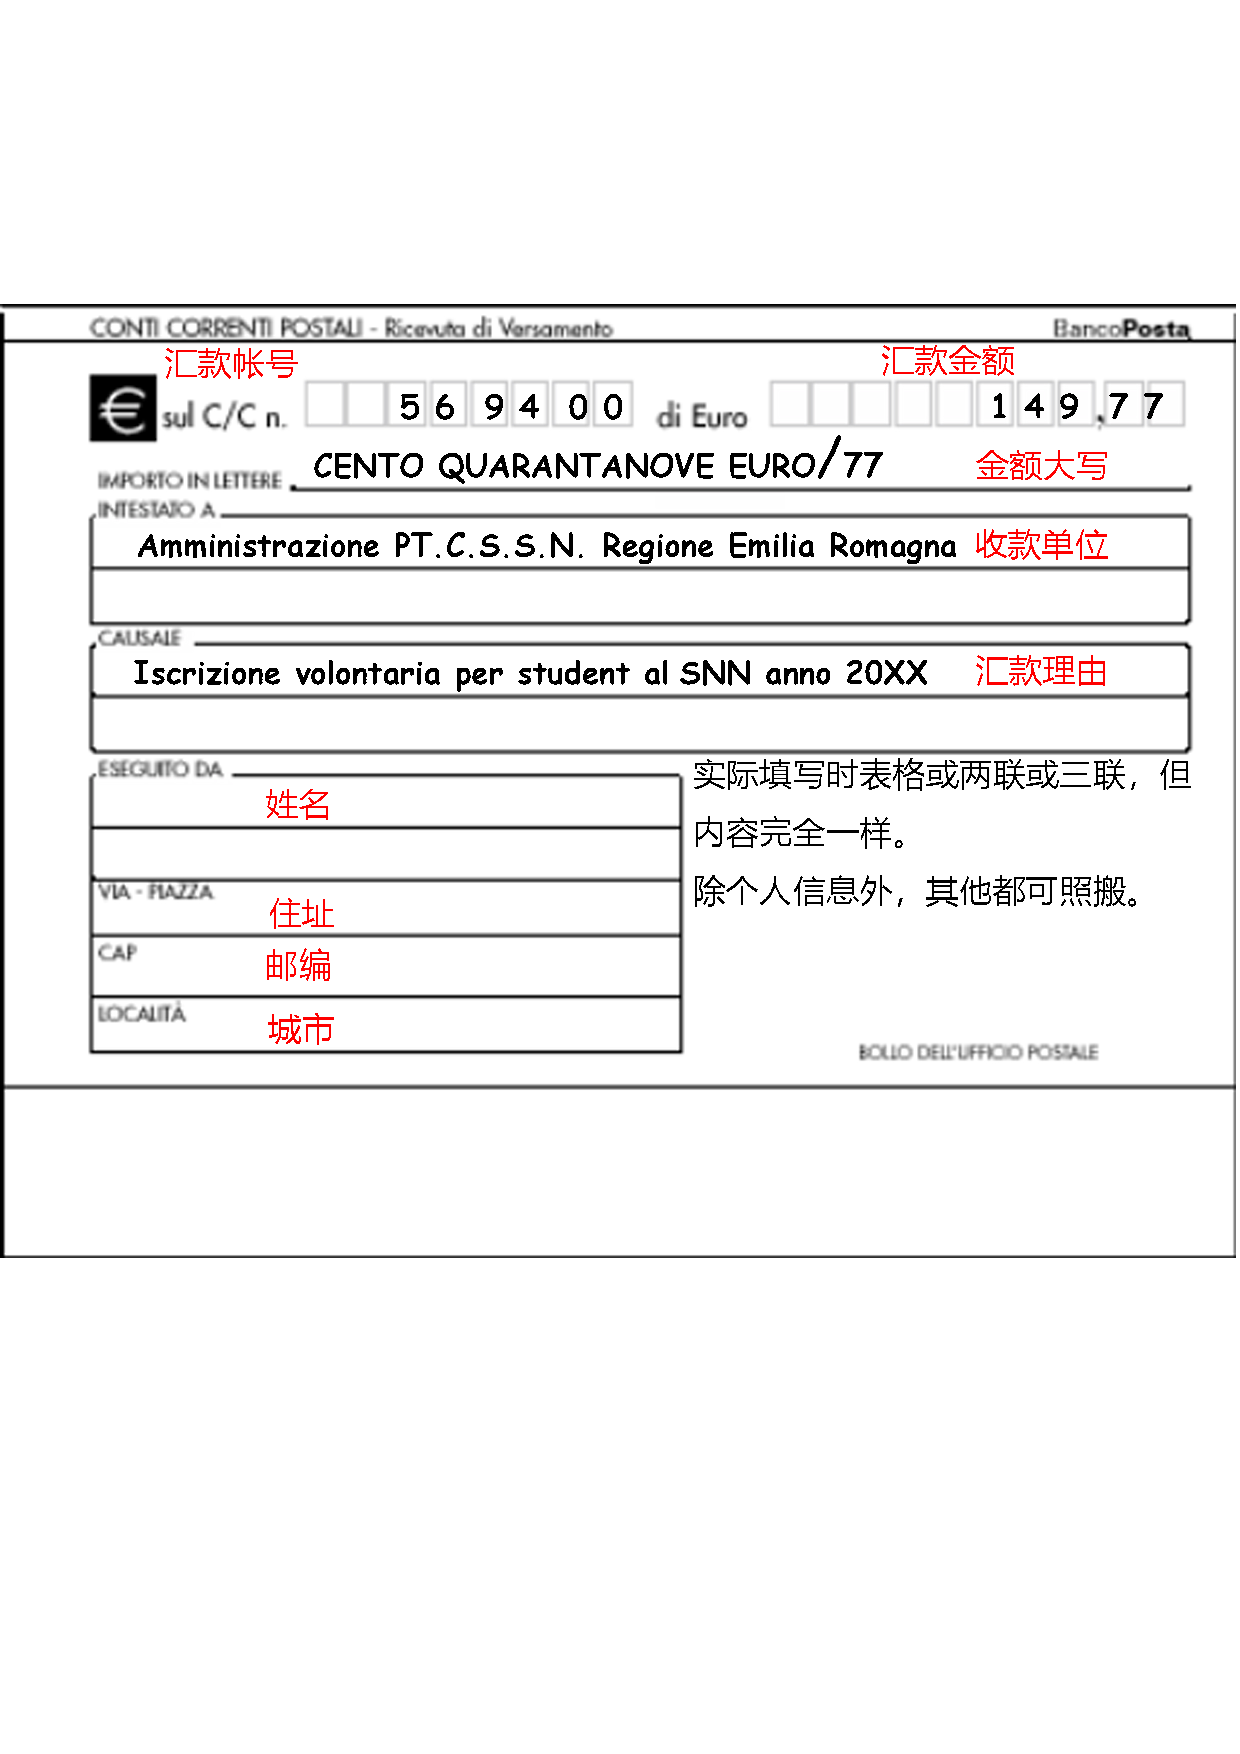
\includepdf{figures/jl5.pdf}2022版注释:保险已不在邮局直接购买,故取消本页面%%%%






\rhead[\fancyplain{}{\bfseries \thechapter \:Appendix}]
{\fancyplain{}{\bfseries\thepage}}


%%%%%%%%%%%%%%%%%%%%%%%%%%%%%%%%%%%%%%%%%%%%%%%%%%%%%%%%%%%%%%%%%%%%%%%%%%%%%%%%%%
% 
%
%  ---     End First Appendix     ---
%
%
%%%%%%%%%%%%%%%%%%%%%%%%%%%%%%%%%%%%%%%%%%%%%%%%%%%%%%%%%%%%%%%%%%%%%%%%%%%%%%%%%%



%%%%%%%%%%%%%%%%%%%%%%%%%%%%%%%%%%%%%%%%%%%%%%%%%%%%%%%%%%%%%%%%%%%%%%%%%%%%%%%%%%
% 
%
%  ---     Second Appendix     ---
%
%
%%%%%%%%%%%%%%%%%%%%%%%%%%%%%%%%%%%%%%%%%%%%%%%%%%%%%%%%%%%%%%%%%%%%%%%%%%%%%%%%%%

\chapter{附录 B, 美院表格}     
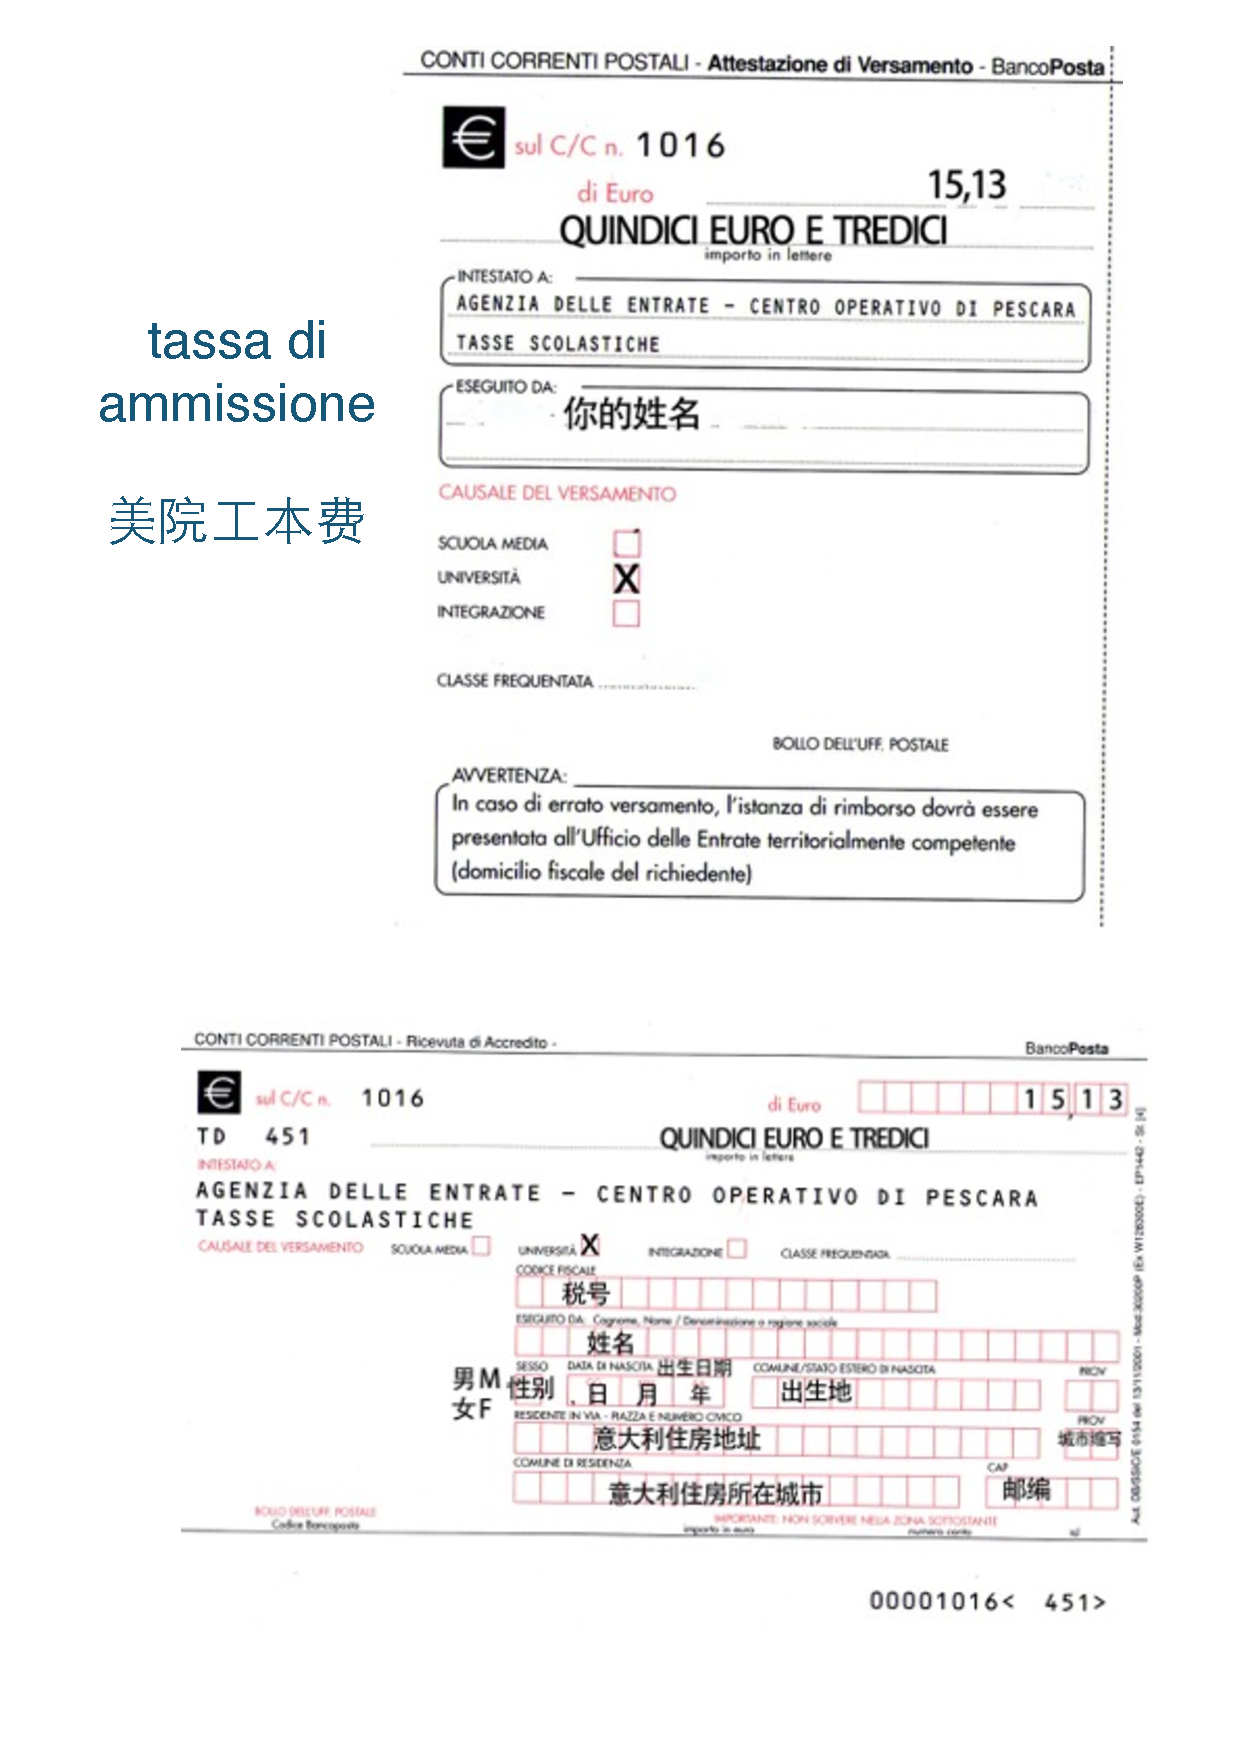
\includepdf{figures/m1.pdf}

\includepdf{figures/zdzm.pdf}

\rhead[\fancyplain{}{\bfseries \thechapter \:Appendix}]
{\fancyplain{}{\bfseries\thepage}} 


%%%%%%%%%%%%%%%%%%%%%%%%%%%%%%%%%%%%%%%%%%%%%%%%%%%%%%%%%%%%%%%%%%%%%%%%%%%%%%%%%%
% 
%
%  ---     thebibliography     ---
%
%
%%%%%%%%%%%%%%%%%%%%%%%%%%%%%%%%%%%%%%%%%%%%%%%%%%%%%%%%%%%%%%%%%%%%%%%%%%%%%%%%%%


\begin{thebibliography}{90}             %crea l'ambiente bibliografia
\rhead[\fancyplain{}{\bfseries \leftmark}]{\fancyplain{}{\bfseries
\thepage}}
%%%%%%%%%%%%%%%%%%%%%%%%%%%%%%%%%%%%%%%%%aggiunge la voce Bibliografia
                                        %   nell'indice
\addcontentsline{toc}{chapter}{参考链接}
\bibitem{irnerio}Irnerio Law https://en.wikipedia.org/wiki/Irnerius
\bibitem{cid}意大利身份证 http://www.comune.bologna.it/cittadino/servizi/9:2931/7422/
\bibitem{unibo}博洛尼亚大学官网 https://www.unibo.it/it
\bibitem{qs}QS世界大学排名 https://www.topuniversities.com/university-rankings/world-university-rankings/2022
\bibitem{times}TIMES世界大学排名 https://www.timeshighereducation.com/world-university-rankings
\bibitem{shanghai}上海交大世界大学排名 https://www.shanghairanking.com/rankings/arwu/2021
\bibitem{usnews}USNews世界大学排名 https://www.usnews.com/education/best-global-universities/rankings
\bibitem{weiji}维基百科 https://zh.wikipedia.org/wiki/Wikipedia:首页
\bibitem{sciopero}意大利罢工查询网址 http://scioperi.mit.gov.it/mit2/public/scioperi/ricerca
\bibitem{tourismbo}博洛尼亚旅游网 http://www.bolognawelcome.com/
\end{thebibliography}
 


%%%%%%%%%%%%%%%%%%%%%%%%%%%%%%%%%%%%%%%%%%%%%%%%%%%%%%%%%%%%%%%%%%%%%%%%%%%%%%%%%%
% 
%
%  ---     Ringraziamenti     ---
%
%
%%%%%%%%%%%%%%%%%%%%%%%%%%%%%%%%%%%%%%%%%%%%%%%%%%%%%%%%%%%%%%%%%%%%%%%%%%%%%%%%%%


%%%%%%%%%%%%%%%%%%%%%%%%%%%%%%%%%%%%%%%%%%%%%%%%%%%%%%%%%%%%%%%%%%%%%%%%%%%%%%%%%%
% 
%
%  ---     Conclusions     ---
%
%
%%%%%%%%%%%%%%%%%%%%%%%%%%%%%%%%%%%%%%%%%%%%%%%%%%%%%%%%%%%%%%%%%%%%%%%%%%%%%%%%%%



% %%%%%%%%%%%%%%%%%%%%%%%%%%%%%%%%%%%%%%%%%non numera l'ultima pagina sinistra
% \clearpage{\pagestyle{empty}\cleardoublepage}
% %%%%%%%%%%%%%%%%%%%%%%%%%%%%%%%%%%%%%%%%%per fare le conclusioni
% \chapter*{鸣谢}


% %%%%%%%%%%%%%%%%%%%%%%%%%%%%%%%%%%%%%%%%%imposta l'intestazione di pagina
% \rhead[\fancyplain{}{\bfseries
% CONCLUSIONS}]{\fancyplain{}{\bfseries\thepage}}
% \lhead[\fancyplain{}{\bfseries\thepage}]{\fancyplain{}{\bfseries
% CONCLUSIONS}}
% %%%%%%%%%%%%%%%%%%%%%%%%%%%%%%%%%%%%%%%%%aggiunge la voce Conclusioni
%                                         %   nell'indice
% \addcontentsline{toc}{chapter}{结束语} 

% 手册制作不容易


\clearpage{\pagestyle{empty}\cleardoublepage}
\chapter*{后言}
\thispagestyle{empty}

本手册由Latex排版,XeLaTeX引擎生成。

\vspace{0.5cm}
项目地址为:https://github.com/youkarin/UnibostudetsC

\vspace{0.5cm}
对于纸质阅读者,文中的部分相关链接均提供了二维码,可以方便您直接扫码访问。对于电子版阅读者,所有链接及二维码均提供点击跳转。

\vspace{0.5cm}
由于人力、技术、美工能力有限,手册难免会有遗漏、错误和遗憾之处,我们希望有善心,又精通相关方面(文案、绘画、制图等)的同学能贡献出自己的力量,让下版手册的质量和颜值超越本版,借此机会证明自己的才华,也可以为自己丰富履历。

\vspace{0.5cm}
如果您想提供反馈、建议、指正,或是想要联系我们,请通过上方链接访问我们的项目并留言。

\vspace{0.5cm}
感谢所有参与本手册编纂的人员,感谢所有提供了帮助的人员,同样感谢正在阅读的您!\\\\

\begin{flushright}
博大学联 \& 博美学联 \\
2022年6月10日
\end{flushright} 
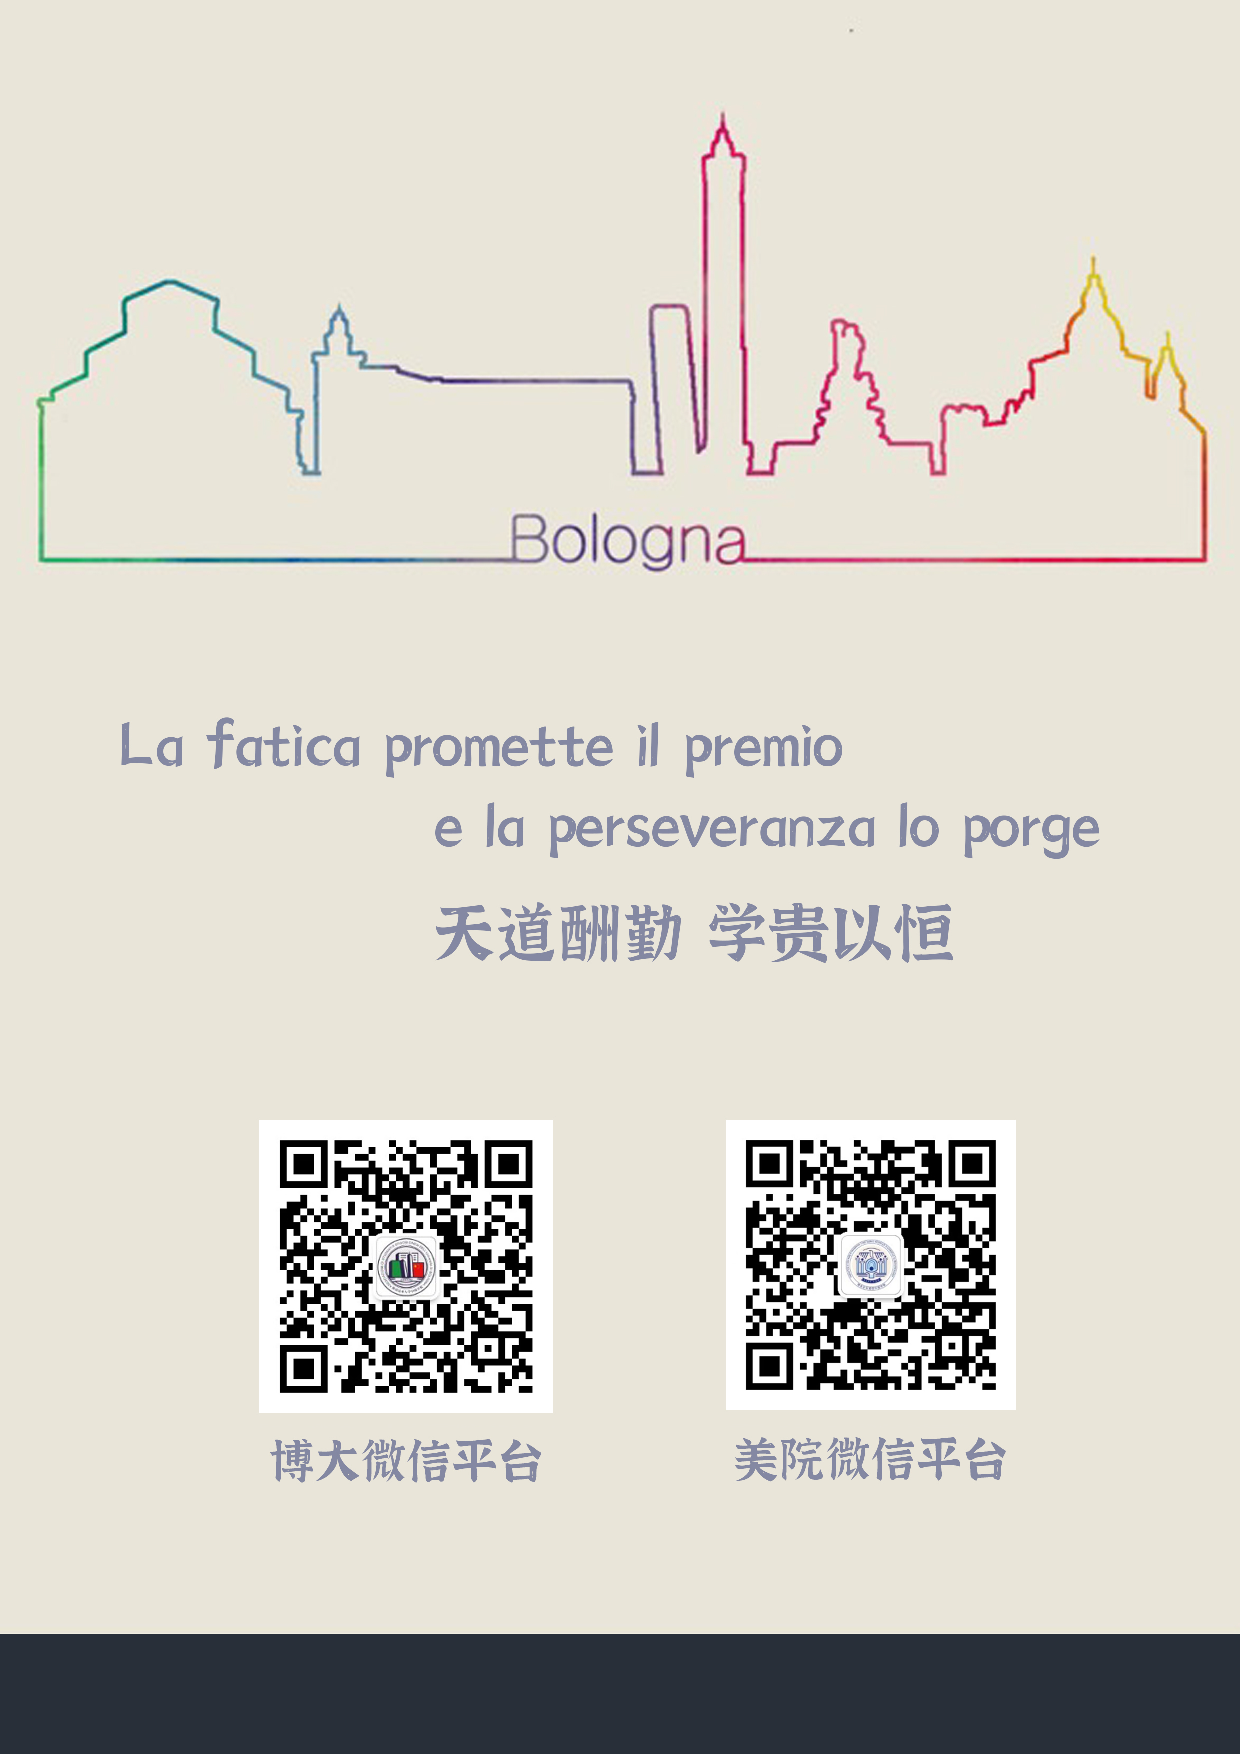
\includepdf{figures/c2.pdf}
%%%%%%%%%%%%%%%%%%%%%%%%%%%%%%%%%%%%%%%%%%%%%%%%%%%%%%%%%%%%%%%%%%%%%%%%%%%%%%%%%%
% 
%
%  ---     End     ---
%
%
%%%%%%%%%%%%%%%%%%%%%%%%%%%%%%%%%%%%%%%%%%%%%%%%%%%%%%%%%%%%%%%%%%%%%%%%%%%%%%%%%%
\end{document}